% ===============================================================
% THESIS ROOT DOCUMENT — DTU layout
% ===============================================================
% Compile with XeLaTeX (Overleaf: Menu > Compiler > XeLaTeX), like Aida's thesis.
\documentclass[10pt,twoside,openright]{book}

% ---------------------------------------------------------------
% Edit these once. Every weekly report and the thesis title page
% pick them up.
% ---------------------------------------------------------------
\newcommand{\projecttitle}{Your thesis title goes here}
\newcommand{\course}{Master Thesis}

% Supervisors, one per line. Used on the weekly title page and the
% thesis cover.
\newcommand{\supervisorlist}{%
  Rasmus R. Paulsen\\
  Kit Mills Bransby \\
  Philip Ruessell Pedersson}

\newcommand{\authorname}{Mathilde Brinch Sørensen}
\newcommand{\studentnumber}{s254124}
\newcommand{\authorline}{\authorname\ (\studentnumber)}

% Date of the current report. Override it in each weekNN.tex with
% \renewcommand{\reportdate}{January 22, 2026}
\newcommand{\reportdate}{\today}

% ---------------------------------------------------------------
% Cover page and information page (page 2). Edit these once.
% ---------------------------------------------------------------
\newcommand{\thesisperiod}{3.\ February 2026 - 3.\ August 2026}
\newcommand{\thesisects}{35 ECTS points}

% Cover image: put the file in figures/ (leave as is to skip it)
\newcommand{\coverimagefile}{coverimage.png}

% "Author" or "Authors" (also used on the cover)
\newcommand{\thesisauthorlabel}{Author}
\newcommand{\thesisauthorsuffix}{}      % set to s for several authors

% --- Cover: one line per person, separated by \\ -----------------
\newcommand{\coverauthors}{\authorname\ (\studentnumber)}
\newcommand{\coversupervisors}{%
  [Title] Rasmus R. Paulsen\\[0pt]
  [Title] Kit Mills Bransby\\[0pt]
  [Title] Philip Ruessell Pedersson}

% --- Page 2 ------------------------------------------------------
% \thesisauthor{Name (student number)}{Programme}{Institution}
\newcommand{\thesisauthor}[3]{#1\par #2\par #3\par\vspace{15.3pt}}
% \thesissupervisor{Title and name}{Affiliation}
\newcommand{\thesissupervisor}[2]{#1\par #2\par\vspace{15.3pt}}

\newcommand{\thesisauthors}{%
  \thesisauthor{\authorname\ (\studentnumber)}{M.Sc. [Your programme]}{Technical University of Denmark}}

\newcommand{\thesissupervisors}{%
  \thesissupervisor{[Title] Rasmus R. Paulsen}{[Department], Technical University of Denmark}
  \thesissupervisor{[Title] Kit Mills Bransby}{[Department / company]}
  \thesissupervisor{[Title] Philip Ruessell Pedersson}{[Department / company]}}

\newcommand{\coverphotonote}{[Describe the cover image and its sources, e.g.\ 3D rendering of \ldots].}
\newcommand{\publisher}{DTU Compute, Department of Applied Mathematics and Computer Science,\newline
Richard Petersens Plads, Building 324, 2800 Kgs.\ Lyngby, Denmark}

% ---------------------------------------------------------------
% Shared preamble. Loaded by main.tex AND by every weekNN.tex.
% Anything you add here is available everywhere, forever.
% ---------------------------------------------------------------

\usepackage{iftex}
\ifPDFTeX
  \usepackage[T1]{fontenc}
  \usepackage[utf8]{inputenc}
  \usepackage{lmodern}
\else
  \usepackage{fontspec}   % Latin Modern is the default body font
\fi
\usepackage[english]{babel}

\usepackage{amsmath,amssymb,mathtools}
\usepackage{graphicx}
\usepackage{subcaption}
\usepackage{booktabs}
\usepackage{tabularx}
\usepackage{longtable}
\usepackage{siunitx}
\usepackage{xcolor}
\usepackage{enumitem}
\usepackage{tcolorbox}
\usepackage[hidelinks]{hyperref}
\usepackage{cleveref}
\usepackage{tikz}
\usetikzlibrary{positioning, arrows.meta, fit, backgrounds, calc, shapes.geometric}
\usepackage{graphicx}   % needed for \resizebox
\usepackage{booktabs}
\usepackage{pdflscape}
\usepackage{adjustbox}
\usepackage{subcaption}
\usepackage{graphicx}
\usepackage{tikz}
\usetikzlibrary{arrows.meta, positioning}
\usepackage{wrapfig}
  \usepackage{tikz}
  \usetikzlibrary{fit, positioning, arrows.meta}
  \usepackage{wrapfig}

\usepackage{placeins}   % add this to your preamble if not already present
% Figures live in one place for the whole project.
\graphicspath{{figures/}}

% Bibliography: one .bib file for weekly reports and thesis alike.
\usepackage[backend=biber,style=numeric,sorting=none,maxbibnames=6]{biblatex}
\addbibresource{refs.bib}

% ---------------------------------------------------------------
% Project notation. Define a symbol ONCE here and never think about
% it again. If you later rename something, you rename it in one line
% and every weekly report plus the thesis follows.
% ---------------------------------------------------------------

% --- Names and abbreviations -----------------------------------
\newcommand{\nnunet}{nnU\nobreakdash-Net}
\newcommand{\dataset}{ImageCAS}          % rename to your dataset
\newcommand{\ourmethod}{ShapeNetX}       % rename to your method

% --- Metrics ----------------------------------------------------
\newcommand{\dsc}{\mathrm{DSC}}
\newcommand{\iou}{\mathrm{IoU}}
\newcommand{\hd}{\mathrm{HD}_{95}}

% --- Math shorthands -------------------------------------------
\newcommand{\R}{\mathbb{R}}
\newcommand{\E}{\mathbb{E}}
\newcommand{\vect}[1]{\mathbf{#1}}
\newcommand{\norm}[1]{\left\lVert #1 \right\rVert}
\DeclareMathOperator*{\argmin}{arg\,min}
\DeclareMathOperator*{\argmax}{arg\,max}

% --- Notes to self (only visible in draft mode) -----------------
% Put \drafttrue in a weekly report, \draftfalse in main.tex, and
% these vanish from the final thesis without you deleting anything.
\newif\ifdraftnotes
\draftnotestrue
\newcommand{\todonote}[1]{\ifdraftnotes\textcolor{orange}{[TODO: #1]}\fi}


% B5 page (176 x 250 mm), margins measured from Aida's thesis
\usepackage[paperwidth=176mm,paperheight=250mm,inner=25.75mm,outer=20.1mm,top=35mm,bottom=31mm,headheight=12pt,headsep=20pt]{geometry}
% ===============================================================
% DTU house style
% Colours and typography follow the DTU design guide
% (https://designguide.dtu.dk). The chapter/heading layout follows
% the DTU Compute thesis convention used in the example theses.
%
% NOTE: the official DTU Thesis Template on Overleaf is XeLaTeX and
% uses Neo Sans, DTU's real heading font, which is licensed and not
% bundled here. This file reproduces the layout in plain pdfLaTeX
% with a Helvetica-metric substitute so it compiles anywhere.
% See setup/README-dtu.md for how to swap in the official one.
% ===============================================================

\usepackage{fancyhdr}
\usepackage{titlesec}
\usepackage{tikz}
\usetikzlibrary{positioning, arrows.meta, fit, backgrounds, calc, shapes.geometric}
\usepackage{graphicx}   % needed for \resizebox
\usepackage{booktabs}
\usepackage{parskip}
\usepackage{setspace}
% --- Official DTU colour palette --------------------------------
% Primary
\definecolor{dtured}{HTML}{990000}      % corporate red
% Secondary
\definecolor{dtublue}{HTML}{2F3EEA}
\definecolor{dtubrightgreen}{HTML}{1FD082}
\definecolor{dtunavy}{HTML}{030F4F}
\definecolor{dtuyellow}{HTML}{F6D04D}
\definecolor{dtuorange}{HTML}{FC7634}
\definecolor{dtupink}{HTML}{F7BBB1}
\definecolor{dtugrey}{HTML}{DADADA}
\definecolor{dtucoral}{HTML}{E83F48}
\definecolor{dtugreen}{HTML}{008835}
\definecolor{dtupurple}{HTML}{79238E}

% Pick the accent colour for the cover and headings. The design
% guide says: one colour, used consistently, throughout.
\colorlet{dtuaccent}{dtured}

% --- Typography -------------------------------------------------
% Headings are set in TeX Gyre Adventor (as in Aida's thesis), body in
% Latin Modern. This needs XeLaTeX or LuaLaTeX (Overleaf: Menu >
% Compiler). Under pdfLaTeX (weekly reports) it falls back to Helvetica.
\usepackage{iftex}
\ifPDFTeX
  \usepackage[scaled=0.92]{helvet}
  \newcommand{\dtuheadfont}{\sffamily}
  \newcommand{\dtuchapfont}{\sffamily}
\else
  \usepackage{fontspec}
  \newfontfamily\dtuheadfont{TeX Gyre Adventor}[Ligatures=TeX]
  \newfontfamily\dtuchapfont{TeX Gyre Adventor}[Ligatures=TeX]
\fi
\colorlet{dtuchapgrey}{black!35}

% --- Headings ---------------------------------------------------
% Chapter: light-grey "CHAPTER" + large red number, right-aligned
% regular-weight title, thin rule underneath.
\makeatletter
\@ifundefined{chapter}{}{%
\titleformat{\chapter}[display]
  {\dtuchapfont\raggedleft}
  {\raggedright{\color{dtuchapgrey}\fontsize{18}{20}\selectfont\MakeUppercase{\chaptertitlename}}\hspace{0.4em}{\color{dtuaccent}\fontsize{40}{44}\selectfont\thechapter}}
  {1.2em}
  {\fontsize{28}{34}\selectfont}
  [\vspace{-28pt}\rule{\linewidth}{0.6pt}]
\titleformat{name=\chapter,numberless}[display]
  {\dtuchapfont\raggedleft}{}{0pt}{\fontsize{28}{34}\selectfont}
  [\vspace{-28pt}\rule{\linewidth}{0.6pt}]
\titlespacing*{\chapter}{0pt}{-40.7pt}{4pt}
\titlespacing*{name=\chapter,numberless}{0pt}{-40.7pt}{4pt}
}
\makeatother

\titleformat{\section}{\dtuheadfont\fontsize{14}{17}\selectfont}{\thesection}{0.8em}{}
\titleformat{\subsection}{\dtuheadfont\fontsize{12}{15}\selectfont}{\thesubsection}{0.8em}{}
\titleformat{\subsubsection}{\dtuheadfont\fontsize{10}{13}\selectfont}{\thesubsubsection}{0.8em}{}
\titlespacing*{\section}{0pt}{2.2ex plus 1ex minus .2ex}{1.2ex plus .2ex}
\titlespacing*{\subsection}{0pt}{2ex plus 1ex minus .2ex}{1ex plus .2ex}

% Captions: bold label, small text
\usepackage[font=small,labelfont=bf,labelsep=quad]{caption}
% Paragraphs indented, no vertical space (as in Aida's thesis)
\setlength{\parindent}{0pt}
\setlength{\parskip}{4pt}
\setstretch{1.1}  

% --- Running heads ----------------------------------------------
% Even: page number left, chapter right. Odd: section left, page right.
\pagestyle{fancy}
\fancyhf{}
\renewcommand{\headrulewidth}{0.4pt}
\makeatletter
\@ifundefined{chapter}{}{\renewcommand{\chaptermark}[1]{\markboth{\thechapter\ #1}{}}}
\makeatother
\renewcommand{\sectionmark}[1]{\markright{\thesection\ #1}{}}
\fancyhead[LE,RO]{\dtuheadfont\footnotesize\thepage}
\fancyhead[RE]{\dtuheadfont\footnotesize\nouppercase{\leftmark}}
\fancyhead[LO]{\dtuheadfont\footnotesize\nouppercase{\rightmark}}
\fancypagestyle{plain}{\fancyhf{}\renewcommand{\headrulewidth}{0pt}}

% Blank pages inserted by openright: no header
\makeatletter
\def\cleardoublepage{\clearpage\if@twoside\ifodd\c@page\else
  \hbox{}\thispagestyle{empty}\newpage\fi\fi}
\makeatother

% --- Logo -------------------------------------------------------
% ---------------------------------------------------------------
% DTU logo.
% If figures/dtu_logo.pdf exists it is used. Otherwise a TikZ
% approximation of the wordmark plus the three wave elements is
% drawn so the project always compiles. Replace it with the real
% file from the design guide before you submit anything.
% ---------------------------------------------------------------
\newcommand{\dtulogo}[1][3.2cm]{%
  \IfFileExists{figures/dtu_logo.pdf}
    {\includegraphics[width=#1]{dtu_logo.pdf}}
    {\begin{tikzpicture}[x=#1/4,y=#1/4]
       \node[text=dtuaccent,anchor=south,
             font=\sffamily\bfseries\fontsize{34}{34}\selectfont,
             inner sep=0pt,scale=#1/3.2cm] at (2,0.55) {DTU};
       \foreach \y in {0,-0.62,-1.24}{%
         \fill[dtuaccent]
           (0,\y) -- (1,\y+0.26) -- (2,\y) -- (3,\y+0.26) -- (4,\y)
                 -- (3,\y-0.26) -- (2,\y) -- (1,\y-0.26) -- cycle;}
     \end{tikzpicture}}}


% --- Cover page -------------------------------------------------
% Layout follows the DTU Compute thesis cover: red marker + "DTU Compute",
% bold title, optional cover image, authors, supervisors, DTU logo.
% \dtucover{place and year}   e.g. \dtucover{Kongens Lyngby 2026}
% Put your cover image in figures/ and set \coverimagefile in project.tex.
\newcommand{\dtucover}[1]{%
  \begin{titlepage}
  \thispagestyle{empty}
  \begin{tikzpicture}[remember picture,overlay,x=1pt,y=1pt]
    % Red marker and department name
    \fill[dtuaccent] ([shift={(50.5,-103)}]current page.north west) rectangle
      ++(3,-18);
    \node[anchor=north west,inner sep=0pt,align=left,font=\dtuheadfont\fontsize{9}{11}\selectfont]
      at ([shift={(58,-102)}]current page.north west)
      {DTU Compute\\[1pt]{\color{black!55}Department of Applied Mathematics and Computer Science}};
    % Title and thesis type
    \node[anchor=north west,inner sep=0pt,text width=400pt,align=left]
      at ([shift={(50.5,-137)}]current page.north west)
      {{\dtuheadfont\bfseries\fontsize{20}{22}\selectfont\projecttitle\par}
       \vspace{6pt}
       {\dtuheadfont\fontsize{13}{16}\selectfont\course\par}};
    % Cover image (optional)
    \IfFileExists{figures/\coverimagefile}{%
      \node[anchor=north,inner sep=0pt]
        at ([shift={(0,-235)}]current page.north)
        {\includegraphics[width=255pt]{\coverimagefile}};}{}
    % Authors and supervisors
    \node[anchor=north west,inner sep=0pt,text width=330pt,align=left,
          font=\dtuheadfont\fontsize{10}{17.9}\selectfont]
      at ([shift={(50.5,-428)}]current page.north west)
      {{\bfseries Author\thesisauthorsuffix:}\\[0pt] \coverauthors\\[17.9pt]
       {\bfseries Supervisors:}\\[0pt] \coversupervisors};
    % Logo and place/year
    \node[anchor=south east,inner sep=0pt]
      at ([shift={(-44,68)}]current page.south east) {\dtulogo[1.2cm]};
    \node[anchor=north west,inner sep=0pt,font=\dtuheadfont\fontsize{8}{10}\selectfont]
      at ([shift={(50.5,-612)}]current page.north west) {#1};
  \end{tikzpicture}
  \null
  \end{titlepage}}

% --- Information page (second page) -----------------------------
% Title, period, ECTS, authors, supervisors with affiliations, cover
% photo note and publisher. All text is set in project.tex.
\newcommand{\dtuinfopage}{%
  \thispagestyle{empty}
  \begingroup
  \dtuheadfont\fontsize{8.5}{15.3}\selectfont
  \setlength{\parindent}{0pt}
  \vspace*{45pt}
  {\bfseries\projecttitle}\par
  \course\par
  \thesisperiod\par
  \thesisects\par
  \vspace{15.3pt}
  {\bfseries\thesisauthorlabel}\par
  \thesisauthors
  {\bfseries Supervisors}\par
  \thesissupervisors
  \vspace{4pt}
  \begin{tabular}{@{}p{2.2cm}>{\raggedright\arraybackslash}p{\dimexpr\linewidth-2.2cm\relax}@{}}
    \bfseries Cover photo: & \coverphotonote\\[6pt]
    \bfseries Published by: & \publisher
  \end{tabular}
  \endgroup
  \clearpage}

% --- Weekly-report banner ---------------------------------------
% A slim version of the cover for the short reports.
\newcommand{\dtuweeklyhead}[2]{%
  \noindent\begin{minipage}[b]{0.72\linewidth}
    {\dtuheadfont\bfseries\LARGE \projecttitle\par}\vspace{0.3em}
    {\dtuheadfont\large\color{dtuaccent} Weekly Report #1 \normalcolor\quad\small #2\par}
  \end{minipage}\hfill
  \begin{minipage}[b]{0.24\linewidth}\raggedleft\dtulogo[1.8cm]\end{minipage}
  \vspace{0.5em}
  {\color{dtuaccent}\hrule height 1.2pt}
  \vspace{0.9em}
  \noindent\begin{tabular}{@{}r@{\hspace{1em}}l@{}}
    \dtuheadfont\bfseries Course      & \course \\
    \dtuheadfont\bfseries Supervisors &
      \begin{tabular}[t]{@{}l@{}}\supervisorlist\end{tabular} \\
    \dtuheadfont\bfseries Author      & \authorline \\
  \end{tabular}
  \vspace{1.4em}}


% Turn off draft-only notes in the final document.
\draftnotesfalse

% While drafting, uncomment to compile only one chapter.
% \includeonly{content/methods}

\begin{document}

\dtucover{Kongens Lyngby 2026}
\dtuinfopage

\frontmatter
\pagestyle{fancy}
\chapter*{Abstract}
\addcontentsline{toc}{chapter}{Abstract}

% One page. The problem, what you did, what you found. Write it last.
Write the abstract here.

\chapter*{Preface}
\addcontentsline{toc}{chapter}{Preface}

This thesis [short description of what the thesis is about].

The thesis was prepared in collaboration with [section / department / company].

The project lasted from [start date] to [end date] and was carried out in
fulfilment of the requirements for the Master of Science degree in
[your programme] at the Technical University of Denmark (DTU).

The reader is assumed to have a fundamental knowledge of [prerequisites].

% Signature: put a scanned signature at figures/signature.png (optional).
% For two authors, copy the \sigblock line into a second column.
\newcommand{\sigblock}[2]{%
  \begin{minipage}[t]{0.45\linewidth}\centering
    \IfFileExists{figures/#1}{\includegraphics[height=1.6cm]{#1}}{\rule{0pt}{1.6cm}}\\[2pt]
    #2
  \end{minipage}}
\vspace{3.5cm}
\begin{center}
  \sigblock{signature.png}{\authorname\ (\studentnumber)}\\[1.2em]
  Kongens Lyngby, \today
\end{center}

\chapter*{Acknowledgements}
\addcontentsline{toc}{chapter}{Acknowledgements}

First, I would like to thank my supervisors for their guidance and support
throughout the project.

Thank the people and institutions that contributed data, advice or
infrastructure, and friends and family for their support.

\section*{AI-Assisted Work Disclosure}
Describe here which AI tools were used and for what, in accordance with DTU's
guidelines. All AI-generated content was reviewed and verified by the author.

\chapter*{Abbreviations}
\addcontentsline{toc}{chapter}{Abbreviations}

% One row per abbreviation, alphabetical: \abbrev{short}{long}
% Same text size, width and spacing as Abstract, Preface and Acknowledgements.
\newcommand{\abbrev}[2]{\textbf{#1} & #2 \\}
\renewcommand{\arraystretch}{1.1}
\noindent
\begin{longtable}{@{}p{2.6cm}@{}p{\dimexpr\linewidth-2.6cm\relax}@{}}
\abbrev{AI}{Artificial Intelligence}
\abbrev{CAD}{Coronary Artery Disease}
\abbrev{CCTA}{Coronary Computed Tomography Angiography}
\abbrev{CT}{Computed Tomography}
\abbrev{DSC}{Dice Similarity Coefficient}
\end{longtable}


\tableofcontents
\mainmatter

% Introduction -- written from scratch on 2026-10-02 after the 2026-09-07 rejection.
% Rewritten 2026-10-04 after the funnel of thesis/style_guide_aida.md (her ch. 1): one step per
% paragraph, claims only. Paragraph 1 is fixed. Evidence cut from here and still owed to the
% State of the Art: 196 patients, left main bifurcation angle 35.5 to 178 degrees
% \cite{temov2016bifurcation}; 136 autopsy hearts, no visible narrowing until plaque fills about 40\%
% of the cross-section \cite{glagov1987remodeling}. The 127-patient curvature result is already in
% clinical_background/05_hemodynamics.tex.
% 2026-10-04: limitations paragraph trimmed to a problem statement; the evidence (Han, Tello Ayala,
% Glagov, Temov) now lives in literature_review.tex. "considers only" softened to "rests on", since
% chan2024orfan shows imaging already refines risk in referred patients. shen2026geometry replaced
% by kashyap2022tortuosity and zebicmihic2024index (Shen excluded thesis-wide, user 2026-10-04).
% 2026-10-05: paragraph 4 reordered to match the review (measurement = Sec. 2, timing = Sec. 3);
% zebicmihic2024index swapped for cui2017bifurcation so every cited study is discussed in the review.
% No forward references in this chapter (user).

\chapter{Introduction}
\label{ch:introduction}
Cardiovascular disease is the leading cause of death worldwide, accounting for an estimated 19.2
million deaths in 2023 \cite{stark2025gbd}.
Coronary artery disease (CAD) is the largest single contributor, responsible for nearly half of
these deaths \cite{stark2025gbd}.
It develops when plaque builds up in the walls of the coronary arteries, which supply the heart
muscle with blood.
The plaque slowly narrows the arteries and can, in extreme cases, rupture, forming a clot that
blocks blood flow and causes a heart attack \cite{libby2019atherosclerosis}.

Plaque does not form evenly along the coronary tree, even though risk factors such as high blood
pressure, high cholesterol and smoking reach every segment through the blood.
Instead, it tends to collect where the drag of the blood flow on the vessel wall is low or
oscillating \cite{chatzizisis2007ess}.
This drag is known as wall shear stress, and it is low mainly on the outer wall just after a
bifurcation and on the inner wall of a bend \cite{asakura1990flow}.
Where plaque forms is therefore tied to the geometry of the tree, which, unlike shear, can be
measured directly from an image.

Coronary geometry varies considerably between individuals \cite{temov2016bifurcation}, so some
trees contain more extensive low-shear regions than others.
Predisposition to plaque may therefore depend not only on systemic risk factors but also on the
anatomy of the individual's own arteries.
Standard risk assessment, however, rests on the former, combining age, sex, smoking, blood
pressure and cholesterol into a single score \cite{score2_2021}.

Whether geometry adds to such a score remains unknown.
Studies relating geometry to plaque have defined geometry inconsistently, and the definition can
decide whether a relationship is found \cite{cui2017bifurcation,kashyap2022tortuosity}.
Most also measured geometry in referred patients whose plaque was already present, so the geometry
may be a consequence of the disease rather than its cause \cite{han2022plaque}.

The aim of this thesis is to test whether coronary geometry, measured before any symptoms of heart
disease, can categorize individuals by their risk of developing plaque.
Rather than referred patients, this work uses adults selected at random from the population of
greater Copenhagen by the Copenhagen General Population Study (CGPS) and scanned for research with
coronary computed tomography angiography (CCTA) \cite{fuchs2023cgps}.
A longitudinal subset of these individuals was scanned a second time 10 years later.
The work proceeds in two stages.
First, an automatic pipeline is developed that segments the coronary tree, assigns each vessel to
its coronary artery and computes branching angles, branch radius ratios and vessel curvature.
Second, these features are used to predict which individuals develop new plaque at a second scan.
Two risk models are compared: a logistic regression on summary features and a transformer that reads
the full curvature profile along each artery.
% TODO (author): baseline open until the CGPS variables are checked. If every SCORE2 marker is
% available the baseline is all of them; otherwise name the subset used.
Both are judged by how much they improve on a baseline model of conventional risk factors, and both are fitted
separately for each coronary artery, since shear acts locally.

Together, these stages establish an automated workflow that measures coronary geometry at population
scale and tests its link to plaque.
If geometry does carry risk, the workflow can identify individuals at increased risk from CCTA scans
that are already acquired.
If it does not, the result indicates that the localization of plaque within a tree does not translate
into a difference in risk between individuals, and the workflow remains a tool for research on
coronary anatomy and CAD.

% Literature Review -- chapter opening. Section files are included in numeric order from
% content/litterature_review.tex (split into one file per section 2026-11-07).
% Literature Review. Rewritten 2026-10-04 from reports/Literature review quality assessment.md and
% revised the same day from reports/Literature review quality assessment 2.md (plan:
% ~/.claude/plans/virtual-herding-flute.md). Modelled on Jimenez Ordonez (2026) Sec. 1.1, see
% thesis/style_guide_sota_aida.md. Re-voiced 2026-10-04 (user): the phrasing and paragraph wrap-ups
% of the first version ("Using ... relies on", "Computational studies have also explored",
% "Machine learning has also been used", "Despite these advancements", "Bridging this gap is
% essential", "The integration of ...") with every correction and added study of the revision kept.
% Table: four studies relating a measured geometry to disease in patients (as Aida's four-row table
% covers one strand); columns make the gap visible (cohort, approach, timing).
% Condensed 2026-10-04 to fit 3 pages (user): material already in the introduction dropped (Asakura
% detail, Temov variation, SCORE2 description); Bekircavusoglu, Zebic Mihic, Givehchi and the
% Chatzizisis mechanism no longer cited here (Zebic Mihic and Temov remain in the introduction).
% Order: S1 history + Asakura (Korona pattern), van der Giessen, Stone 2012 | Kashyap, Zhang, Garcha (chronological) |
% Griffo | S2 Cui (choice of angle; Givehchi dropped 2026-10-04, measurement error is not the point) | tortuosity (Groves, Li, Zebic Mihic 2024, Nannini, Tello Ayala;
% reconciled by endpoint) | extraction (Bransby, Nannini), per-artery scope | S3 Temov variation,
% Juan, Bekircavusoglu, Tommasino | Tello Ayala transformer + Glagov | Han | Sakellarios, Won |
% SCORE2, Chan, Bergstrom | gap | search statement | table.
% shen2026geometry deliberately NOT cited anywhere in the thesis (user, 2026-10-04).
% Rules: author and year as subject, \cite after the year; no numbers in the prose (cohort sizes in
% the table only); no concept explanations; no inserted clauses between two commas; no em dashes;
% synthesis only when every element is cited.
% Full text read: kashyap, li, griffo, telloayala, zhang2024curvature, won2022paradigm, chan2024orfan,
% bergstrom2021scapis, han2022plaque, tommasino2024clap, cui2017bifurcation, zebicmihic2024index,
% nannini2024characterization, juan2017bifurcation, garcha2025sensitivity; vandergiessen and
% sakellarios via the publisher page (quotes to confirm by eye).
% Mechanism (Chatzizisis, Murray, measure definitions) lives in clinical_background/05_hemodynamics.tex.
% Abstract-level only: asakura1990flow, stone2012prediction, groves2009tortuosity,
% bekircavusoglu2026ramus, temov2016bifurcation, glagov1987remodeling, score2_2021.
% TODO (author): search statement needs the databases searched, the time window and search date, an
% inclusion criterion, and one reason per exclusion (see report 2, Priority 4).
% STILL OWED (user chose already-read sources only, 2026-10-04; read before adding):
%   near misses for the gap: Chen 2024 EHJ-CVI (doi 10.1093/ehjci/jeae135, paywalled), Lee 2024 JCCT
%   PARADIGM radiomics (doi 10.1016/j.jcct.2024.02.003), CArTI AHA 2025 abstract
%   (doi 10.1161/circ.152.suppl_3.4365988), SCAPIS re-examination (Good 2026, doi 10.1111/joim.70068);
%   WSS outcomes: Lee 2019 EMERALD, Stone 2018 PROSPECT ESS; calcium scoring: ESC 2021 or Detrano 2008;
%   artery labelling: Wu 2019 TreeLab-Net, hampe2024gnn; radius ratios: taylor2024murray.
% 2026-10-05: gap stated once (end of Sec. 3); closing gap sentences of Sec. 1 and 2, the Asakura
% mechanism retelling and the Sec. 3 opener that duplicated the introduction removed. Zebic Mihic
% no longer cited in the introduction either. No forward references (user).
% CAD and CCTA are defined in the introduction. Packages: booktabs, array, tabularx, amssymb (table).
% 2026-11-07 (reports/Literature review table and gaps.md, notes in research_notes/ of the same
% name): refocused on the fixed question (five features, plaque-free baseline, beyond SCORE2) and cut
% to fit 3 pages. Cut: griffo2026wss, sakellarios2017bifurcation, groves2009tortuosity,
% bransby2026imagecasx, filler openers. Added: juan2017bifurcation, medranogracia2016atlas,
% zebicmihic2024index, taylor2024murray, schoenenberger2012murray, chen2024bridge, lee2024radiomics,
% good2026scapis, hageman2023score2 (last four new in refs.bib). Won 2022 corrected. Table rebuilt
% as a gap map with design columns PF/Pop/FU/Adj. Of the STILL OWED list above, Chen 2024
% (full text), Lee 2024 (abstract), Good 2026 (abstract) and taylor2024murray (abstract) are now
% used; CArTI (conference abstract, MACE endpoint) deliberately not used.
% Abstract-only now also: lee2024radiomics, good2026scapis, hageman2023score2, taylor2024murray,
% schoenenberger2012murray. Cite direction only; no numbers from these.
% CAREFUL: Rodriguez-Granillo 2016 does not exist as cited elsewhere (the 2016 LM-angle paper is
% temov2016bifurcation); bekircavusoglu2026ramus left out (unverified, contradicted by Zhang 2023).
% CHECK with author: zhang2024curvature shares authors with shen2026geometry; it is a different paper
% and is kept unless the exclusion covers it.
% CHECK: Clinical heart_anatomy.tex still writes LCX; this chapter now writes LCx.

% 2026-11-07 (user; plan ~/.claude/plans/glimmering-seeking-bee.md): Sec. 2 rebuilt as
% "Summarising Curvature Along the Artery" (same label sec:lit-measure): reduction of the curvature
% profile, direction flips (Li, Tello Ayala), whole-curve analysis in other fields (Grisan retina,
% Ullah and Finch across fields, Sangalli carotid), Tello Ayala's
% profile vs mean, and sample size vs detail. Cui, Juan and Schoenenberger moved to Sec. 1;
% medranogracia2016atlas and taylor2024murray no longer cited in the review. FPCA abbreviation is
% now first defined here (Technical sec:tech-fpca expands it again).

\chapter{Literature Review}
\label{ch:literature}

% Literature Review, section 1. Notes for the whole chapter are in 00_chapter_intro.tex.
% 2026-11-07 (reports/Literature review table and gaps.md): Griffo 2026 cut (the thesis does not
% estimate WSS); Kashyap, Zhang and Garcha each condensed for the page limit; computational-studies opener cut; closing synthesis no longer claims shape can "replace" the simulation, it now keeps
% Kashyap's weak relation; LCX -> LCx.
% CHECK: research notes linked Garcha's DOI to an arXiv preprint of the excluded review; confirm
% every Garcha claim against the Scientific Reports paper (doi 10.1038/s41598-025-85781-x).
% 2026-11-07 (user): transitions added at every paragraph joint, modelled on a review opener
% ("Accurate prediction of ... fundamentally depends on ... Early foundational work by ...").
% 2026-11-07 (user): no sentence opens with "Since"; Kashyap, Zhang and Garcha back to the earlier
% (2026-10) wording, Kashyap's two sentences merged; Griffo stays cut; new closing kept.
% 2026-11-07 (user): section now opens with the geometry -> low WSS -> plaque link
% (chatzizisis2007ess, also cited in the Introduction); WSS abbreviation moved to that sentence.
% Mechanism itself stays in Clinical sec:wss.
% 2026-11-07 (reports/Why lumen taper as a feature.md): taper paragraph rebuilt as the argument for
% taper: flow loss -> taper (Gijsen 2019 consensus, full text partly read, quote "typically
% accompanied by tapering of the lumen"; it does NOT list taper among low-WSS sites) -> low WSS in
% tapered models (Johnston 2009, conference paper, idealised rigid) and widest lumen (Schultz 2023,
% fixed-outflow caveat) -> why shape not size (Dodge 1992, abstract only) -> why before plaque
% (Seiler 1992, abstract only). "where most plaque is found" removed (no source). The step
% taper -> low WSS -> plaque is written as an untested hypothesis. Not used: Javier 1995, Zubaid
% 2002 (abstract only; the "0.22 mm per 10 mm" figures are from diseased arteries), Kamiya &
% Togawa, Zarins, Cheng (secondary pages only), Shen 2025 / arXiv 2507.17109 (excluded).
% Alternatives (torsion, helicity, raw diameter, LM length, distance from ostium, V/M, eccentricity,
% radiomics) are eliminated in Methods sec:method-selection, not here; table in the report.
% "nine" removed from the Zhang sentence (no numbers in prose).
% 2026-11-07 (user): taper part restructured around the case for taper, led by the flow literature:
% P1 what taper adds (size, not bending/branching) + lumen size relates more closely to WSS than
% bending (Johnston & Johnston 2007 PMB, 4 angiographic RCAs, abstract: "strong correlation between
% WSS and reciprocal radius and a weaker correlation between high curvature and extremes of WSS";
% Schultz 2023; carotid widening Zarins 1983, Bijari 2014); P2 taper = shape form of size (Gijsen,
% Johnston 2009) and why not absolute size (Dodge); P3 reverse causation (Seiler) + hypothesis.
% 2026-11-07 (user): carotid evidence now explicitly introduced as another vascular bed; closing
% sentence extended to lumen size and widening (coronary simulations + carotid).
% 2026-11-07 (user): taper part condensed to one paragraph with only what the Methods needs:
% definition (Gijsen), size->WSS (Johnston 2007), taper->low WSS (Johnston 2009), other bed
% (Bijari), why change not size (Dodge), why before plaque (Seiler), hypothesis. Cut for length:
% Schultz 2023 (fixed-flow caveat), Zarins 1983 (still cited in Clinical sec:wss).
% 2026-11-07 (user): taper part rewritten for first-read understanding: explanations kept and
% set-up sentences allowed, fewer papers. Kept: johnston2007diameter, johnston2009taper,
% bijari2014flare, dodge1992diameter, glagov1987remodeling (re-used from Sec. 3). Cut from the
% prose: gijsen2019wss (definition now stated as anatomy), seiler1992structure (reverse causation now
% via Glagov), schultz2023ess, zarins1983carotid. Bib entries kept for Methods use.
% CAREFUL: "a wider lumen gives a slower flow along the wall and therefore a lower WSS" is the
% physics behind Johnston 2007 and Methods 05d (WSS ~ Q/r^3); no formula here. "would be expected
% to be low" is the hypothesis, not a finding.
% 2026-11-07 (user): Johnston 2009 sentence now states the complementarity of taper and curvature
% (bends: both models; straight proximal part: tapered only); carotid and measurement paragraphs
% rewritten in academic register and shortened. CAREFUL: "complementary rather than redundant" is
% an inference from Johnston 2009, worded "indicating".
% 2026-11-07 (reports/Recent lumen taper studies.md): taper evidence ordered as one line towards the
% thesis setting: Johnston 2007 (real RCAs, radius) -> Johnston 2009 (idealised, taper isolated) ->
% Kandangwa 2022 (taper removed from one real RCA shape; healthy volunteer, MRI; sensitivity analysis
% in its Limitations; full text) -> Schultz 2023 (plaque-free CCTA arteries; fixed outflow, no side
% branches; full text) -> Pacheco 2021 (51 referred women, QCA taper z-scores vs atherosclerosis
% score, weak, cross-sectional; full text PMC10976284; its abstract wrongly suggests a CFR link).
% Not used: Alamir 2024 (stenosed, NN attribution), Huo 2013 (whole tree; wide-lumen result in pigs),
% taper-as-reference papers (Kang 2013, Shahzad 2013, Tu 2021, Weng 2024), preprints.
% Choi 2020 (CCTA diameter scaling, Theil-Sen) belongs in Methods 05d.
% 2026-11-07 (user): Johnston work framed as one series: 2007 PMB (real RCAs, radius > curvature)
% -> 2008 ANZIAM J (uniform S-shaped models, Crossref 10.21914/anziamj.v49i0.330) -> 2009 MODSIM
% (tapered). Johnston 2006 J Biomech not cited: its abstract is about viscosity models; the
% proximal-to-distal WSS trend is only reported second-hand in the 2009 paper.
% 2026-11-07 (user): shortened; Kandangwa 2022 cut (one volunteer, reports where HIGH WSS moves),
% Schultz caveat merged, Pacheco shortened; new opening states taper is less studied than bending
% and branching (consistent with the searches; no gap claim beyond "less attention").
% Left to Methods/Discussion (design arguments, not literature): taper applies to every segment of
% all three arteries; scale-free; a null result is informative. Alamir 2024 not used (abstract does
% not state radius importance). Gharleghi 2025 IEEE TBME (sex: smaller, more curved arteries in
% women) possible for Methods 06, not cited here.
% 2026-11-07 (research_notes/Why lumen taper as a feature/taper_other_vascular_beds.md): carotid
% evidence on WIDENING added, labelled as another vascular bed: Zarins 1983 (abstract level; also
% cited in Clinical sec:wss), Bijari 2014 Stroke (full text, ARIC MRI, cross-sectional; flare
% beta 0.173, R2 0.112 -> 0.135; sign reversed when diseased vessels included). CAREFUL: this is
% local widening, not gradual taper; do not claim a direction for taper. Taper-specific evidence
% outside the coronaries is inconclusive and left out: Sundell & Roach 1998 (aorta, more lesions
% with MORE taper), Peiffer 2012 (rabbit, lesions at high shear), Van Tricht 2004 (null).
% 2026-11-07 (plan: taper paragraph, so all five model features have literature; Methods 05d points
% to sec:lit-wss): Johnston & Johnston 2009 (MODSIM proceedings, full text read): idealised rigid
% S-shaped arteries, outlet radius 78% of inlet; tapered models alone show consistently low WSS in
% the straight proximal inlet; "due, in part, to the overall taper in the artery and not only to
% the local curvature variation". Conference paper, idealised geometry.
% CAREFUL Schultz 2023 (full text, knowledge/docs_thesis/papers/schultz2023ess.md): 349 visually
% normal vessels, referred patients; minimal ESS 3.8 Pa (<2.6 mm) vs 1.2 Pa (large); fixed 1 ml/s
% outflow for every vessel and no side branches, which the authors say gives unrealistically high
% distal ESS, so the diameter gradient is partly built in. Keep the caveat in the prose.
% Not used: Javier 1995 (IVUS taper partly from plaque; PubMed 7810498 has no abstract, publisher
% page paywalled, so unverified); Shen 2025 arXiv 2507.17109 (preprint of excluded shen2026geometry);
% Shen arXiv 2502.06161 and Gharleghi arXiv 2401.12504 (preprints). WSS ~ Q/r^3 and normal taper
% values stay in Methods 05d.
% 2026-11-07 (plan: null features, so Methods sec:method-selection can point back here):
% Kashyap: tortuosity index (arc/chord) no significant correlation with low TAWSS, p = 0.86, 127
% patients (Europe PMC abstract, PMC8764056); curvature-based measures (RMS, squared-derivative)
% also significant, so do not write that all other measures failed.
% Zhang: "Absolute average curvature was the only anatomical parameter significantly higher in the
% stenosed whole trees ... and non-bifurcating segments" (full text, knowledge/docs_thesis/papers/
% zhang2024curvature.txt); nine features incl. inflow angle, bifurcation angle, Finet's ratio, MISD,
% torsion. Angle and Finet p-values are not in the main text (Fig. 3 shows curvature, OSI, TSVI
% only) -> CHECK supplementary appendix A before writing "did not differ". Side-branch diameter
% (p = 0.041) and distal torsion (p = 0.024) at bifurcations left out (an aside in the paper).
% TSVI (flow index, AUC 0.876) beat curvature (AUC 0.711); not in the prose.
% CHECK: lines below the Zhang paragraph (Garcha) contain pasted diff markers; fix before compiling.
% 2026-11-07 (user; plan ~/.claude/plans/glimmering-seeking-bee.md): sec:lit-measure rebuilt
% around summarising curvature, so its feature evidence moved here. After Garcha: Cui 2017 and
% Juan 2017 (LM angle, clinical, same scan) and Schoenenberger 2012 (Murray deviation, abstract
% only, direction only). Taylor 2024 and Medrano-Gracia 2016 dropped for space. The taper-null
% sentence joins the taper paragraph. Closing gains the angle sentence that sec:method-selection
% points back to (LM-daughter angles null: Cui).
% CHECK: Cui's referral cohort and Juan "not after adjustment" (P = 0.064, PMC5431433), as before.
% 2026-11-07 (user): closing shortened to summarise only what the body presents (Kashyap, Zhang,
% Garcha; Johnston 2009, Schultz) and now ends on the gap (simulation or single scan, no timing).
% Cui/Juan angle sentence moved from the closing into the body after Garcha, so sec:method-selection
% (04_model_size) and the Introduction still find them here. Cut from the prose: johnston2007diameter
% and bijari2014flare in the closing (carotid flare was only in the closing); bib entries kept.
% 2026-11-08 (user: apply the evidence-phrasing skill, Gijsen 2019 patterns): WSS sentence scoped
% to coronary arteries and cited gijsen2019wss (full text read; p. 3422 "Since wall shear stress in
% coronary arteries cannot be measured directly, we need to compute ..."); van der Giessen
% "confirmed" -> "found the same pattern"; Kashyap's weak correlation now a clause of the finding;
% Garcha (limit later cut, see below) and Johnston 2009 each end on their limit (artificial trees; idealised rigid models);
% Johnston 2007 marked as few arteries (no number, prose rule); one "therefore" per paragraph;
% grammar fixes ("to be the whole", "more unequal", "showed to"). Kept: no sentence opens with
% "Since" (2026-11-07 rule). CAREFUL: the Garcha and Johnston limit sentences are this thesis's
% reading of the designs, not limits the authors state.
% 2026-11-08 (user): opening sentence kept as before; new second sentence ties the simulated flow
% to low WSS and then to geometry (how the studies below use the simulation, not how CFD works).
% It matches Kashyap (share of the wall with low WSS vs tortuosity measures) and Garcha (low-WSS
% area at the bifurcation); Zhang related curvature to stenosis directly.
% 2026-11-08 (user): Garcha paragraph rewritten for first-read clarity (width of LAD vs LCx instead
% of "division of the diameter"); its closing limit sentence (artificial trees) cut.
% 2026-11-08 (user; Aida pass over the whole chapter, style_guide_sota_aida.md): Asakura as author-year
% subject; Kashyap and Zhang sentences rebuilt without inserted clauses; ", however," moved to front.
% 2026-11-13 (user): retitled after style_guide_sota_aida.md (noun phrase naming the strand); Asakura and
% Van der Giessen cut from the opening, plaque-location evidence lives in Clinical sec:wss only.
% 2026-11-13 (user; plan stateless-questing-crescent): tone pass for warmth; rules unchanged; claims and
% citations unchanged. Each paragraph opens on the problem; short sentences for key findings; the
% ", together with it," clause in the closing removed. Kashyap still "weak but significant".
% 2026-11-13 (user): Garcha's LAD/LCx width contrast named "daughter asymmetry" (= Methods 05c,
% ln(D_LCx/D_LAD)); closing names it instead of "division of diameter". Finet's ratio left out of the
% closing: its only evidence here is Zhang's null. Later the same day Finet's ratio was dropped as a
% model feature (05c header); Zhang's mention of it stays as part of what that study compared.
\section{Geometric Determinants of Low Wall Shear Stress}
\label{sec:lit-wss}

The use of coronary geometry to predict incident coronary plaque rests on a simple premise: the shape
of a vessel affects the wall shear stress (WSS) on its wall, and plaque tends to develop where WSS is
low \cite{chatzizisis2007ess}.
Testing this premise in patients is difficult, as WSS cannot be measured directly in the coronary
arteries \cite{gijsen2019wss}.
Researchers have instead rebuilt arteries from scans and simulated the blood flow through them,
asking which geometric features are associated with regions of low WSS.
Kashyap et al.\ (2022) \cite{kashyap2022tortuosity} simulated the flow through the left main
bifurcation of people without CAD and tested which measure of tortuosity best predicted how much of the wall had low WSS.
Average curvature had the strongest correlation with low WSS. It was weak but significant, while the most widely used measure, the tortuosity index, was not related to low WSS.

Zhang et al.\ (2024) \cite{zhang2024curvature} extended the simulation to the whole left coronary
tree and related the geometry to disease by comparing stenosis-free with stenosed trees.
They looked at several features, including average curvature, the bifurcation angle and the ratio of the parent
diameter to the summed daughter diameters (Finet's ratio).
Average curvature was the only one that was significantly higher in the stenosed trees.

Both studies worked with the arteries of patients, and real arteries differ in many features at once.
This can make it hard to tell which feature is behind a given effect.
Garcha and Grande Guti\'errez (2025) \cite{garcha2025sensitivity} got around this by generating a
large set of artificial left coronary trees where they could change one feature at a time.
They varied the angle between the two branches, how strongly the vessels bent, and how wide the
left anterior descending (LAD) artery was compared with the left circumflex (LCx) artery. The greater the asymmetry, the larger the area of low WSS at the bifurcation.
Asymmetry also made the angle and the bending matter more.


Bending and branching have been studied repeatedly, but less attention has been given to how
the lumen narrows along each artery.
Johnston and Johnston explored taper in a series of flow simulations.
They began with a small number of right coronary arteries rebuilt from patient angiograms and found
that WSS depended more on the width of the lumen than on its curvature \cite{johnston2007diameter}.
However, as with the patient arteries in the studies above, width and bending change together in a
real artery, so their separate effects are hard to tell apart.
To separate them, the authors built simplified S-shaped model arteries, first with a constant lumen width \cite{johnston2008sshaped} and then with one that narrowed along its length
\cite{johnston2009taper}.
In both models, curvature lowered WSS on the inner wall of each bend, but only the narrowing model also had a region of consistently low WSS in its straight proximal part,
where there was no bend at all.
Taper and curvature therefore lowered WSS in different places, indicating that they carry
complementary information.
These were idealised and rigid models, so the separation has yet to be shown in real coronary
arteries.

Taken together, these studies point to four features as the ones most closely tied to low WSS:
average curvature, lumen taper, daughter asymmetry and the bifurcation angle
\cite{kashyap2022tortuosity,zhang2024curvature,garcha2025sensitivity,johnston2009taper}.

% Literature Review, section 2. Notes for the whole chapter are in 00_chapter_intro.tex.
\section{Quantifying Coronary Geometry}
\label{sec:lit-measure}

Using coronary geometry as a marker relies on a consistent quantification of vessel shape.
However, clinical studies have quantified coronary geometry inconsistently over the years, and the
chosen measure can determine whether a relationship is even detected at all.

Cui et al.\ (2017) \cite{cui2017bifurcation} measured three angles at the left main bifurcation on
the CCTA of patients referred for invasive angiography.
These were the angle between the LAD and LCX and the angles between the left main artery and each of
its two daughters.
Only the angle between the LAD and LCX was wider in patients with significant stenosis, while the two
angles involving the left main artery did not differ.
A study measuring only the angles involving the left main artery would therefore have found no
relationship between the bifurcation angle and stenosis.

For tortuosity, studies using different measures have disagreed even on the direction of the
association.
Groves et al.\ (2009) \cite{groves2009tortuosity} screened the invasive angiograms of consecutive
patients and graded tortuosity visually as two consecutive turns that reversed the direction of a
major artery.
Patients with such severe tortuosity were less likely to have significant CAD than a randomly chosen
group without it.
Li et al.\ (2011) \cite{li2011tortuosity} instead counted sharp bends along the main arteries of
consecutive patients with chest pain.
Tortuous patients were again less likely to have CAD, although the association was borderline, and
among patients with CAD the rate of adverse events at follow-up did not differ with tortuosity.
Most recently, Tello Ayala et al.\ (2026) \cite{telloayala2026tortuosity} segmented the right
coronary artery automatically in a large archive of angiograms from referred patients and computed
the turning angle at each point along its centerline.
Greater average tortuosity was associated with CAD, and a transformer that read the full profile of
turning angles identified CAD better than the average alone.
Depending on how tortuosity is measured, the same artery could therefore be read as a sign of less
disease or of more.

The geometric studies reviewed here examined only the right coronary artery or the left
tree alone \cite{telloayala2026tortuosity,garcha2025sensitivity,zhang2024curvature}.
To determine the full potential of the coronary tree as a risk marker, this must be extended.
Collectively, these findings suggest that an inconsistent measure
\cite{cui2017bifurcation,kashyap2022tortuosity} and a partial view of the tree may each hide where
geometry relates to disease.

Using geometry in routine risk assessment relies on automated segmentation of the coronary tree from
CCTA.
Bransby et al.\ (2026) \cite{bransby2026imagecasx} annotated a large public CCTA dataset anew and
benchmarked several deep learning segmentation methods on it.
They compared each method with the agreement between expert annotators of the same scans.
The best method came close to this agreement but ultimately concluded that automated
segmentation does not yet match human annotators.

% Literature Review, section 3, with the summary table. Notes for the whole chapter are in
% 00_chapter_intro.tex.
\section{Geometry and Risk of Coronary Disease}
\label{sec:lit-risk}

Estimating an individual's risk of developing plaque from geometry requires geometry measured before
plaque appears and a later scan showing whether it does.
Geometry measured once plaque is present cannot show which came first, as an artery remodels while
plaque grows \cite{glagov1987remodeling}.

Studies with follow-up have mostly concerned disease that was already present.
Sakellarios et al.\ (2017) \cite{sakellarios2017bifurcation} followed bifurcations with repeated
CCTA in a small group of patients with established disease, reporting that WSS predicted lumen
reduction best when the daughter branch was included.
Han et al.\ (2022) \cite{han2022plaque} compared a small sample of patients who later had an acute
coronary syndrome with matched controls from a registry of patients referred for suspected disease.
Their findings indicate that the lesions that caused the event lay nearer the ostium and more often
at bifurcations than other lesions in the same patients.
However, the typical event followed within weeks of the scan, so these lesions were already present
at imaging.
Tommasino et al.\ (2024) \cite{tommasino2024clap} followed patients referred for CCTA for one year,
linking a wide left main bifurcation angle to progression of proximal LAD disease in a cohort in which
many already had proximal LAD disease.
Most of these events were progression on imaging requested by clinicians, and their reported
intervals cannot be reproduced.
In contrast, Won et al.\ (2022) \cite{won2022paradigm} followed registry patients without plaque on
a first CCTA to a repeat scan some years later, observing new plaque in a substantial share of them
and relating plaque progression to age, sex, hypertension, diabetes, hyperlipidemia, obesity,
smoking and HbA1c but not to geometry.

Despite these advancements, a significant gap remains in the current literature.
Cohorts suited to this question have not measured geometry, since the plaque-free registry of Won
et al.\ included none and the random population sample of Bergstr\"om et al.\
\cite{bergstrom2021scapis} was scanned once and so had no follow-up.
No study identified in this search has combined automated measurement of the whole coronary tree with
follow-up to new plaque in a population selected at random rather than referred for suspected
disease.
An overview of the studies relating coronary geometry to disease is given in
Table~\ref{tab:literature}.

\begin{table}[h]
  \centering
  \footnotesize
  \begin{tabular}{@{}>{\raggedright\arraybackslash}p{0.16\linewidth}%
                  >{\raggedright\arraybackslash}p{0.22\linewidth}%
                  >{\raggedright\arraybackslash}p{0.25\linewidth}%
                  >{\raggedright\arraybackslash}p{0.29\linewidth}@{}}
    \toprule
    Author \& Year & Cohort & Geometric Approach & Main Findings \\
    \midrule
    Zhang (2024) & 39 left coronary trees, stenosed and stenosis-free
      & Whole-tree curvature on CCTA, cross-sectional
      & Curvature separates stenosed from stenosis-free trees. \\
    Li (2011) & 1010 consecutive angiography patients
      & Bend count on invasive angiograms, cross-sectional
      & Tortuosity inversely associated with CAD. \\
    Tello Ayala (2026) & 22,334 referred patients
      & Turning-angle profile along the RCA, cross-sectional
      & Tortuosity higher with CAD; the full profile identifies CAD better than its mean. \\
    Han (2022) & 116 referred patients with later ACS, 116 controls
      & Lesion position and shape on CCTA, follow-up to ACS
      & Event-causing lesions nearer the ostium and at bifurcations; events within weeks. \\
    \bottomrule
  \end{tabular}
  \caption{Overview of studies relating coronary geometry to disease, highlighting the cohort, the
    geometric approach and the main findings. None measured geometry in a randomly selected
    population and followed it to new plaque. ACS: acute coronary syndrome; CAD: coronary artery
    disease; CCTA: coronary computed tomography angiography; RCA: right coronary artery.}
  \label{tab:literature}
\end{table}



% Each section below was originally written for a weekly report and is
% reused verbatim here. That is the whole point of the setup.
% Clinical Background v2 -- chapter opening. Replaces clinical_background/ if adopted; old folder untouched.
% Written to thesis/style_guide_clinical_aida.md. Built around the risk model of
% thesis/week5/risk_model_plan.tex: local curvature and bifurcation geometry stand in for a flow
% simulation of wall shear stress (WSS), and the outcome is new plaque in a healthy tree.
% Section files are meant to be included in numeric order.
% No opening paragraph and no roadmap: Aida's chapter 2 starts directly at its first section, and the
% other chapters here do not preview later sections (user, 2026-10-05).
% Figure files to upload to content/background/figures/ in Overleaf: heart_chambers.pdf,
% coronary_arteries.pdf (both figures/external/), wss_schematic.pdf, rq_curvature.pdf (figures/).
% FORWARD REFERENCES to other chapters: none by label. Prose points to "the dataset" and "the methods"
% by content only; add \ref once those chapters have labels.

\chapter{Clinical Background}
\label{ch:clinical}

% Clinical Background v2, section 1. Source: clinical_background/01_heart_anatomy.tex, cut.
% Original phrasing kept; only what later sections or the methods use survives (2026-10-05).
% Opening (coronary circulation) restored verbatim by the author; second paragraph shortened at their request (2026-10-05).
% Cut as unused later: aortic sinuses, septum and septal perforators, acute marginal and nodal branches, the R-/L-PDA and R-/L-PLA prefixes, the 85% dominance figure
% from wu2024dominance (uncertain per its own source), and the matching variables of
% ihdayhid2021ethnic. Glosses rewritten with "referred to as", as in sections 2 to 5.
% Kept for later use: diastole and systole (sections 2 and 5), ostium, proximal and distal, the
% grooves (needed for the crux), PDA and PLA (dominance).
% Side branches cut to one sentence 2026-10-05: the thesis works on the main vessels; D1/D2, OM1/OM2 numbering and the ramus dropped.
% The two figures share one float to save space; each keeps its own caption and label.
% Dominance cut 2026-10-05 (Aida pattern: one paragraph of structure, one ending on the consequence): ImageCAS-X counts
% (729/41/30, 91.1/5.1/3.8%) dropped, they belong in the dataset section. Kept: ihdayhid (percentages only; CCTA now expanded in 04_ccta)
% and dodge diameters (04_ccta cites sec:dominance for 3 to 4 mm).
% FORWARD REFERENCE dropped: "(Section~\ref{sec:dataset-dominance})" after the stratification
% sentence. Restore once the dataset chapter has that label.

\section{The coronary circulation}
\label{sec:circulation}

The heart drives the circulation that delivers oxygen to every tissue and carries away metabolic
waste \cite{shah2009heart}.
It has four chambers, shown in Figure~\ref{fig:heart-chambers}: the right atrium (RA) and left atrium (LA) which receive
blood arriving at the heart, and the right ventricle (RV) and left ventricle (LV),
whose thicker muscular walls pump it back out \cite{weinhaus2024anatomy}. The right and left sides work as two pumps in series. Deoxygenated blood passes from the RA to the RV, which drives it
through the lungs to take up oxygen, and returns through the LA to the LV, which ejects it into
the aorta, the largest artery in the body \cite{weinhaus2024anatomy}.

The blood passing through these chambers does not perfuse the heart muscle itself.
The muscular layer responsible for contraction, the myocardium, is
supplied by the coronary arteries \cite{devos2024coronary}.
These arise from the aorta immediately above the aortic valve and run across the outer surface of
the heart sending small branches down into the muscle
\cite{devos2024coronary}.
The opening through which an artery leaves the aorta is referred to as its ostium, and each
ostium is the root of a separate tree \cite{devos2024coronary}.
As a result, position along a vessel is described relative to its ostium: proximal segments lie
close to it and distal segments lie farther from it.


\begin{figure}[h]
  \centering
  \begin{minipage}[t]{0.42\textwidth}
    \centering
    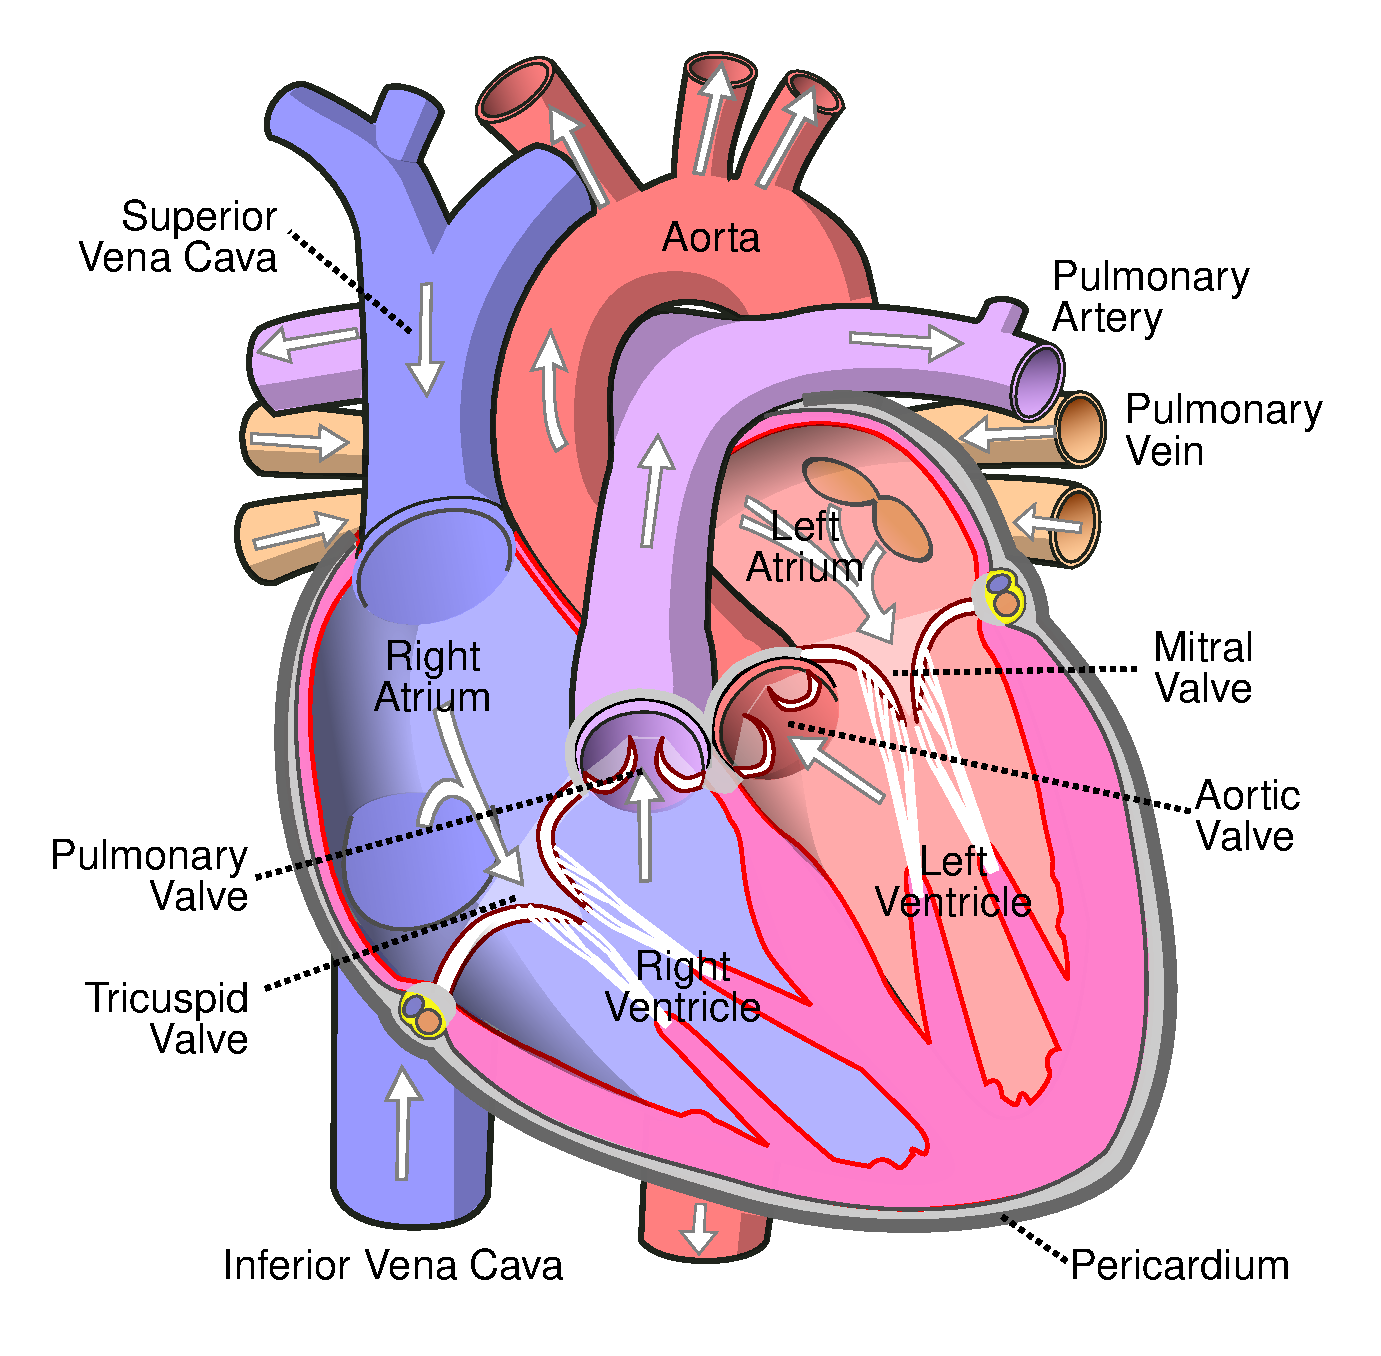
\includegraphics[width=\linewidth]{content/background/figures/heart_chambers.pdf}
    \caption{The four chambers, four valves and the direction of flow; the coronary arteries are not drawn. Figure by Wapcaplet, CC BY-SA 3.0, via Wikimedia Commons.}
    \label{fig:heart-chambers}
  \end{minipage}\hfill
  \begin{minipage}[t]{0.54\textwidth}
    \centering
    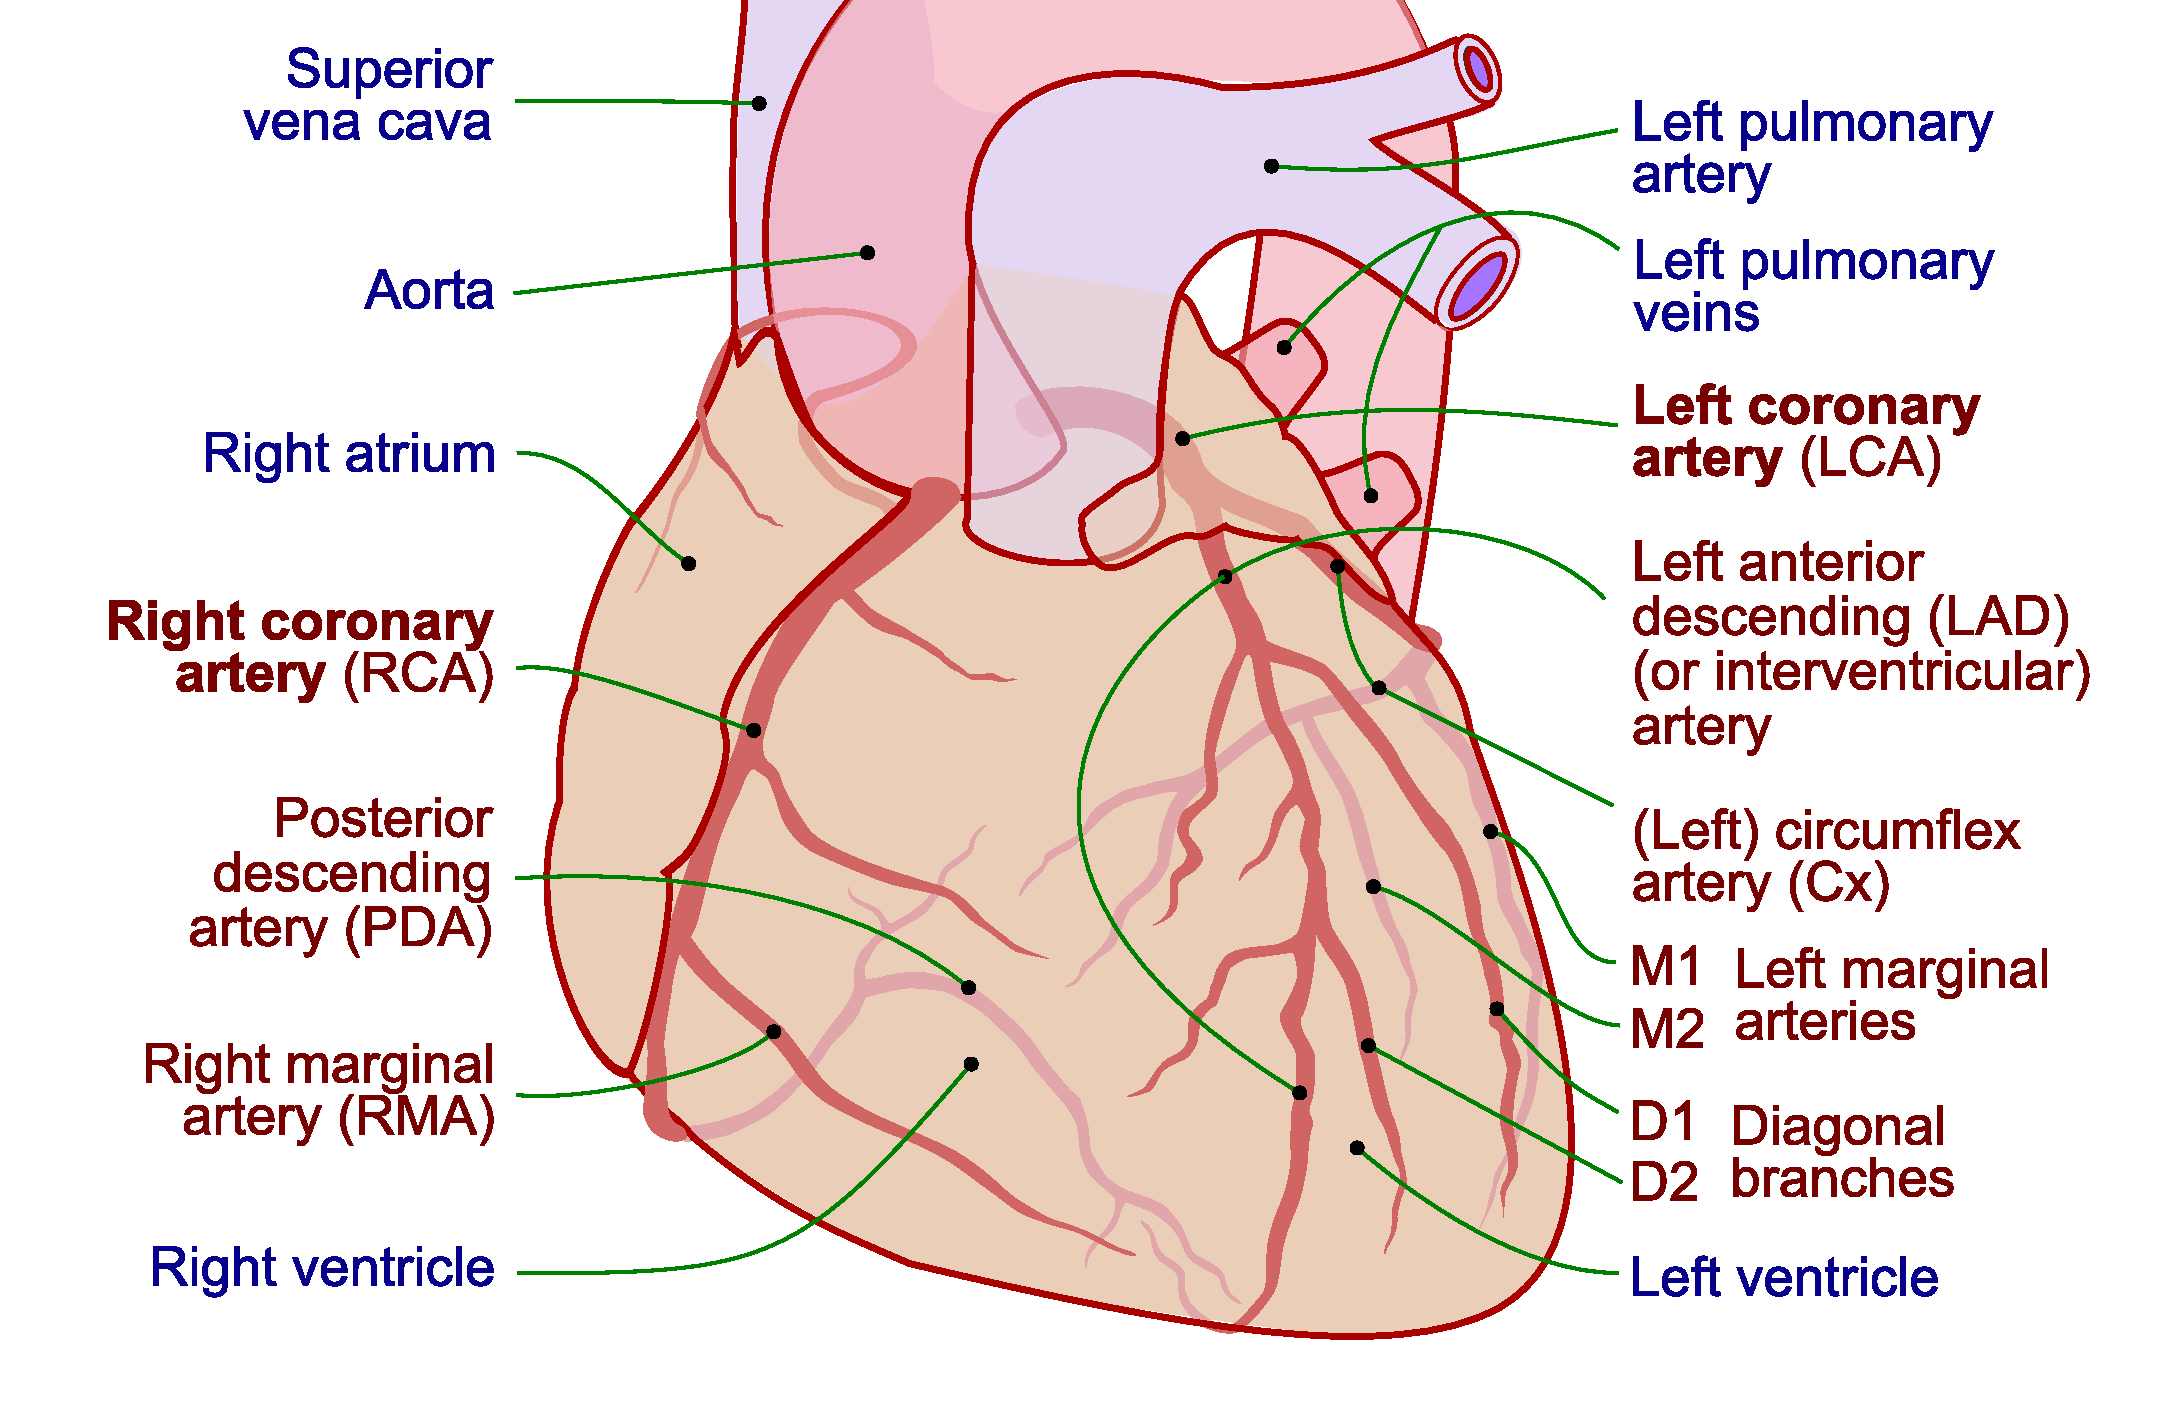
\includegraphics[width=\linewidth]{content/background/figures/coronary_arteries.pdf}
    \caption{The named arteries of both systems, on the surface of the heart, viewed anteriorly.  Figure by Patrick J. Lynch, medical illustrator, via Wikimedia Commons.}
    \label{fig:coronary-arteries}
  \end{minipage}
\end{figure}

\subsection{The coronary arterial tree}
\label{sec:tree}

The left tree begins with the left main artery (LM), leaving the aorta and quickly bifurcating into the left anterior descending artery (LAD) and the left circumflex artery (LCX) (Figure~\ref{fig:coronary-arteries}).
The LAD runs down the front of the heart in the anterior interventricular groove, supplying the front wall of both ventricles \cite{devos2024coronary,obrien2007anatomy}.
The LCX turns the other way along the left atrioventricular groove, supplying the side wall of the left ventricle \cite{obrien2007anatomy,allwork1987applied}.
The LAD sends diagonal branches across the front wall, and the LCX sends obtuse marginal branches over the side wall \cite{devos2024coronary,obrien2007anatomy}.

The right tree begins with the right coronary artery (RCA), which follows the right atrioventricular groove around the other side of the heart \cite{devos2024coronary,obrien2007anatomy}.
On the underside of the heart the RCA usually divides into the posterior descending artery (PDA), which runs forward in the posterior interventricular groove, and the posterior lateral arteries (PLA), which supply the underside of the left ventricle \cite{devos2024coronary,obrien2007anatomy}.

\subsection{Coronary dominance}
\label{sec:dominance}

The point on the underside of the heart where the atrioventricular and interventricular grooves meet is referred to as the crux \cite{allwork1987applied}.
Dominance names the artery that reaches it: a heart is right-dominant when the PDA comes from the RCA, left-dominant when it comes from the LCX, and codominant when the PDA comes from the RCA but the PLA from the LCX \cite{devos2024coronary,allwork1987applied}.
Right dominance is the usual pattern, at 87\% to 96\% across ancestry groups \cite{ihdayhid2021ethnic}.

Dominance changes the size of the arteries as well as which branches they carry: the proximal RCA measures 3.9\,mm in right-dominant and 2.8\,mm in left-dominant hearts, and the LCX 3.4\,mm and 4.2\,mm \cite{dodge1992diameter}.
Branch counts and vessel sizes are therefore comparable only within a dominance group, so every population statistic in this thesis is stratified by dominance.

% Clinical Background v2, section 2. Source: clinical_background/02_cad.tex, rewritten.
% Tone follows the original clinical_background/ (short plain sentences, mechanism told in order),
% as requested 2026-10-05. Cut: unsourced "far more dangerous" and "dies within minutes".
% Headline number from stark2025gbd (supersedes lindstrom2022global).
% 2026-10-05: shortened against Aida's Ch. 2 (style_guide_clinical_aida.md): foam cells, fibrous cap,
% calcification and oxygen extraction cut as unused later; appositive glosses moved to own clauses.
% CHECK: the remaining atherosclerosis sentences are cited to libby2019atherosclerosis, whose full text
% is paywalled and was not opened (refs.bib marks it [PARTIAL]). Verify before submission.
% CHECK: the endothelium-responds-to-flow sentence is now cited to chatzizisis2007ess; confirm it fits.
% CITATION WANTED: the calcium score is recorded for Model 0 (risk_model_plan.tex) but no calcium
% source is in refs.bib; add one before describing it in prose. Not mentioned here for that reason.
% FIGURE: figures/external/atherosclerosis_nhlbi.png (NHLBI, public domain, via Wikimedia Commons), credit
% copied from figures/external/CREDITS.md. Replaced jebari2022_fig3.jpg 2026-10-05 as too detailed. Original is
% only 450x451, so it is printed at half width; rupture is no longer illustrated.

\section{Coronary artery disease}
\label{sec:disease}


Coronary artery disease (CAD) is caused by atherosclerosis, the gradual accumulation of fat and calcium within the walls of the arteries that supply the myocardium, and the resulting deposit is referred to as a plaque \cite{libby2019atherosclerosis}.

The inner wall of every artery is lined by a single layer of cells, referred to as the endothelium.
Plaque formation begins when this layer becomes permeable, so that cholesterol-carrying particles from the blood pass into the wall and accumulate there \cite{libby2019atherosclerosis}.
As the plaque grows, it bulges into the vessel and narrows the open channel through which the blood flows, referred to as the lumen (Figure~\ref{fig:atherosclerosis}) \cite{libby2019atherosclerosis}.

The coronary arteries are the only blood supply of the heart muscle (Section~\ref{sec:circulation}), so a plaque in them impairs cardiac function.
It does so through the following two mechanisms.
The first is gradual: a narrowed artery cannot increase its flow when the heart works harder, leaving the muscle beyond it short of oxygen, a state referred to as ischemia \cite{duncker2015regulation}.
The second is abrupt: a mature plaque has a fatty core covered by a fibrous cap, and when this cap tears, a clot, referred to as a thrombus, forms at the tear and can block the vessel \cite{libby2019atherosclerosis,rampidis2022geometry}.
The muscle beyond a blocked artery loses its oxygen supply, resulting in a myocardial infarction, commonly referred to as a heart attack.

\begin{figure}[h]
  \centering
  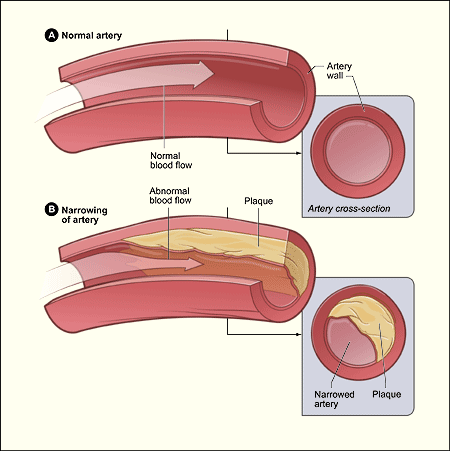
\includegraphics[width=0.5\textwidth]{content/background/figures/atherosclerosis_nhlbi.png}
  \caption{Plaque grows inside the artery wall and narrows the lumen. (A) A healthy artery and its
    cross-section. (B) An artery whose wall holds plaque, with the narrowed lumen shown in
    cross-section. Figure by NHLBI, public domain, via Wikimedia Commons.}
  \label{fig:atherosclerosis}
\end{figure}


% Clinical Background v2, section 3. Source: clinical_background/04_hemodynamics.tex, WSS part only.
% FFR is dropped: the thesis does not predict or use it, and "FFR-UNet" must never be described as
% an FFR estimator (models/ffr_unet.py).
% Tightened to Aida's clinical register (style_guide_clinical_aida.md): mechanism only, citations as
% brackets, no per-study n. The studies themselves live in the literature review
% (asakura1990flow, vandergiessen2009bifurcation, han2022plaque); samady2011wss and yamamoto2017ess
% are n = 20 patients each and partly circular (the plaque deforms the lumen the shear is computed
% from), so they back the mechanism here and nothing more.
% Figure: the two WSS surface maps from Shen 2026 Fig. 6 panels a-b (figures/external/shen2026_fig6.png,
% CC BY 4.0), cropped with trim (in bp = pixels, the PNG has no DPI); streamlines and the secondary-flow inset dropped. No color bar in the original.
% 2026-10-05: bend/bifurcation paragraph rewritten per reports/Low WSS at bends and bifurcations.md.
% chatzizisis2007ess (full text) names both sites but gives no mechanism, so it now backs only the
% opening sentence. zarins1983carotid is carotid: mechanism only. iwami, nakazawa, qiu and zarins
% read at abstract level; quote no numbers from them. Style pass (style_guide_clinical_aida.md): split
% into a bend and a bifurcation paragraph (one structure per paragraph, "In contrast"), flow divider
% and lateral wall named in their own sentence / trailing clause, plaque cites capped at four
% (kimura1996atheroma dropped; its refs.bib entry is kept).
% 2026-10-05: second pass against style_guide_clinical_aida.md (equation block with units, gloss as
% trailing clause, relevance closure). Cut as already covered in 02_disease.tex: the fibrous cap,
% fatty core and rupture mechanism; plaque, endothelium and lumen are used, not redefined.
% Cut as unused later: the 1.5 Pa / 0.4 Pa thresholds (malek1999shear) and the units, since the thesis
% never computes WSS in Pa. Kept: the R^3 dependence, used by the daughter-ratio and Huo-Kassab features.
% 2026-10-05: added subsection sec:wss-mechanism (how low and oscillatory WSS makes the wall
% plaque-prone) on request. Its endothelial claims come from chiu2011disturbed, full text read
% (PMC3844671): cell shape and alignment, turnover and leaky junctions, LDL permeability at branch
% points, eNOS/NO loss, ROS -> NF-kB -> adhesion molecules -> monocyte adhesion, near-wall residence
% time. davies2009shear is abstract-level and backs only the mechanotransduction sentence. Molecule
% names (NF-kB, VCAM-1, ICAM-1, KLF2) kept out as unused later. The oscillatory definition moved up
% from the sites paragraph so the term is defined before its first use.
% 2026-10-05: restructured for flow against style_guide_clinical_aida.md, claims and cite keys unchanged.
% The velocity-gradient sentence moved up to the definition; "branches and bends" now explained only
% in sec:wss-sites; the repeated "fastest blood toward the outer wall" sentence cut; undefined "skew"
% replaced; fragment sentences merged; mechanism subsection cut from five paragraphs to three.
% 2026-10-05: mechanism subsection condensed to two paragraphs on request; cut LDL, reactive
% oxygen species, the monocyte name and the near-wall residence-time point (all still in chiu2011disturbed).
% 2026-10-05: subsections sec:wss-mechanism and sec:wss-sites removed, section renamed "Wall shear
% stress and plaque formation"; restatements of the opening and of 02_disease.tex cut. iwami1998curvature
% and malek1999shear no longer cited.
% 2026-10-05: on request, low-WSS threshold (0.4 Pa / 1.5 Pa, malek1999shear abstract; 0.4 Pa as used by
% kashyap2022tortuosity) and units restored; bend paragraph now explains the circumferential split (symmetric
% profile in a straight tube, inertia skews it in a bend, ku1997blood p.407 + dean1927curved). qiu2000compliant
% number is from its abstract (model, no patients).
% 2026-10-05: reordered for flow: definition, low/oscillatory, where (straight vs disturbed, bend,
% bifurcation), why (endothelium), then the risk closure.

% 2026-10-07: on request, cut the Poiseuille equation and the velocity-gradient lines; the methodology
% (07_daughter_ratio.tex) no longer leans on the R^3 law. New order: definition, low WSS -> plaque, why
% (endothelium), where (bend, bifurcation), geometry predicts low WSS (kashyap2022tortuosity: CAD-free
% CTCA; garcha2025sensitivity: synthetic), geometry-derived WSS predicts as well as CFD (griffo2026wss).
% 2026-10-07: endothelium paragraph cut from five sentences to four; "mechanotransduction" and
% "endothelial dysfunction" dropped as used nowhere else, cell turnover/junction detail dropped.
% CAREFUL on griffo: endpoint is future-culprit vs non-culprit lesions within MI patients, AUC 0.63 for
% both arms, angiography not CCTA. Do not upgrade it to "predicts plaque" or "predicts risk".
\section{Wall shear stress and plaque formation}
\label{sec:wss}

Blood flowing along an artery exerts a frictional force on the vessel wall, referred to as the wall shear stress (WSS).
Plaque forms and grows preferentially where the WSS is low or oscillatory, meaning that it reverses direction over the cardiac cycle \cite{chatzizisis2007ess,samady2011wss,yamamoto2017ess}.
High WSS, in contrast, is harmful only to plaque that already narrows the vessel, where it increases the risk of rupture \cite{bajraktari2021highwss,samady2011wss}.

The link between WSS and plaque runs through the endothelial cells that line the vessel, which sense the WSS and respond to it \cite{davies2009shear}.
Where the WSS is high and unidirectional, these cells release nitric oxide, which protects the wall \cite{chiu2011disturbed}.
Where it is low or oscillatory, they release less, so the endothelium becomes leaky and inflamed \cite{chiu2011disturbed}.
Cholesterol-carrying particles and white blood cells then pass into the wall, and plaque begins to form (Section~\ref{sec:disease}) \cite{chiu2011disturbed}.

In a straight segment, the blood flows forward throughout the cardiac cycle and the velocity profile is symmetric about the center, so the WSS is high, unidirectional and the same all around the wall \cite{chiu2011disturbed}.
In a bend, this symmetry is lost: the blood tends to keep moving in a straight line, so the fastest-moving blood is carried toward the outer wall \cite{ku1997blood,dean1927curved}.
The velocity therefore rises steeply from the outer wall and gently from the inner wall, so the same cross-section has high WSS on its outer side and low WSS on its inner side (Figure~\ref{fig:wss-sites}) \cite{ku1997blood,qiu2000compliant}.
In a model of a coronary bend, the mean WSS on the inner wall was about half that on the outer wall, and it oscillated more over the cardiac cycle \cite{qiu2000compliant}.
This slow, reversing flow along the inner wall is referred to as disturbed flow, and it grows stronger the tighter the bend and the higher the flow rate \cite{chiu2011disturbed,ku1997blood}.

At a bifurcation, the parent vessel splits at a ridge, referred to as the flow divider.
The fastest-moving blood continues onto the flow divider, where the WSS is high \cite{zarins1983carotid,antoniadis2015bifurcation}.
In contrast, the flow is disturbed along the lateral walls, the walls of the daughter branches that face away from the flow divider \cite{asakura1990flow,antoniadis2015bifurcation}.
The extent of this region depends mainly on the share of the parent flow that enters the side branch \cite{antoniadis2015bifurcation}.
The flow divider is largely spared from plaque \cite{asakura1990flow,vandergiessen2009bifurcation,nakazawa2010pathological}.


% Clinical Background v2, section 4. Source: clinical_background/03_ccta.tex.
% Fixed: CCTA expanded at first use; resolution claims now sourced (dodge1992diameter,
% medranogracia2016atlas); our 0.5 mm grid stated.
% SINGLE SOURCE: abbara2016scct still carries gating and motion. A second source is wanted;
% nieman2024scct is in refs.bib but its full text is not read, so it is not cited here.
% FIGURE WANTED: acquisition schematic, or a clean vessel beside one degraded by motion and
% blooming. External figure needs a credit from figures/external/CREDITS.md. No \ref until it exists.
% CHECK: that the segmentation network of this thesis is run on the 0.5 mm resampled volumes is a
% pipeline fact (CLAUDE.md, volumes_resampled/), stated without citation.

\section{Coronary CT angiography}
\label{sec:ccta}

Coronary computed tomography angiography (CCTA) is the non-invasive imaging test recommended as the first-line investigation in patients with suspected chronic coronary syndrome \cite{knuuti2019esc}.
During acquisition, the patient lies on the table of a computed tomography scanner, and a contrast agent, a solution containing iodine that absorbs X-rays strongly, is injected into a vein in the arm.
The X-ray tube and its detector rotate around the patient, recording a projection of the chest at each angle, and the projections are reconstructed into a three-dimensional volume \cite{abbara2016scct}.
The acquisition is timed to the passage of the contrast agent through the coronary arteries, resulting in a volume in which the lumen appears bright against the surrounding tissue \cite{abbara2016scct}.

As the coronary arteries move with the heart muscle throughout the cardiac cycle, acquisition is synchronized to the electrocardiogram, and the volume is reconstructed from the phase of least motion, conventionally mid-diastole \cite{abbara2016scct}.
The heart rate is lowered with medication before the scan, lengthening this window \cite{abbara2016scct}.The reconstructed volume is a grid of voxels, the three-dimensional equivalent of pixels, and no structure smaller than a voxel can be resolved.
% Technical Background -- chapter opening. Section files are included in numeric order from
% content/background.tex. Moved 2026-11-07 from thesis/technical_background/00_chapter_intro.tex.
% Written to thesis/style_guide_technical_aida.md (after Aida's Chapter 3).
% Rule for what belongs here: a sentence that would be true if this thesis had never been written is
% background; what was done, with which settings, on which data, is Methodology. Every section is
% pointed back to by a Methodology section (content/methodology/0*.tex); if none does, cut it.
% Sections:
%   01_prediction_model.tex   cloglog GLMM written 2026-11-13 (risk models,     sec:tech-model
%                             recalibration, bootstrap still notes)
%   02_fpca.tex               functional principal component analysis, written sec:tech-fpca
%   01b_sample_size.tex       Riley criteria for a binary outcome (2026-11-10)   sec:tech-sample-size
% Not written yet, on purpose, until the model is confirmed: added predictive value (was
%   thesis/technical_background/03_added_value.tex).
% Map, Methodology file -> background it relies on:
%   03_prediction_model      sec 1
%   04_model_size            sec 1b (Riley criteria)
%   07_curvature_fpca        sec 2 (cut sec 2 if the descriptive FPCA is dropped)
% Each definition lives once: here if it is general, in the Methodology if it carries a setting.
% No opening paragraph and no roadmap: Aida's chapter starts directly at its first section.
% Present tense; past only for history (introduced in ...). No settings, no cohort, no results.

\chapter{Technical Background}
\label{ch:technical}


% The one Technical Background file that describes the prediction model.
% Trimmed 2026-11-07 from thesis/technical_background/01_risk_models.tex, 02_segment_glmm.tex and
% the reserve 02_segment_glmm_long.tex (full drafts in git, commit e4eb857).
% 2026-11-13 (user: "use the pooled cloglog GLMM evaluation to write the technical section; style of
%   fpca.tex first half; flow between the lines"). WRITTEN: the GLMM part only (scope chosen with the
%   user; risk models, recalibration and the general bootstrap are still NOTES below, because the base
%   choice, recalibrated vs refitted SCORE2, is open). 4 displayed equations (eq:tech-glmm,
%   eq:tech-lr, eq:tech-agg-conditional, eq:tech-agg-marginal). Source: reports/Pooled cloglog GLMM
%   evaluation.md, on top of the retired outdated/thesis_retired/technical_background/02_segment_glmm.tex.
%   Argument changed from the retired draft: the random intercept is justified by valid standard errors
%   and a joint distribution, NOT by better prediction; "slope 0.79 vs 0.98" dropped (logit, ICC 0.30,
%   not the size here); cloglog is the grouped-time form of a PH frailty model; log exposure with a
%   free coefficient and the offset as the special case; variance weakly identified in small binary
%   clusters; LR test needs the random intercept to capture the dependence; the independence product
%   overstates the cluster risk. Generic wording on purpose ("unit", "cluster", "exposure"): the
%   segments, persons, log length and the nine segments are Methodology. Notation: H_i (summed
%   hazard, not S_i, taken by the shrinkage in 01b_sample_size.tex), q (block size, not k), f(b;
%   sigma^2) for the normal density (phi is the FPCA eigenfunction).
%   Not cited on purpose (individual studies, Lit. Review or Discussion): Lingsma 2013, Bouwmeester
%   2013, Falconieri 2020, TRIPOD-Cluster, the coronary cohort papers, Riley.
%   2026-11-13 (counterfactual rule): GEE cut from the opener. Removed: "Marginal models such as GEE
%     estimate the average effect across clusters and correct the SEs without describing the
%     correlation (liang1986gee)" and "for a new cluster, predictions about as accurate as a marginal
%     model once b is integrated out (pavlou2015marginal)". The real case for GLMM over GEE is the
%     joint distribution needed for the cluster risk (sec:tech-aggregation); GEE SEs survive a wrong
%     working correlation, GLMM SEs and the LR test do not. For the examiner and, if the artery-level
%     dependence is raised, one line in the Discussion. liang1986gee is now uncited.
%   CHECK: pavlou2015marginal is cited for "predictions about as accurate as a marginal model once
%     integrated" (report: opened via a summarising tool, logit simulations); confirm in the PDF.
%   CHECK: moineddin2007multilevel and austin2010clusters, same (poor variance estimates, small
%     binary clusters; regimes are 5-100 clusters, not ~1000 clusters of nine).
%   CHECK: prentice1978grouped, duchateau2008frailty (chapter and page), liu1994gausshermite,
%     pinheiro1995approximations, joe2008laplace were not read in full; the unread ones are cited for
%     standard results (grouped PH gives cloglog; shared frailty; adaptive quadrature; Laplace bias).
%   CHECK: "the test then rejects too often" and "the independence product overstates" are reasoning,
%     uncited; the report grades them as inference.
%   Pointed back to (labels): sec:tech-segment-glmm, sec:tech-glmm-likelihood, sec:tech-aggregation,
%     eq:tech-lr, sec:tech-nested (methodology/03_prediction_model.tex notes).
% 2026-11-13: added sec:tech-nested (nested random intercepts, eq:tech-nested, eq:tech-nested-icc) for
%   the three-level sensitivity analysis (person + artery within person; mapping is Methodology).
%   Notation: subgroup g(j) keeps y_ij/eta_ij; omega^2 (tau is the taper, k the coefficient index).
%   Boundary LR test cites self1987boundary, stram1994variance [TO VERIFY]. Latent variance pi^2/6
%   has a \todonote until a source is read. sec:tech-aggregation still assumes one intercept: fine
%   while the sensitivity analysis reports only variances, LR test and hazard ratios; extend it only
%   if person risk is computed under the nested model.
%   CHECK: file spelling is American (summarized, neighboring) against the British rule in CLAUDE.md;
%   new text follows the file ("unmodelled" is the one British form); sweep later.
% Added value (C, calibration, Brier, log loss, NRI/IDI, internal validation; was 03_added_value.tex)
%   is deliberately not written yet.
% Pointed back to by: content/methodology/03_prediction_model.tex (sec:method-models).
% Rule: general methods only, present tense; settings, covariates, software and node counts are
% Methodology.
%
% The section should contain, whatever the model:
% - Clinical risk prediction models: absolute risk of an outcome over a time horizon from
%   predictors, linear predictor mapped to a risk through a link (steyerberg2019cpm). Weights set
%   the ranking, the intercept the level.
% - Developed in the data versus a published score; SCORE2 (score2_2021) as the example. A published
%   score costs no parameters but its weights were chosen for its own outcome and population.
% - Recalibration (janssen2008updating, cox1958binary): in-the-large, logistic recalibration
%   (intercept + one slope on the published linear predictor), revision, refitting; each step costs
%   more parameters. Recovering the linear predictor from a published risk on the link scale.
% - Hazard closer: a recalibrated score keeps its relative weights, so a new block correlated with a
%   mis-weighted factor (e.g. age) can look informative only by correcting that weight. Does NOT
%   decide the open base choice (recalibrated SCORE2 vs refitted factors).
%
% - The bootstrap in general (added 2026-11-09): resampling the observations (here persons) with
%   replacement to see how an estimate would vary across samples; percentile intervals. Used twice
%   in the thesis: the person-level bootstrap for the intervals of the model's estimated measures
%   (Methods 03 notes; plan in ~/Desktop/Speciale/CGPS_statistics-/CLAUDE.md) and the stability
%   check of the FPCA components (sec:tech-fpca-components, Methods 07). Explain it once here so
%   the FPCA section can point back. CITATION WANTED: a classic source (e.g. Efron and Tibshirani
%   1993, An Introduction to the Bootstrap); not yet in refs.bib, add and check before citing.
%
% If the cloglog GLMM is confirmed, it should also contain:
% (Updated 2026-11-11 from reports/Pooled cloglog GLMM evaluation.md. Its verdict: keep the model,
% change the argument for it. No non-ML alternative was found that is clearly better.)
% - Clustered binary outcomes (segments within persons); correlated outcomes make naive standard
%   errors too small; GLMM adds a random person effect (statacorp2025mecloglog). Practice: only
%   5 of 15 intracoronary imaging studies with several observations per patient handled clustering
%   (Lingsma 2013 EuroIntervention, NOT IN refs.bib); coronary cohort papers mostly use GEE or
%   marginal Cox with robust variance, so say why a GLMM rather than GEE (see "why a GLMM" below).
% - WHY A GLMM (the justification to write; replaces any "predicts better" claim): a random
%   intercept does NOT predict better for a new person. Integrated predictions tie with GEE and
%   standard logistic (calibration slopes 0.97-0.98, pavlou2015marginal); b = 0 is worse
%   (Bouwmeester 2013, NOT IN refs.bib). The model earns its place for two other reasons: (1)
%   honest standard errors, so a valid LR test of the geometry block; (2) a joint model of the
%   segments, which is what lets segment risks be combined into a person risk. GEE gives only
%   marginal segment risks, and the independence product 1 - prod(1 - p) overstates the person
%   risk under positive within-person correlation.
% - Cloglog link: proportional hazards over the window give hazard ratios independent of window
%   length (prentice1978grouped); logit gives odds ratios, close at low risk. Say honestly that fit
%   cannot tell the links apart at segment level; the reason for cloglog is interpretive (hazard
%   ratios, segment hazards add to a person hazard). The link does matter for the person risk,
%   which is not small (check the event rate, see below).
% - Survival reading (use as justification): with two scans each segment has one interval, so an
%   interval-censored shared-frailty PH model collapses to this GLMM: the two-scan, discrete-time
%   counterpart of the shared-frailty Cox model that lesion-level studies already accept. Log
%   follow-up as an offset = constant baseline hazard; free coefficient = Weibull baseline
%   (standard result, VERIFY in prentice1978grouped before writing). PH cannot be tested with one
%   follow-up scan; say so.
% - Exposure such as segment length: log length as an offset (coefficient 1) assumes hazard
%   proportional to length, with no coronary precedent found. Present the free coefficient as the
%   default (1 df, interval reported against 1) and the offset as the special case. Curvature and
%   taper are computed per segment and depend on length, so a wrong offset can leak into the
%   tested block.
% - Random intercept: shared frailty multiplying all segment hazards (duchateau2008frailty, page
%   still to verify), summarised by sigma^2; conditional versus marginal effects
%   (pavlou2015marginal); median hazard ratio (austin2017mhr). Weak point to state: sigma^2 is
%   informed almost only by persons with two or more positive segments, and small binary clusters
%   bias variance estimates (Moineddin 2007, Austin 2010, NOT IN refs.bib; their regimes are 5-100
%   clusters, not ~1000 clusters of nine, so the size of the bias here is unknown). Robustness to
%   a non-normal random effect holds for slopes, not for variance components or the person risk.
% - Fitting and testing: integration over the random intercept by adaptive Gauss-Hermite quadrature
%   (liu1994gausshermite); Laplace bias in small binary clusters (joe2008laplace), so Laplace is
%   never the primary fit; LR test of a block of k coefficients against chi^2_k, both models on
%   the same rows and settings. The chi^2 reference is asymptotic; a parametric bootstrap of the
%   LR statistic checks it, but only under the fitted model (it does not protect against
%   dependence beyond one shared intercept; a person-cluster bootstrap or robust Wald test does).
% - Segment risk to person risk: given b_i the segment hazards add (S_i), and the person risk
%   integrates over b; b_i = 0 gives the median person and is miscalibrated. Do NOT quote
%   pavlou2015marginal's "slope 0.79 vs 0.98" as the expected size here: it is a logit result for
%   individual predictions at ICC 0.30. Use it for the direction only; the size is computed in the
%   cohort (Methods). The person risk depends on sigma^2 and on the assumed normal shape, which
%   segment-level fit and the C-statistic cannot see; only person-level calibration can. An effect
%   on one segment is diluted in S_i, so a rejected LR test need not change the person risk.
% - Sample size: Riley criteria (riley2019) assume independent observations and are silent on
%   clustering. Count persons and person-level events, never segment rows (three of the five
%   geometry features are person-level constants, so segment rows are pseudo-replicates for
%   them). Shrinkage of the pooled model is estimated by resampling, not asserted from the formula.
% - TRIPOD-Cluster (Debray 2023, NOT IN refs.bib) explicitly puts clustering within individuals
%   out of scope; cite it by analogy only: state how clustering was handled, which intercept the
%   predictions use, and keep every model-building step inside the resampling.
%
% Belongs in Methodology 03, not here (recorded so it is not lost; general method only above):
% - Base model: free coefficient on log length; integrated person risk stated explicitly, b = 0 and
%   the independence product not used; the b = 0 error computed in the cohort.
% - Decide which rows carry the three left-main features (now pLAD and pLCx, adjacent rows) before
%   the test is locked; put a person-level test of those three features beside the block test.
% - Before locking: tabulate the segment-level event rate and the number of persons with two or
%   more positive segments (they decide how well sigma^2 is identified). The research notes
%   assumed rare events; the earlier report gives ~452 of 1,076 persons with new plaque (~42%),
%   NOT verified against current data.
% - Prespecified sensitivity analyses, in order of value: (1) person-level cloglog on per-person
%   geometry summaries (benchmark; tests "who"); (2) working-independence cloglog GEE with a
%   robust 5-df Wald test plus person-cluster bootstrap; (3) parametric bootstrap of the LR
%   statistic; (4) gamma-frailty refit (closed-form person risk); (5) fold-wise sigma-hat from
%   several starts, boundary estimates reported; (6) logit refit and fixed-offset length; (7)
%   person means of curvature and taper (+2 df, between-within); (8) number of evaluable segments
%   as covariate, calibration by segment count; (9) observed vs model-implied plaque
%   co-occurrence in adjacent and non-adjacent segment pairs; (10) vessel-within-person intercept.
% - Dependence beyond one shared intercept (added 2026-11-11, from talk prep). The single b_i
%   gives every pair of segments the same latent dependence, but real dependence likely follows
%   the tree: parent-child along a vessel (proximal -> mid -> distal) and the two left-main
%   daughters (pLAD-pLCx), which also carry the same left-main feature values. If so, those rows
%   count as more independent evidence than they are and the LR test is anticonservative. Do NOT
%   add the vessel intercept (10) to the primary model: it is a second variance, informed only by
%   persons with >= 2 positives in the same vessel, so it will likely sit at the boundary; keep
%   it as a sensitivity fit. Check the assumption without spending parameters instead:
%   (a) Co-occurrence check (9): compare how often a pair of segments is both positive in the
%       data with how often the fitted model predicts it, separately for parent-child pairs, the
%       pLAD-pLCx siblings and pairs in different vessels. Uses b: the model-implied joint
%       probability is P(Y_j = 1, Y_k = 1) = integral of p_j(b) p_k(b) N(b; 0, sigma^2) db, the
%       segments being independent only given b. If observed and predicted agree, the single
%       sigma^2 is adequate.
%   (b) Person-cluster bootstrap or GEE robust Wald test (2): valid for the geometry block
%       whatever the true dependence (tree-shaped, sibling or other), without modelling it. If
%       they agree with the LR test, the result holds. The cluster bootstrap resamples whole
%       persons and refits the GLMM, so it still uses b. The GEE has no b: it is a marginal
%       (population-averaged) model with working independence and sandwich standard errors, so
%       its coefficients are on a different (attenuated) scale from the GLMM's conditional ones;
%       compare the tests (geometry block = 0), not the coefficient sizes.
% - Optional: a short simulation at the fitted base-model parameters (sigma-hat = 0 rate, type I
%   error of LR and robust Wald for a 5-df block, person-level calibration under normal and
%   non-normal frailty). No published simulation covers this data shape.
% - Rejected alternatives, one line each in the Discussion: penalised (ridge/lasso/Firth) GLMM
%   (unreliable at small effective n, loses the LR test; Riley 2021), Bayesian GLMM (equal at
%   best), beta-binomial (cannot hold segment covariates), conditional logistic (drops persons
%   without events and all person-level features), random slopes and spatial effects (not
%   estimable with nine rows).
% - Examiner checklist: GLMM vs GEE; cloglog vs logit; length as exposure and whether fixed;
%   conditional vs marginal and which prediction is evaluated; the aggregation assumption;
%   resampling by person including every estimated quantity; quadrature settings; how a sample-size
%   criterion for independent persons was applied to a model fitted on segment rows.
% - CHECK BEFORE CITING: every number above was relayed by a summarising tool; check against the
%   PDFs. Full list of abstract-only and snippet-only sources in the report's last section.
% 2026-11-13 (user: "only the most important, 2-3 pages; human phrasing after the Aida style guide,
%   not a math book; easy on the first read; concise"). Rewritten from about 1,500 to about 900 prose
%   words, 6 to 5 displayed equations, 4 to 3 subsections. Copy before this pass: scratchpad
%   01_prediction_model_before_short.tex (not in the repo). Claims, cite keys and kept labels unchanged.
%   - FOLDED (user): sec:tech-nested is now one paragraph inside sec:tech-segment-glmm (label kept on
%     the paragraph, so a reference gives that subsection's number). eq:tech-nested kept.
%   - CUT: eq:tech-nested-icc (latent correlations rho_same, rho_different) and its pi^2/6 todonote
%     (no source read); nothing referenced the label. Restore from git if the Methodology needs ICCs.
%   - CUT: "the logit odds ratios change with the baseline risk"; the cost of nested quadrature
%     ("grows with the square of the number of nodes"); the dilution algebra (H_i multiplied by
%     (1 - w) + wh, w the unit's share), now said in words; "attenuated toward zero" -> "smaller".
%   - Boundary test reduced to one sentence (self1987boundary, stram1994variance [TO VERIFY]).
%   - Spelling now British in the prose (generalised, summarised, maximised); heading kept as
%     "Generalized" until the whole-thesis spelling sweep.
% 2026-11-13 (second pass, user: "look at how Aida explains mathematical components; not static and
%   academic; human-written; go through the entire text"). Aida's pattern applied: assumptions in
%   words first ("Under these assumptions, ..."), then the equation, then the symbols in a "where"
%   clause after it; no symbol defined before the reader knows why it is needed (the opening "Let
%   y_ij be 1 if ... and let eta_ij be ..." is gone). Each step of the chain says what it adds ("So
%   far the units are treated as independent"). NEW: one unnumbered display for the model without
%   the cluster effect, so eq:tech-glmm reads as one added term. y_ij no longer named in the text;
%   A_i is defined in words in sec:tech-aggregation. Claims, cites and labels unchanged.
% 2026-11-13 (third pass, user: "make the technical background more human"): light touch only, the
%   section was already rewritten for tone twice today. "Its main appeal is the reading of" -> "that
%   the coefficients are easy to read:"; "fit nearly alike" -> "give nearly the same fit"; "Since"
%   opener removed; ambiguous "It ranks" -> "This shortcut ranks"; dilution closer reworded.
% 2026-11-13 (user): first display rewritten so the hazard ratio is visible in it: Lambda_ij (hazard
%   accumulated over the window) = exp(eta_ij), eta_ij = beta_0 + sum_k beta_k x_ijk (was x^T beta,
%   with beta_k never defined). Link written out; why window-independence matters added. Later
%   displays unchanged: exp(eta_ij + b_i) is Lambda with the cluster effect, and H_i in
%   sec:tech-aggregation is the sum of the Lambda_ij.
% 2026-11-13 (user: better openings, collapse sections): subsection "The Complementary Log-Log Model"
%   removed, so the section runs from the clustering problem straight into the model; its label
%   sec:tech-segment-glmm now sits on the paragraph (nothing outside this file references it).
%   Openers: "Some units have more room ..." -> "Units also differ in how much opportunity ...";
%   "So far the units are treated as independent." -> "The model above still treats every unit on
%   its own. To let the units of a cluster share their risk, ..." (", shared by all units of
%   cluster i," inserted clause removed). Two subsections remain: Fitting and Testing; From Unit
%   Risk to Cluster Risk.
% 2026-11-13 (user, /plan: "The Complementary Log-Log Model more concise, not as deep where not
%   necessary"): subsection is back in the text and shortened by about a third. CUT: "This matters when
%   the windows differ in length"; the full median-hazard-ratio definition; "b_i not estimated one by
%   one" (merged with sigma^2 = 0); "units in the same subgroup share both effects" (follows from
%   eq:tech-nested); "hazard grows as E^gamma". Claims, cites, equations and labels unchanged.
% 2026-11-13 (user: "infer aida styleguide over the section"; outdated/thesis_retired/
%   style_guide_technical_aida.md + style_guide_aida.md): assumptions named before the first display
%   ("Under the assumptions that ..."); symbols in "where" clauses (sigma^2, omega^2 back there);
%   "event rate, or hazard" synonym pattern; "A key characteristic of this link"; random effect and
%   nested effect open on the limitation they address ("While ...", "A single random effect makes
%   ..."); inserted glosses removed (", the hazard, which", ", an offset,"); participial tail on
%   exposure; sigma^2 hazard closer split into fact + "therefore". Slightly longer than the concise
%   pass, still shorter than the original. Claims, cites, equations and labels unchanged.
% 2026-11-13 (user: "the prediction model cannot be longer than Aida's longest section"): Aida's
%   longest is 3.2 U-Net + 3.2.1 nnU-Net, about 735 words incl. equation fragments (3.3 + 3.3.1
%   about 730). Whole section cut from about 1,260 to under 735 on the same basis. Labels, cites
%   and numbered equations kept. [2026-11-13 later, user: "more academic, keep tone": cloglog opening
%   reworded; assumption named (proportional hazards); "hazard accumulated" -> "cumulative hazard";
%   link written as log{-log(1-p)} = eta; "A key property of this link". Claims and cites unchanged.
%   Then (user: "more human and direct, optimise flow"): plain opener ("either has an event ... or it
%   does not"); assumption as a colon statement; "Rearranging gives"; "Its main advantage";
%   exposure introduced by its reason ("Units also differ in how much opportunity ...").
%   Then (user: "concise, Aida style, no repetition"): "A key characteristic of this link" (Aida 3.3);
%   HR defined per unit increase; exposure via "commonly referred to as"; gamma's role stated as
%   hazard ~ E^gamma; example "such as the size of the unit" dropped (inserted gloss, and the chapter
%   stays generic). No re-mention of cloglog name, PH or window definition.]
%   CUT: logit comparison (counterfactual rule; one line for the
%   Discussion: logit gives odds ratios, near-identical fit when events are rare); exposure as
%   E^gamma; sigma^2 = 0 'no clustering'; 'effects averaged over clusters are smaller'; nested
%   'informed only by subgroups with > 1 event, can come out as zero'; 'more nodes ... closer';
%   'same settings, so the difference comes from the block'; 'nodes raised until estimates stop
%   changing' (a setting, Methodology); nested quadrature sentence; 'integral
%   stays one-dimensional'; 'only calibration can tell them apart' (folded); dilution closer
%   shortened to one sentence; eq:tech-nested display made inline (label dropped, nothing cited it;
%   sec:tech-nested kept). Backup of the pre-cut file: scratchpad 01_prediction_model_before_735.tex.
\section{Generalized Linear Mixed Model}
\label{sec:tech-model}

A generalised linear mixed model (GLMM) is a regression model designed for outcomes observed in clusters, where several units belong to the same cluster.
Units of one cluster share unmeasured traits, so their outcomes tend to occur together, and ignoring this gives standard errors that are too small.
A GLMM adds a random effect for each cluster, keeping the standard errors valid and modelling the dependence within a cluster \cite{statacorp2025mecloglog}.

\subsection{The Complementary Log-Log Model}
\label{sec:tech-segment-glmm}
Each unit is followed over an observation window, and the outcome is whether it has an event.
To link this outcome to the covariates, the model assumes proportional hazards: each covariate scales the event rate by a constant factor throughout the window.
The probability that unit $j$ of cluster $i$ has an event is then given by 
\[
  p_{ij} = 1 - \exp\!\left(-\Lambda_{ij}\right),
  \qquad
  \Lambda_{ij} = \exp(\eta_{ij}),
  \qquad
  \eta_{ij} = \beta_0 + \sum_{k} \beta_k\, x_{ijk},
\]
where $\Lambda_{ij}$ is the hazard summed over the whole window, known as the cumulative hazard, and $\beta_k$ is the coefficient of covariate $x_{ijk}$.
Rearranging shows that the model is linear in the covariates on a transformed scale,
\[
  \log\{-\log(1 - p_{ij})\} = \eta_{ij},
\]
where the left-hand side is the complementary log-log (cloglog) of the event probability.
Increasing $x_{ijk}$ by one unit multiplies the hazard by $\exp(\beta_k)$, which is therefore the hazard ratio of covariate $k$.
The factor applies equally at every moment of the window, so the hazard ratio does not depend on how long the window is \cite{prentice1978grouped}.
Units may also differ in how much opportunity they have for an event, for example because some units are larger than others.
This opportunity is called the exposure, $E_{ij}$, and it enters $\eta_{ij}$ as an additional term $\gamma \log E_{ij}$.
The hazard then grows in proportion to $E_{ij}^{\gamma}$, so that with $\gamma = 1$ doubling the exposure doubles the hazard.
When $\gamma$ is fixed at 1 instead of being estimated, the term is called an offset.

While this model treats every unit on its own, the units of a cluster share part of their risk.
The GLMM captures this by adding a random effect $b_i$ to every unit in cluster $i$,
\begin{equation}
  p_{ij}(b_i) = 1 - \exp\!\left\{-\exp(\eta_{ij} + b_i)\right\},
  \qquad
  b_i \sim \mathcal{N}(0, \sigma^2),
  \label{eq:tech-glmm}
\end{equation}
where $\sigma^2$ is the variance of the cluster effects, often reported as a median hazard ratio \cite{austin2017mhr}.
Given $b_i$ the units are assumed independent, and $e^{b_i}$ multiplies the hazard of every unit in the cluster by the same factor, known as a shared frailty \cite{duchateau2008frailty}.
The coefficients are therefore conditional, comparing two units of the same cluster \cite{pavlou2015marginal}.
Most of the information about $\sigma^2$ comes from clusters with more than one event, so it is estimated poorly when clusters are small and events are few \cite{moineddin2007multilevel, austin2010clusters}.

\label{sec:tech-nested}%
When the units fall into subgroups that share more than the cluster as a whole, a nested random intercept adds a second effect $c_{ig(j)} \sim \mathcal{N}(0, \omega^2)$ for the subgroup $g(j)$ of unit $j$ next to $b_i$ in Eq.~\eqref{eq:tech-glmm}.
Setting $\omega^2 = 0$ gives back the single intercept, and $\omega^2$ is even harder to estimate than $\sigma^2$.

\subsection{Fitting and Testing}
\label{sec:tech-glmm-likelihood}

The cluster effects are not observed, so the likelihood averages over $b_i$, an integral with no closed form.
Adaptive Gauss--Hermite quadrature approximates it by a weighted sum over a few nodes placed around the most likely value of $b_i$ \cite{liu1994gausshermite, pinheiro1995approximations}.
With a single node it reduces to the Laplace approximation, which is biased for binary outcomes in small clusters \cite{joe2008laplace, statacorp2025mecloglog}.

To test whether a block of $q$ covariates adds anything, the model is fitted with and without the block on the same rows,
\begin{equation}
  \mathrm{LR} = 2\left(\ell_1 - \ell_0\right) \;\overset{H_0}{\sim}\; \chi^2_q ,
  \label{eq:tech-lr}
\end{equation}
where $\ell_1$ and $\ell_0$ are the maximised log-likelihoods.
The $\chi^2$ reference holds only if the random effects capture the dependence within a cluster, and otherwise the test rejects too often.
For $\omega^2 = 0$ the p-value of the $\chi^2_1$ test is halved, as a variance cannot be negative \cite{self1987boundary, stram1994variance}.

\subsection{From Unit Risk to Cluster Risk}
\label{sec:tech-aggregation}

The question of interest can be whether any unit of a cluster has an event, written $A_i = 1$.
Given $b_i$ the units are independent, and under the cloglog model the product of their probabilities collapses to a single exponential,
\begin{equation}
  P(A_i = 0 \mid b_i) = \prod_{j=1}^{n_i} \exp\!\left(-e^{\eta_{ij} + b_i}\right)
  = \exp\!\left(-e^{b_i} H_i\right),
  \qquad
  H_i = \sum_{j=1}^{n_i} e^{\eta_{ij}} ,
  \label{eq:tech-agg-conditional}
\end{equation}
where $n_i$ is the number of units and $H_i$ is their summed hazard.
For a new cluster $b_i$ is unknown, so the risk is averaged over its distribution,
\begin{equation}
  P_i = P(A_i = 1) = 1 - \int \exp\!\left(-e^{b} H_i\right) f(b;\sigma^2)\,\mathrm{d}b ,
  \label{eq:tech-agg-marginal}
\end{equation}
where $f(b;\sigma^2)$ is the normal density with mean 0 and variance $\sigma^2$.

Setting $b_i = 0$ instead gives the risk of the median cluster, which ranks the clusters identically but is miscalibrated \cite{pavlou2015marginal, skrondal2009prediction}.
Multiplying the unit risks as if the units were independent overstates the cluster risk when outcomes occur together.
It also depends on $\sigma^2$ and the normal shape of $b_i$, so it is judged by calibration at the cluster level.
An effect on a single unit is diluted in $H_i$, so a block that is significant in Eq.~\eqref{eq:tech-lr} may barely change the cluster risk.

% Technical Background, sample size. Source: outdated/thesis_retired/technical_background/03b_sample_size.tex
% (written 2026-11-06), brought to the register of methodology/05a_curvature.tex on 2026-11-10 (user:
% "write a section on the Riley criteria, the length, depth and ease of 05a_curvature").
% Pointed back to by: methodology/04_model_size.tex (sec:method-size-budget).
% Written to thesis-style and style_guide_technical_aida.md: definition opener, "First, Subsequently,
%   Finally" for the criteria, Aida's equation chain (lead-in, equation, where sentence, what it gives),
%   tool sentence last, closer as a consequence for how the budget is set.
% The values S = 0.9, 0.05 and 0.05 are the values Riley et al. recommend, so they are literature, not
%   settings. Left to the Methodology on purpose: the anticipated C and its source, n, events, the
%   P_max values, the 0.65 and 0.75 sensitivity, how the parameters are spent, and the open point that
%   the criteria are derived for a person-level binary outcome while the model is a segment-level GLMM.
% Cut from the retired draft: the closing calibration sentence is kept only as a clause (no pointer to
%   sec:tech-calibration, which does not exist; sec:tech-model is still notes).
% Notation: n, S, R^2_CS, P_max, phi, as in the retired draft. Avoids the FPCA symbols.
% CHECK: riley2020samplesize was NOT opened in full (bmj.com returned 403). The three criteria, their
%   thresholds (S >= 0.9, 0.05 difference in Nagelkerke R^2, overall risk within +-0.05) and the P_max
%   formula are as in the retired draft and as recalled from the paper; verify all three against the
%   paper before submission, and check whether the paper states the criteria in this order.
% CHECK: riley2021cstat (Stat Med 40:859-864, doi 10.1002/sim.8806): bibliographic record checked on
%   Crossref 2020-11-10 (the record gives the online year 2020; volume 40 is 2021); the paper itself was
%   not read. The assumption of a normal linear predictor with equal variance is from the retired draft.
% CITATION WANTED: the pmsampsize package (version and reference).
\section{Sample Size for Prediction Models}
\label{sec:tech-sample-size}

The sample size a prediction model needs depends on the number of parameters it estimates, on the proportion of persons with the outcome and on how well the outcome can be predicted, and not on the number of events per parameter alone \cite{riley2020samplesize}.
Riley et al.\ recommend a sample size that meets three criteria for a binary outcome.
First, the coefficients are expected to be shrunk by no more than 10\%, so the expected shrinkage $S$ is at least 0.9.
Subsequently, the Nagelkerke $R^2$ of the model in the development data is at most 0.05 higher than its optimism-adjusted value.
Finally, the overall proportion with the outcome is estimated to within $\pm 0.05$ of its true value.
The sample size that meets all three is the one required.

The first criterion bounds the number of parameters in a model.
Shrinkage is the factor by which the coefficients of a model have to be multiplied to predict well in new persons, so a value below 1 means that the model overfits.
For a given number of persons, the largest number of parameters $P_{\max}$ that keeps the expected shrinkage at $S$ is
\begin{equation}
  P_{\max} = n\,(S-1)\,\ln\!\left(1 - \frac{R^2_{\mathrm{CS}}}{S}\right),
  \label{eq:tech-pmax}
\end{equation}
where $n$ is the number of persons, $S$ the target shrinkage and $R^2_{\mathrm{CS}}$ the Cox--Snell $R^2$ that the full model is anticipated to reach.
A model with more than $P_{\max}$ parameters is expected to be shrunk by more than $S$ allows, and its predicted risks are too extreme in new persons.

The Cox--Snell $R^2$ is rarely reported for a new outcome, so it is derived from the C-statistic the model is anticipated to reach \cite{riley2021cstat}.
The derivation assumes that the linear predictor is normally distributed, with the same variance in persons with and without the outcome.
A higher anticipated C-statistic gives a larger $R^2_{\mathrm{CS}}$ and therefore a smaller $P_{\max}$ for the same $n$.

The \texttt{pmsampsize} package applies the three criteria and returns the required sample size or, for a fixed sample size, the largest number of parameters \clarify{citation and version of pmsampsize}.
Since all three quantities are set from $n$, the outcome proportion and the anticipated C-statistic, the number of parameters of a model can be fixed before its coefficients are estimated.

% Technical Background, section 2 (drafted 2026-11-06 as 08_fpca.tex; moved 2026-11-07 from
%   thesis/technical_background/04_fpca.tex, text unchanged).
% 2026-11-07: Sangalli's classification result (21.5% leave-one-out error, K chosen on the same
%   data) moved to the Literature Review (sec:lit-measure).
% 2026-11-08: rewritten after wang2016fda, read in full as arXiv:1507.05135 (skill fpca-wang holds
%   the claim check). Single-source rule (root CLAUDE.md): every general FPCA statement cites
%   wang2016fda alone; ramsay2005fda is no longer cited in this file. Changes:
%   - CUT (user, 2026-11-08; thesis-style: no individual studies in the Technical Background): the
%     Sangalli 2009 AneuRisk paragraph (65 patients, 33.4% / 18.2%; it stays in sec:lit-measure) and
%     the Warmenhoven 2021 result (39 children, R^2 = 0.99). Replaced by the paragraph on mapping
%     each segment onto [0, 1] as a landmark registration.
%   - CUT: the sentence on nearly equal eigenvalues being unstable (no source found).
%   - FIXED against Wang: alpha "usually up to 2" (not "1 or 2"); no 80 or 90% thresholds (Wang
%     calls scree and FVE ad hoc, gives no numbers); "BIC selects fewer than AIC" (not "information
%     criteria select fewer"); grid estimation as sample mean, covariance and a matrix
%     eigenproblem (Wang pp. 5, 9).
%   - UNCITED on purpose, as derivation: the rectangle rule, the scaling factors in
%     eq:tech-fpca-grid, the sequential reading of the eigenfunctions, the sign argument, and
%     "specific to the sample, domain and preprocessing".
%   - NEW CITE: outcome-blind components (Wang p. 26).
%   - sangalli2009aneurisk dropped from the non-identifiability sentence (Wang covers it).
% 2026-11-08 (second pass, after outdated/thesis_retired/style_guide_technical_aida.md): definition
%   opener restored ("FPCA is a ... designed for ..., where ..."); origin sentence added (1940s-50s,
%   inference framework 1970s; Wang p. 8, dates only, no names); "scores" glossed once, at
%   eq:tech-fpca-score (was glossed twice); appositive "each the pair of ..." made its own clause;
%   defining property stated as such; grid step phrased as a reduction under the rectangle rule;
%   hazard closer split into Aida's two sentences ("Correct ... depends on ... Otherwise, ...") and
%   made general ("a vessel segment"), so the Methodology makes the link. No tool paragraph: the
%   software is a setting and stays in Methods 07.
% 2026-11-08 (third pass, user): opener rebuilt as a middle way between the problem-first and the
%   definition-first versions. "Samples of curves" now explained after Wang p. 2 ("for each subject
%   ... one or several functions are recorded"; "curve data"): one function per subject, the whole
%   function is the observation. Sentence 2 shortened (no repeated "regression model"); history cut
%   to one clause (1970s inference framework, Wang p. 8), the 1940s-50s origin dropped as unused.
% 2026-11-08 (fourth pass, user: "optimise for easy understanding on the first read, less clunky"):
%   prose rewritten for readability, with claims, citations, equations and labels unchanged.
%   Long nominal sentences split; intuition before the formal statement (eigenfunctions read one
%   by one, scores read by sign, the expansion as "adding the shapes back"); the vascular sentence
%   moved up to the third sentence of the opener, so "curve" is concrete from the start.
% CHECK: warmenhoven2021pca is now cited only for "FPCA on an equal grid is PCA with the positions
%   as variables, by SVD"; confirm the primer states this (only its R^2 result was read).
% CHECK: marron2015amplitude full text not read; it carries amplitude/phase as terms and the
%   variance-inflation and shift-size mixing claim.
% 2026-11-09 (fifth pass, user: "use the phrases and way of explaining in the JMP guide; plain
%   language to support the math; figures where the math is hard to picture; project-specific math
%   waits until the Methodology"). Style source: Hersh P., "Understanding functional principal
%   component analysis (FPCA)", JMP web guide (PDF in the repo root). It is used for the order of
%   explanation and plain wording only and is NOT cited (vendor page; single-source rule keeps every
%   general FPCA claim on wang2016fda). Taken from it: whole curve instead of isolated points; shape,
%   not just level; interpretation starts from the mean and the deviations from it; eigenfunctions
%   read as shapes and scores as how strongly a curve shows a shape; curve = mean + score x shape,
%   shown as a picture before the Karhunen-Loeve equation; mean +/- score x shape for reading a
%   component; the scree plot as where adding components stops paying. Not taken: "dynamic data"
%   (the profiles vary along a position, not over time), basis fitting as a required step, its
%   90-99% rule for K, its claim that smoothing is built in.
%   - MERGED: the two duplicate opener paragraphs (one with a stray character) into one.
%   - MOVED to Methods 07 (sec:method-fpca, as notes): the paragraph on mapping a vessel segment
%     onto [0, 1] as landmark registration, and the respacing of the unevenly spaced centerline
%     points onto the grid. The opener no longer names curvature or radius profiles, and "bend"
%     became "feature" or "peak": this section now holds only general FPCA.
%   - NEW: five figures from made-up curves (content/technical/figures/fpca_figures.py):
%     fig:tech-fpca-curves, fig:tech-fpca-cov, fig:tech-fpca-rebuild, fig:tech-fpca-modes,
%     fig:tech-fpca-phase. The sentences that read the figures (taller peak, tilt, plateau) describe
%     the simulation, not a claim about FPCA.
%   - NEW, uncited on purpose (reasoning): "curves can differ in shape and not only in level";
%     the pointer sentence in sec:tech-fpca-grid to the Methods for curves at unequal positions.
%   - Equations, labels, notation and every wang2016fda claim are unchanged in content.
% 2026-11-09 (sixth pass, user: "restructure how FPCA is explained using more of JMP, fix all
%   problems"). Now follows the JMP guide's order: what FPCA is (components and scores) -> why not
%   the raw values (correlated neighbours; shape, not just level) -> how it differs from PCA (a
%   component is a function, not a vector of weights) -> mean function and components -> scores and
%   rebuilding a curve -> reading the components -> how many to keep -> computation -> registration
%   (JMP: alignment as preprocessing). New subsections and labels: sec:tech-fpca-components,
%   sec:tech-fpca-scores, sec:tech-fpca-reading, sec:tech-fpca-k. Equations, eq labels, notation
%   and every wang2016fda claim unchanged in content. Fixed:
%   - the user's opener "(functional components)" / "(scores)": parenthetical glosses replaced by
%     "referred to as"; "functional components" became "components", the word used everywhere else.
%   - double definitions: component and score are defined once, in the opener; the later sentences
%     give their formal meaning ("Formally, the shapes are the eigenfunctions ..."; "A component is
%     thus ..."; "Formally, the score is ...") instead of glossing them again.
%   - "relate to disease" -> "relate to an outcome" (the section is general).
%   - NEW, uncited on purpose (reasoning, after JMP): PCA components as vectors of weights versus
%     FPCA components as functions of position; "the aim is to keep the main shapes without the
%     components that mostly describe noise".
%   - NEW CITE: wavelets added to the fixed-basis list (Wang p. 9 lists spline, Fourier, wavelet).
%   - Not taken from JMP: clustering and outlier detection as applications (not used here).
% 2026-11-09 (seventh pass, user: "cut all unnecessary lines on what the method is not"). CUT:
%   "Instead of treating each measured value as an isolated point" (now stated positively); "curves
%   can also differ in shape and not only in level ..." (and "address both problems"); the ordinary
%   PCA sentence (vector of weights per variable), folded into "extends PCA ..., so each component is
%   itself a function of position"; "rather than with the curves themselves"; the fixed-basis
%   sentence (splines, Fourier, wavelets), so the optimality property now opens "The basis of FPCA
%   is estimated ..."; "without looking at any outcome" and "not by how strongly they relate to an
%   outcome". KEPT on purpose: "not a tested property of the curves" (a limit of reading components)
%   and "do not draw on the test curves" (a property of the fold-wise estimation).
% 2026-11-09 (eighth pass, user: "optimise the whole section for flow and for easy understanding
%   on the first read"). Claims, cites, equations and labels unchanged. Opener reordered as
%   definition -> curve -> problem (many correlated values) -> FPCA's answer (components, scores,
%   extension of PCA) -> scores in a regression model. Eigen paragraph: no longer says "the shapes
%   are the eigenfunctions" and "each eigenfunction is one shape" twice. "The basis of FPCA" now
%   follows from the eigenfunctions (the fixed-basis sentence that introduced "basis" was cut).
%   Long modes sentence split. Sign paragraph tied to "arbitrary sign" above; fold sentence made
%   a statement of what is done. Outcome-blind paragraph tied to the choice of K. Grid opener: two
%   overlapping sentences merged. The outlier sentence now says why (covariance = second moment).
% 2026-11-09 (ninth pass, user: "infer the Aida style guide on the full section; do not be
%   unnecessarily repetitive", outdated/thesis_retired/style_guide_technical_aida.md and
%   style_guide_aida.md). Applied: definition opener "X is a [kind] designed for [task], where ...";
%   one fact per sentence, no idea stated twice; "while/whereas" contrast pairs; subsections that
%   refine (grid, registration) open on the limitation they address; hazard closer kept; no
%   forward references (Aida §9 checklist). Repetition cut:
%   - opener (6 sentences -> 4): "a few" x3, "regression model" x2, "correlated" x2, the separate
%     curve gloss and "each component is itself a function of position" (said by "shapes").
%   - "The score of a curve on a component measures how strongly ..." (said in the opener).
%   - "so that the curve is replaced by K numbers" (said in the opener), now "where the truncation
%     replaces the curve by its first K scores"; the KL cite moved to the expansion itself.
%   - "the components are ordered by how much of the variation they describe" (said by the
%     first/second-shape sentence and lambda_1 >= lambda_2).
%   - "The deviations vary around zero, and everything that follows is computed from them" merged.
%   - "read" x3 in the modes sentence; "compared" x2 in the sign paragraph; "added component" x3.
%   FORWARD REFERENCE dropped: (Section~\ref{sec:method-fpca}) in sec:tech-fpca-grid, per Aida (the
%   background never mentions the Methodology; Methods 07 points back to sec:tech-fpca-grid).
% Pointed back to by: content/methodology/07_curvature_fpca.tex (sec:method-fpca), which also takes
%   the landmark reading of the segment ends and the respacing onto the grid.
% Terms (fpca-wang section 2): "curve" is the observation, "profile" says what it measures, "bend"
%   is only the shape of the vessel. "Score" is xi_ik, "component" the pair (phi_k, lambda_k).
% Notation: x_i(t), t in [0,1], mu, Gamma, phi_k, lambda_k, xi_ik, grid t_g (g = 1..G), D, d_i,
%   v_k, w, alpha. Avoids j, s, S, b, beta, c (taken by the GLMM, the curvature section and the
%   centerline).
% LEFT OUT on purpose (Methodology): the grid size, interpolation, the 5 mm chord, the sliding
%   profile, the K rule, the segments analysed, the sign convention chosen, software.
% All cite keys are in refs.bib (added and checked on Crossref 2026-11-06).
% wordlist.txt lacks: FPCA, eigenfunction(s), Karhunen, Loeve, realizations may need checking.
% Figures: made-up curves only, from content/technical/figures/fpca_figures.py (re-run to rebuild).
% Never a Medis or tracer figure here.

\section{Functional Principal Component Analysis}
\label{sec:tech-fpca}

Functional principal component analysis (FPCA) is a dimension reduction method designed for functional data, where each observation is a whole function, referred to as a curve \cite{wang2016fda}.
A curve is recorded at many positions whose neighboring values are strongly correlated, so entering the values one by one would give a regression model many covariates that largely repeat each other \cite{wang2016fda}.
FPCA extends principal component analysis from vectors to functions and describes the curves by the shapes along which they differ most, referred to as components \cite{wang2016fda}.
How strongly a curve shows each shape is given by its scores, which are uncorrelated and replace the values of the curve as covariates \cite{wang2016fda}.

\subsection{The Mean Function and the Components}
\label{sec:tech-fpca-components}

To compare curves position by position, a position must mean the same on every curve, so all curves are placed on one common domain.
Let $x_i(t)$, $i = 1, \dots, N$, denote curve $i$ at position $t \in [0, 1]$, where $t = 0$ is the start and $t = 1$ the end of the domain.
The curves are treated as realizations of a random function $X(t)$ with $\mathrm{E}\int_0^1 X(t)^2 \, dt < \infty$ \cite{wang2016fda}.

The starting point is the mean function $\mu(t) = \mathrm{E}\,X(t)$, which is the average curve.
FPCA describes how the individual curves deviate from it, so everything that follows is computed from the deviations $x_i(t) - \mu(t)$ (Figure~\ref{fig:tech-fpca-curves}).

\begin{figure}[tbp]
  \centering
  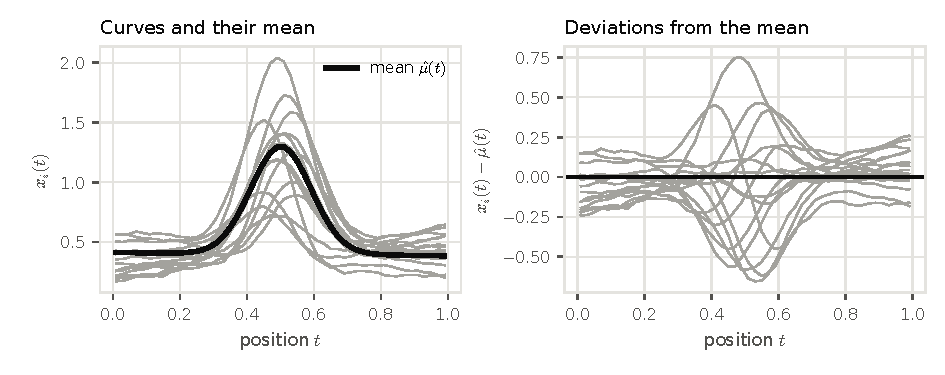
\includegraphics[width=\textwidth]{content/technical/figures/fpca_curves.pdf}
  \caption{Curves and their deviations from the mean. Left: 15 of 200 curves (grey) with their mean (black). Right: the same curves as deviations from the mean, which is what FPCA analyses. The curves are simulated and are not data from any cohort.}
  \label{fig:tech-fpca-curves}
\end{figure}

Whether the deviations at two positions tend to go together is described by the covariance function
\begin{equation}
  \Gamma(t, u) = \mathrm{cov}\{X(t), X(u)\},
  \label{eq:tech-fpca-cov}
\end{equation}
where $t, u \in [0, 1]$ are two positions on the domain.
At a single position, $\Gamma(t, t)$ is the variance of the curves there.
For two different positions, $\Gamma(t, u)$ is large when curves that lie above the mean at $t$ tend to lie above it at $u$ as well.
A feature that spreads over several neighboring positions, such as a peak whose height varies between curves, therefore shows up as a block of high covariance along the diagonal $t = u$ (Figure~\ref{fig:tech-fpca-cov}).

\begin{figure}[tbp]
  \centering
  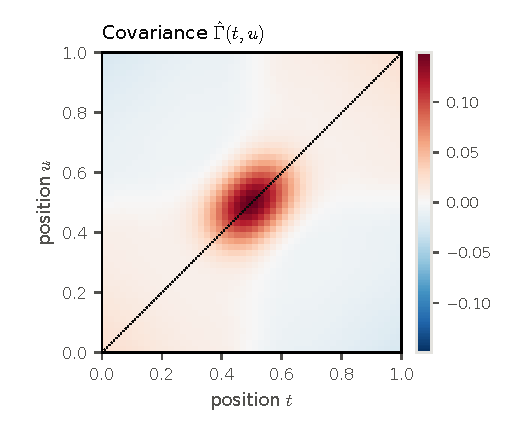
\includegraphics[width=0.55\textwidth]{content/technical/figures/fpca_covariance.pdf}
  \caption{Sample covariance function of the curves in Figure~\ref{fig:tech-fpca-curves}. Red marks pairs of positions at which the curves tend to deviate from the mean in the same direction, and the dotted line is the diagonal $t = u$, where the covariance is the variance. The block around $t = u = 0.5$ comes from the peak, whose height varies between curves at all of its positions together. The curves are simulated and are not data from any cohort.}
  \label{fig:tech-fpca-cov}
\end{figure}

The components are found by breaking this covariance down into shapes.
The first shape is the one along which the curves differ most, the second is the one along which they differ most among the shapes orthogonal to the first, and so on.
Formally, the shapes are the eigenfunctions $\phi_k$ of the covariance function, which is symmetric and non-negative definite, and each comes with an eigenvalue $\lambda_k$, so that
\begin{equation}
  \int_0^1 \Gamma(t, u)\, \phi_k(u)\, du = \lambda_k \phi_k(t),
  \qquad
  \int_0^1 \phi_k(t)\, \phi_{k'}(t)\, dt =
  \begin{cases} 1, & k = k', \\ 0, & k \neq k', \end{cases}
  \label{eq:tech-fpca-eigen}
\end{equation}
where $\lambda_1 \ge \lambda_2 \ge \dots \ge 0$ and the second condition makes the eigenfunctions orthonormal \cite{wang2016fda}.
Each eigenvalue is the variance of the curves along its eigenfunction, and the two together form a component.

\subsection{Scores and the Reconstruction of a Curve}
\label{sec:tech-fpca-scores}

A large positive score means that the curve deviates from the mean much like $\phi_k$, a large negative score means that it deviates the opposite way, and a score near zero means that the shape is nearly absent.
Formally, the score is the projection of the curve's deviation from the mean onto the eigenfunction,
\begin{equation}
  \xi_{ik} = \int_0^1 \{x_i(t) - \mu(t)\}\, \phi_k(t)\, dt ,
  \label{eq:tech-fpca-score}
\end{equation}
where $\xi_{ik}$ is the score of curve $i$ on component $k$.
The scores have mean zero and variance $\lambda_k$, and scores on different components are uncorrelated \cite{wang2016fda}.

Adding the shapes back to the mean, each weighted by its score, recovers the curve (Figure~\ref{fig:tech-fpca-rebuild}).
This is the Karhunen--Lo\`eve expansion, which in practice is truncated after $K$ terms \cite{wang2016fda},
\begin{equation}
  x_i(t) = \mu(t) + \sum_{k=1}^{\infty} \xi_{ik} \phi_k(t)
  \approx \mu(t) + \sum_{k=1}^{K} \xi_{ik} \phi_k(t),
  \label{eq:tech-fpca-kl}
\end{equation}
where the truncation replaces the curve by its first $K$ scores.
In Figure~\ref{fig:tech-fpca-rebuild}, the mean alone misses the height of the curve's peak, the first shape restores it, the second corrects the tilt along the domain, and the third adds almost nothing.

\begin{figure}[tbp]
  \centering
  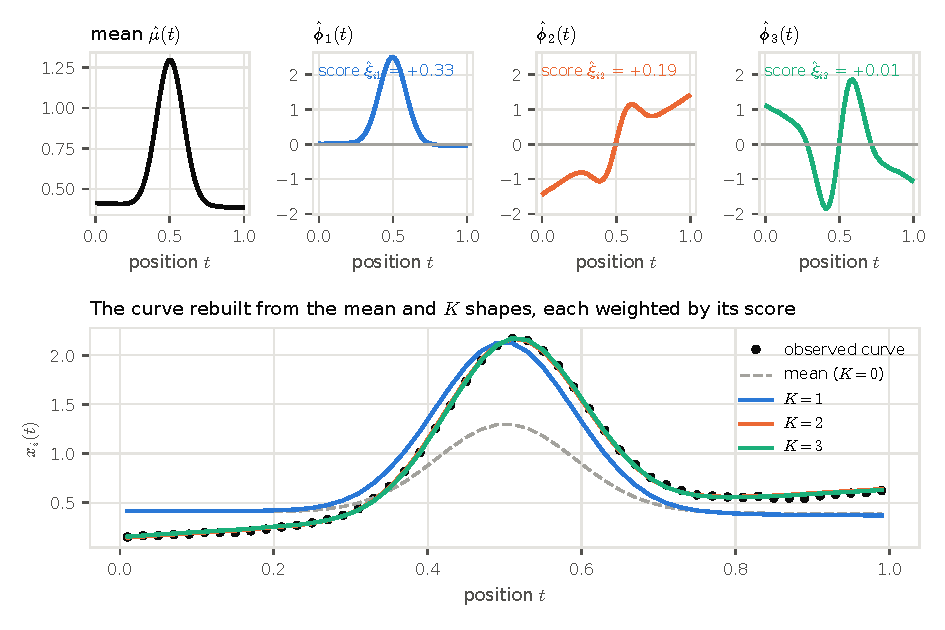
\includegraphics[width=\textwidth]{content/technical/figures/fpca_reconstruction.pdf}
  \caption{One curve rebuilt from the mean and the first three eigenfunctions. Top: the mean and the eigenfunctions, with the curve's score on each. Bottom: the observed curve (dots) and the curve rebuilt with $K = 0$ to $3$ components, each step adding one eigenfunction weighted by its score. The curves are simulated and are not data from any cohort.}
  \label{fig:tech-fpca-rebuild}
\end{figure}

The eigenfunctions thus serve as a basis for the curves, estimated from the curves themselves, and for a given $K$ no other set of $K$ basis functions approximates the curves with a smaller expected squared error \cite{wang2016fda}.
The price is that the components are specific to the sample, the domain and the preprocessing they were estimated from, so components from different samples describe different shapes.

\subsection{Reading the Components}
\label{sec:tech-fpca-reading}

An eigenfunction on its own has unit size and an arbitrary sign, so a component is shown instead by the mean together with the mean plus and minus a multiple of the eigenfunction, referred to as a mode of variation \cite{jones1992displaying, wang2016fda},
\begin{equation}
  \mu(t) \pm \alpha \sqrt{\lambda_k}\, \phi_k(t),
  \label{eq:tech-fpca-mode}
\end{equation}
where $\alpha$ usually ranges up to 2 \cite{wang2016fda}.
The curve for $+\alpha$ is the curve whose score on component $k$ lies $\alpha$ standard deviations above zero and whose other scores are all zero.
Plotted on either side of the mean, the two curves show what a high and a low score look like.
In Figure~\ref{fig:tech-fpca-modes}, a high score on the first component means a taller peak, and a high score on the second a curve that rises from the start to the end of the domain.
The name given to a component is a reading of this plot, not a tested property of the curves.

\begin{figure}[tbp]
  \centering
  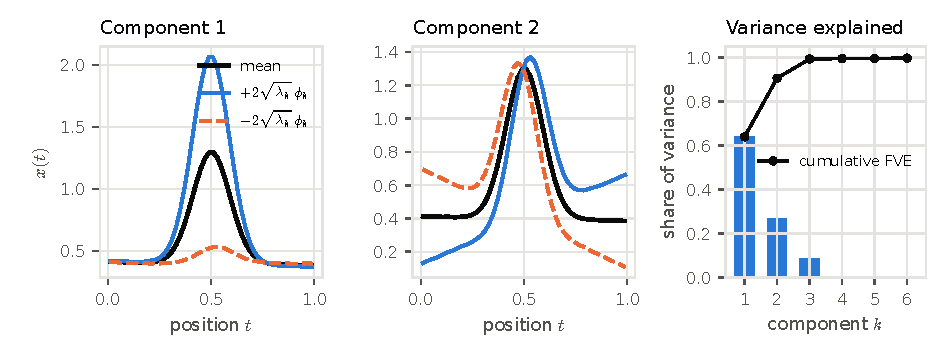
\includegraphics[width=\textwidth]{content/technical/figures/fpca_modes.pdf}
  \caption{Reading the components. Left and middle: the modes of variation of the first two components, with the mean (black) and $\mu(t) \pm 2\sqrt{\lambda_k}\,\phi_k(t)$ (colored). Right: the share of the variance per component (bars) and the cumulative fraction of variance explained (line), which levels off after three components. The curves are simulated and are not data from any cohort.}
  \label{fig:tech-fpca-modes}
\end{figure}

The arbitrary sign also matters when components are estimated more than once, since $-\phi_k$ solves Eq.~\eqref{eq:tech-fpca-eigen} whenever $\phi_k$ does, with the sign of every score $\xi_{ik}$ reversed.
A convention therefore fixes the sign, and components estimated again on bootstrap samples or cross-validation folds are aligned to it.
When the scores enter a cross-validated model, the mean and eigenfunctions are estimated within the training folds only, so the scores do not draw on the test curves.

\subsection{Choosing the Number of Components}
\label{sec:tech-fpca-k}

Each added component brings the rebuilt curves closer to the observed ones, but by less and less.
How much of the total variance the first $K$ components retain is measured by the fraction of variance explained,
\begin{equation}
  \mathrm{FVE}(K) = \frac{\sum_{k=1}^{K} \lambda_k}{\sum_{k \ge 1} \lambda_k},
  \label{eq:tech-fpca-fve}
\end{equation}
where the denominator equals $\int_0^1 \Gamma(t, t)\, dt$, the variance at each position summed over the domain.
Plotting the share of each component against $k$, referred to as a scree plot, shows where adding components stops paying (Figure~\ref{fig:tech-fpca-modes}, right).

Choosing $K$ is therefore a trade-off between keeping the main shapes and leaving out components that mostly describe noise.
A short expansion approximates the curves poorly, whereas each further component brings more estimation error, and no rule for the balance is established \cite{wang2016fda}.
The scree plot and thresholds on the fraction of variance explained are ad hoc rules carried over from ordinary principal component analysis \cite{wang2016fda}.
Of the information criteria, the Bayesian information criterion selects fewer components than the Akaike information criterion, and leave-one-curve-out cross-validation tends to select too many \cite{wang2016fda}.
Whatever the rule, it has to be fixed before the scores are related to an outcome.

The outcome plays no part in the components themselves, since FPCA builds them from the covariance of the curves alone \cite{wang2016fda}.
They are ranked by how much variance they describe, so a low-variance component can carry more information about the outcome than a leading one, and a leading one can carry none.
The covariance is a second moment, so a few outlying curves can shift its components \cite{wang2016fda}.

\subsection{Computation on a Grid}
\label{sec:tech-fpca-grid}

While FPCA is defined on continuous functions, curves are observed only at discrete points, so the integrals above cannot be evaluated directly.
When all curves are observed on one common grid of positions $t_g$, $g = 1, \dots, G$, each curve becomes a row of numbers, one per position.
The mean and covariance are then the sample mean and the sample covariance at the grid positions, and the eigenproblem becomes the eigendecomposition of a matrix \cite{wang2016fda}.
Curves observed at positions that differ between curves, or that are unevenly spaced, are first brought onto such a grid.

Let $\mathbf{D}$ be the $N \times G$ matrix with rows $\mathbf{d}_i$ and entries $d_{ig} = x_i(t_g) - \hat\mu(t_g)$, where $\hat\mu(t_g)$ is the sample mean at position $t_g$.
On an equally spaced grid with spacing $w = 1/G$, each integral is approximated by $w$ times the sum of its integrand over the grid positions, referred to as the rectangle rule.
Under this approximation, the eigenproblem~\eqref{eq:tech-fpca-eigen} reduces to that of the sample covariance matrix $N^{-1}\mathbf{D}^\top\mathbf{D}$, with unit-length eigenvectors $\mathbf{v}_k \in \mathbb{R}^G$ and eigenvalues $\tilde\lambda_k$.
The functional quantities then follow as
\begin{equation}
  \hat\lambda_k = w\, \tilde\lambda_k,
  \qquad
  \hat\phi_k(t_g) = w^{-1/2}\, v_{kg},
  \qquad
  \hat\xi_{ik} = w^{1/2}\, \mathbf{v}_k^\top \mathbf{d}_i ,
  \label{eq:tech-fpca-grid}
\end{equation}
where $v_{kg}$ is entry $g$ of $\mathbf{v}_k$ and $\hat\xi_{ik}$ is the score~\eqref{eq:tech-fpca-score} computed by the rectangle rule.
The factor $w^{-1/2}$ keeps the unit norm of Eq.~\eqref{eq:tech-fpca-eigen}, since the squared entries of a unit-length eigenvector sum to one, whereas the integral of $\hat\phi_k^2$ is approximated by $w$ times that sum.

FPCA on such a grid is therefore ordinary principal component analysis with the grid positions as variables, computed from the singular value decomposition of $\mathbf{D}$ \cite{warmenhoven2021pca}.
The factors in Eq.~\eqref{eq:tech-fpca-grid} only rescale the eigenvalues, eigenfunctions and scores.
They leave the shape of the eigenfunctions and the fraction of variance explained unchanged but set the units of the scores, so the scaling has to be stated for the scores to be interpretable.

\subsection{Registration: Amplitude and Phase}
\label{sec:tech-fpca-registration}

While the mean and covariance compare curves position by position, they assume that a feature lies at the same position $t$ on every curve.
Curves, however, differ both in how large a feature is, referred to as amplitude, and in where along the domain it lies, referred to as phase \cite{marron2015amplitude}.
If phase varies and is ignored, the mean taken position by position distorts the features and may resemble none of the curves (Figure~\ref{fig:tech-fpca-phase}) \cite{wang2016fda}.
Unaligned phase also inflates the variance and gives leading components that mix a shift of a feature with a change in its size \cite{marron2015amplitude}.

\begin{figure}[tbp]
  \centering
  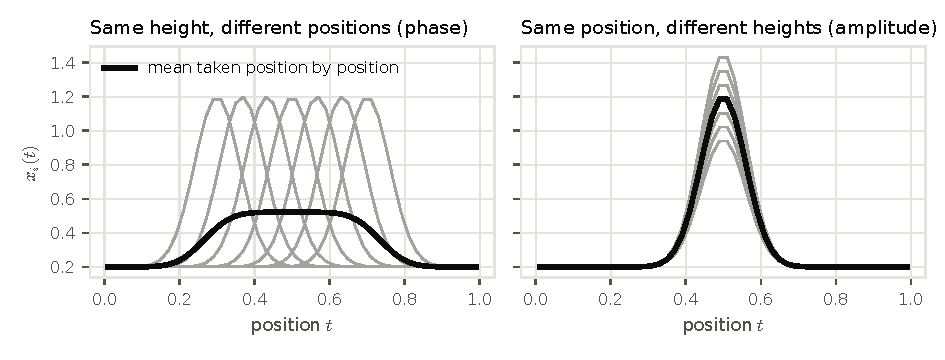
\includegraphics[width=\textwidth]{content/technical/figures/fpca_phase.pdf}
  \caption{Phase and amplitude. Left: seven curves with the same peak at different positions, whose mean taken position by position (black) is a low, wide plateau that resembles none of them. Right: seven curves with the peak at one position and different heights, whose mean keeps the shape of the peak. The curves are simulated and are not data from any cohort.}
  \label{fig:tech-fpca-phase}
\end{figure}

Registration addresses this by warping the domain of each curve with a strictly increasing function that keeps the two ends in place \cite{wang2016fda}.
The warp either moves landmarks, such as peaks, to their average position, or brings each curve close to a common template \cite{wang2016fda}.
Landmark registration is the reference method when clear features are present in every curve, but it fails when a landmark is missing or cannot be identified, which is common in noisy curves \cite{wang2016fda}.

When amplitude and phase vary together, the curves alone cannot tell them apart, so the assumptions built into the warp decide what counts as phase \cite{wang2016fda}.
Reading a component correctly therefore requires knowing which phase variation the registration has removed, if any.
Otherwise, a shift in where a feature lies may be read as a change in its size.


% Data chapter, 2 to 3 pages: the three complementary data sets. Section files in numeric order:
% 01 baseline CT volumes, 02 visual analysis (baseline and follow-up), 03 Medis centerlines and contours.
% The study cohort criteria are in sec:method-population, its counts in sec:results-cohort.
% Numbers from the 1,801-patient table (clean_baseline_count.py, clean_baseline_plaque_location.py on
% dtu-gpu-7) and CGPS_data/Medis_and_outcome/medis_match.md.
% Red notes need \usepackage{xcolor}. Remove before submission.
\providecommand{\clarify}[1]{\textcolor{red}{\textbf{Clarification needed:} #1}}

\chapter{Data}
\label{ch:data}

Three data sets from the Herlev--{\O}sterbro cohort were used in this thesis, each serving a complementary role.
The baseline coronary computed tomography angiography (CCTA) volumes were the input to the in-house tracer, whose centerlines and lumen were used to compute the geometric features; the visual analysis at baseline and follow-up defined the study cohort and the outcome; and the Medis centerlines and contours served as the reference for the tracer.
A summary of the three data sets is provided in Table~\ref{tab:data-overview}.

\begin{table}[htbp]
  \centering
  \caption{The three data sets, each linked to the others by the participant's study identifier.}
  \label{tab:data-overview}
  \small
  \begin{tabular}{p{0.16\linewidth}p{0.3\linewidth}p{0.12\linewidth}rp{0.18\linewidth}}
    \toprule
    Data set & Content & Visit & Scans & Used for \\
    \midrule
    CT volumes & non-contrast and CCTA volumes & baseline & [n] & in-house tracer and geometric features \\
    Visual analysis and patient characteristics & stenosis grade and plaque type per segment; SIS and SSS & baseline and follow-up & 1,801 & cohort and outcome \\
    Medis centerlines and contours & centerline trees labelled by segment; lumen and plaque contours of the main vessels with plaque & baseline & 600 / [n] & reference for tracer centerlines and lumen \\
    \bottomrule
  \end{tabular}
\end{table}

% The data set as delivered (1,801-patient table, Kit 2026-10-28) and the baseline CT volumes, input
% to the in-house tracer. Only the data set is described here; the restriction to the study cohort
% is in methodology/02_population_outcome.tex (sec:method-population).
% Follow-up interval: section 1 of the cgps_stats.py report on the 1,801-patient table.
\section{Study Population and CT Volumes}
\label{sec:data-cohort}

The Copenhagen General Population Study, referred to in this thesis as Herlev--{\O}sterbro, is a prospective cohort study of adults from the Greater Copenhagen area, randomly selected from the Danish Civil Registration System.
Within this cohort, a subset of the participants underwent CCTA, and those scanned again at a follow-up visit form the basis of this thesis.
The data set comprises 1,801 participants, scanned a median of [..] years apart (interquartile range [..]--[..] years).
The study cohort drawn from it is defined in Section~\ref{sec:method-population}.

At each visit, a non-contrast, electrocardiogram (ECG)-gated scan was acquired for coronary artery calcium scoring, followed by contrast injection and an ECG-gated CCTA.
Only the baseline CCTA volumes were analysed in this thesis, serving as input to the in-house tracer (Section~\ref{sec:method-tracer}) and providing the centerlines and lumen from which the geometric features were computed.
The follow-up scans contributed through their visual analysis (Section~\ref{sec:data-plaque-location}).
\clarify{ number of baseline volumes received; scanner, tube voltage, contrast and reconstruction (voxel size, kernel).}

% Visual analysis at baseline and follow-up: what was read. The cohort criteria and outcome are in
% methodology/02_population_outcome.tex (sec:method-population); where incident plaque developed is in
% results/00_cohort.tex (sec:results-cohort), moved there 2026-10-31.
\section{Visual Analysis and Patient Characteristics}
\label{sec:data-plaque-location}

Every baseline and follow-up CCTA was analysed visually.
\clarify{how and by whom the visual analysis was made.}
For each of the 17 coronary segments, the reader recorded the stenosis grade (none, minimal, mild, moderate, severe, or occlusion), the plaque type (calcified, mostly calcified, mostly non-calcified, or non-calcified), high-risk plaque features, and evaluability.
The reads were summarised per participant in the segment involvement score (SIS) and the segment stenosis score (SSS), counting the segments with plaque and summing the stenosis grades, respectively.
In the delivered baseline table, segments without a grade are filled with none, and whether a scan was read is recorded in a separate flag; all 1,801 baseline scans were read.

All SCORE2 risk factors \cite{score2_2021} were also recorded at both visits: age, sex, current smoking, systolic blood pressure, and total and high-density lipoprotein (HDL) cholesterol, from which non-HDL cholesterol is derived.

% Medis centerlines and contours as delivered: what they are and whom they cover. How they are used
% (comparison with the tracer, collapsing segments to arteries, contour matching, coordinates, and
% that the comparison lies outside the plaque-free cohort) is in methodology/01b_medis_reference.tex
% (sec:method-medis); do not repeat it here. Rewritten 2026-11-01.
% Counts from the HØ_10Y Medis delivery (CGPS_data/CLAUDE.md) and:
%   CGPS_data/Medis_and_outcome/medis_match.md (2026-10-29): 600 trees, all matched in BL and FU;
%     599 plaque at BL, <5 plaque-free (suppressed; 600 - 599 makes it recoverable, see chat 2026-10-31).
%   CGPS_data/Medis_and_outcome/medis_missing_plaque.md (2026-10-31): 724 with plaque at BL; 599 of
%     them have a tree, 120 of the other 125 have _medis_finished = 1.
\section{Medis Centerlines and Contours}
\label{sec:data-medis}

Two further data sets were made in Medis from baseline scans and delivered together with a log of their extraction.
The first holds centerline trees of the coronary arteries for 600 scans, labelled by coronary segment.
The second holds 3,049 contour segments of the lumen and the outer vessel wall, made only for segments with plaque.
\clarify{how the trees and contours were made (traced by Medis, corrected by a reader, or both) and on what criterion the scans were selected; how many scans lie behind the 3,049 contour segments and how many of them also have a tree; in how many trees the LAD, LCx and RCA are complete.}

Every tree was linked by its study identifier to a participant in both the baseline and the follow-up table.
Of these 600 participants, 599 had plaque at baseline and fewer than five were plaque-free.
The trees cover 599 of the 724 participants with plaque at baseline (82.7\%).
For 120 of the remaining 125, the baseline table records the Medis plaque analysis as finished, which suggests that their trees are missing from the delivery rather than never made.
Their plaque location, number of segments with plaque and worst stenosis grade were similar to those of the participants with a tree.
\clarify{ask Kit whether a tree was made for every scan with plaque (so the 125 are lost in the delivery) or only for some, and on what criterion. The finished flag is filled only for segments the visual analysis graded as plaque, so it is not an independent check.}



% Chapter opener (rewritten 2026-10-31, Aida-style single paragraph; refactored 2026-11-06 to nine
% stages, one per section, in \input order). Moved from thesis/methodology/00_chapter_intro.tex
% on 2026-11-07. \input order is in content/methods.tex:
%   01a-02b   full text
%   03-07     notes only, to be written
% Overview figure still to make (style guide: an overview figure opens the methods).
\providecommand{\clarify}[1]{\textcolor{red}{\textbf{Clarification needed:} #1}}
\chapter{Methodology}
\label{ch:methodology}

The methodology followed in this thesis is summarized in Figure~\ref{fig:method-overview} and consists of nine main stages:
(1) extraction of the coronary centerlines and lumen contours from all baseline scans with an in-house tracer;
(2) comparison of the extracted centerlines and lumen with Medis as a reference, as no ground truth was available;
(3) selection of the plaque-free baseline cohort and definition of the outcome from the visual analysis;
(4) division of the traced arteries into the segments of the visual analysis;
(5) the prediction model and its cross-validation;
(6) the number of parameters the cohort can support and the choice of geometric features within it;
(7) definition of the geometric features;
(8) assessment of their measurement properties, against synthetic shapes and known groups, and of the variance explained by known risk factors;
and (9) a secondary, descriptive analysis of the shape of the curvature profile.

\clarify{overview figure of the nine stages (label fig:method-overview).}

% TotalSegmentator -> start points -> in-house tracer (Kit Mills Bransby). Not the author's
% contribution, so only outputs and how it was run on CGPS; the author's check is sec:method-medis.
% Each red [Qn] blank is answered by Qn in the list below; fill the blanks, then delete the list.
% Red notes need \usepackage{xcolor}. Remove before submission.

\newpage

\providecommand{\clarify}[1]{\textcolor{red}{\textbf{Clarification needed:} #1}}
\providecommand{\ask}[1]{\textcolor{red}{[#1]}}
\section{Coronary Centerline and Lumen Extraction}
\label{sec:method-tracer}

To extract the coronary centerlines and lumen from the baseline CCTA volumes, an in-house tracer was applied to all scans of the Herlev--{\O}sterbro cohort (Section~\ref{sec:data-cohort}). The in-house tracer was developed and run by Kit Mills Bransby. The method is described here so that the full pipeline is shown. 


\clarify{Questions for Kit:
\begin{enumerate}
  \item Can you give a brief description of the tracer. Should we call it in-house tracer or do you have a better name for it?
\end{enumerate}}

% Comparison of the in-house tracer (sec:method-tracer) with the Medis reference (sec:data-medis).
% Shortened 2026-11-01 from the 2026-10-31 version (source: reports/Centerline and lumen contour
% comparison.md); the general definitions (correspondence, OV/OT/AI, limits of agreement) are in
% technical_background/07_agreement.tex (sec:tech-agreement). Limitations (single reader, plaque-only
% reference, shared imaging errors) go in the Discussion.
% Every threshold marked [x] is a design choice without a published value; fix it before the
% comparison is run and before any outcome analysis, never tune it on the result.
% Red clarification notes; needs \usepackage{xcolor} in the preamble. Remove before submission.
\providecommand{\clarify}[1]{\textcolor{red}{\textbf{Clarification needed:} #1}}
\section{Medis Reference as validation for the in house tracer output}
\label{sec:method-medis}

No ground truth exists for the Herlev--{\O}sterbro scans, so the quality of the centerlines and lumen contours from the in-house tracer (Section~\ref{sec:method-tracer}) cannot be measured directly.
Instead, they were compared to the Medis centerlines and the semi-manually annotated Medis contours of the same baseline scans (Section~\ref{sec:data-medis}), which gives an indirect estimate.
Medis: \clarify{how were they exactly produced and handled (semi corrected?} 
Medis data exist only for participants with plaque at baseline, so the comparison was made outside the plaque-free study cohort.

The tracer and Medis label their centerlines at different levels.
Medis labels each point of its centerlines with a segment, such as the \textbf{proximal} LAD, whereas the tracer labels only the artery.
To measure the tracing error rather than a difference in where the tracer and Medis place the segment boundaries, the proximal, mid and distal Medis segments of each artery were collapsed into one full artery.
This thesis uses only the LAD, LCx and RCA (Section~\ref{sec:method-population-arteries}), so the comparison was limited to these three arteries.

\subsection{Agreement Between the Tracer and Medis}
\label{sec:method-medis-agreement}
The centerlines and contours enter the prediction model only through the geometric features computed from them (Section~\ref{sec:method-features}).                                                                           
Therefore the agreement was measured on the features and not the points themselves.
First the tracer centerlines and contours were mapped into the coordinates of Medis, and each tracer artery was paired with the Medis artery of the same participant and label.
\clarify{in which coordinates are the Medis points stored: LPS millimeters, RAS millimeters or voxel indices? And in which coordinates does the tracer store its points?}

Centerline features were computed on the full artery without any adjustments, whereas the lumen contour features were computed only over the part of the artery covered by the Medis lumen contours.
To achieve this, the tracer centerline was cut where the first and the last Medis lumen contour lie \cite{schaap2009cat08}, which cut its lumen contours to the same stretch.


% Study cohort and outcome, written for a first-time reader (rewritten 2026-11-02; arteries and
% segments moved to 02b_segment_split.tex). Definitions only: the counts (flowchart, incident plaque per artery)
% are in results/00_cohort.tex (sec:results-cohort), what the visual analysis recorded is in
% data/02_visual_analysis.tex, and the overlap with the Medis trees in data/03_medis_reference.tex.
% Does not repeat data/01-03: cohort size, segment grading, SIS/SSS, Medis coverage.
% The choice of arteries (sec:method-population-arteries), why the analysis is per segment and the
% division into segments (sec:method-split) and its check (sec:method-split-validation) are in
% 02b_segment_split.tex; the landmark table is in appendix/B_segment_split_details.tex.
% Does not repeat clinical_background_v2 (sec:wss, sec:tree).
% Still open: follow-up time enters the model as log(years); missing baseline geometry (open
% decision 9); partly graded FU arteries.
% [..] and \clarify{} mark information that is not yet available; nothing there is to be guessed.
\providecommand{\clarify}[1]{\textcolor{red}{\textbf{Clarification needed:} #1}}
\section{Study Cohort and Outcome}
\label{sec:method-population}

The study cohort comprised the Herlev--{\O}sterbro participants without coronary plaque at baseline, defined by a segment involvement score (SIS) of zero (Section~\ref{sec:data-plaque-location}).
Participants with insufficient image quality ([criterion]) were also excluded, and the resulting cohort is described in Section~\ref{sec:results-cohort}.
The primary outcome was incident coronary plaque, defined at the segment level as a stenosis grade of minimal or worse and at the participant level as plaque in at least one of the analysed segments (Section~\ref{sec:method-population-arteries}).
In a sensitivity analysis, the outcome was restricted to plaque with mild or worse stenosis.
% Counts (65 RCAs, 5 LCxs, <5 LADs) belong in results/00_cohort.tex, not yet there.

\clarify{The outcome could still change!!!}

% Coronary segments: the choice of arteries, their division into proximal, mid and distal
% segments, and a check of the division. Short main text (user, 2026-11-02): the exact division,
% thresholds and the landmark table are in appendix/B_segment_split_details.tex (sec:app-split).
% Placed after 02_population_outcome. Humanised 2026-11-02 in the style of clinical_background_v2.
% Does not repeat: tracer labels only the artery, Medis by segment (01b, sec:method-medis-arteries);
% what the visual analysis and the Medis trees and contours are (data/02, data/03).
% Division: CGPS_data/split_trunks.py (landmark_cuts). Check: CGPS_data/thesis_final/split_check.py
% --trees tracer, section 2 (contours by location vs the visual BL grade: a contour whose majority
% segment is not graded plaque = miss); reference run --trees medis.
% Red clarification notes; needs \usepackage{xcolor} in the preamble. Remove before submission.
% 2026-11-09: "further down, in the LAD and LCx" -> "at the start of the LAD and LCx, just beyond the
%   bifurcation", to agree with sec:method-features (angle and ratios enter only the proximal LAD
%   and LCx). CHECK: the review now ties the LM angle to low WSS at the bifurcation (Garcha,
%   simulations) and plaque to bifurcation outer walls (van der Giessen), but no study in it relates
%   the LM angle itself to disease; the study behind the original sentence (cui2017bifurcation?) was
%   cut from the review. Soften to "low WSS" or restore the source.
\providecommand{\clarify}[1]{\textcolor{red}{\textbf{Clarification needed:} #1}}
\section{Analysed Arteries and Segments}

\subsection{Choice of Arteries}
\label{sec:method-population-arteries}

The analysis covered the three main coronary arteries, the left anterior descending (LAD), the left circumflex (LCx) and the right coronary artery (RCA), both for the outcome and for the geometric features.
These arteries are present in every heart, whereas the number and size of the side branches vary between individuals and with dominance (Section~\ref{sec:dominance}).
Their larger diameter also makes the measurements less sensitive to error: with a voxel size of [..]\,mm, an error of one voxel at the lumen boundary corresponds to about [..]\% of the diameter of a main artery \cite{dodge1992diameter}, compared with [..]\% for a side branch \clarify{voxel size; side-branch diameter and its citation}.
The left main (LM) was also left out.
None of the studies in the literature review related LM geometry to plaque in the LM itself; the angle of the LM bifurcation was instead related to disease at the start of the LAD and LCx, just beyond the bifurcation (Chapter~\ref{ch:literature}).
A participant who developed plaque only in the LM or in a side branch was therefore counted as without the outcome.
This applied to a small proportion of participants (Section~\ref{sec:results-cohort}), and the implications of this misclassification are addressed in Section~[..] \clarify{discussion section on this misclassification, not yet written}.                                                                           

\subsection{Division into Segments}
\label{sec:method-split}

Geometry is theorised to influence plaque formation through low wall shear stress, which is a local force. 
A feature averaged over a whole artery would risk blurring these local differences, so the features were computed at the same fine resolution as the outcome.
Each of the three arteries was therefore divided into a proximal, a mid and a distal segment, giving nine segments per participant (Figure~\ref{fig:method-segments}).

The visual analysis does not record where one segment ends and the next begins, so a landmark division method was developed and used in this thesis to place the boundaries.
Where no such branch was available, the boundary was placed at a fixed fraction of the distance along the artery.
The full division is given in Appendix~\ref{sec:app-split}.

% Figure from segment_selection_schematic.py (made-up tree, no patient data).

\subsection{Validation of the Division}
\label{sec:method-split-validation}

To give an indication of the reliability of the division, the Medis lumen contours were projected onto the nearest points of the divided tracer artery, and the segment holding the largest part of each contour was looked up in the visual analysis.
If that segment was not graded with plaque at baseline, a miss was recorded.
Only the position of the contour was used, not the segment name Medis gave it, so the check does not depend on how Medis divided the artery.
The miss rate is reported in Section~\ref{sec:results-cohort}.
A slightly displaced boundary moves only a few points at either end of a segment, so features computed per segment were preferred, despite this uncertainty, to features averaged over the whole artery.

% NOTES ONLY, to be written. Trimmed 2026-11-07 from thesis/methodology/03_prediction_model.tex
% (full draft in git, commit e4eb857).
% Design: root CLAUDE.md "Decided". Settings come from CGPS_data/progression_who_pooled.py, which is
% not in CGPS_data/thesis_final/ and still runs on the Medis trees with a progression outcome; the
% text must follow the clean-cohort version once it exists there.
%
% The section should contain:
% - One segment-level complementary log-log GLMM over the nine segments, random intercept per
%   participant (sec:tech-segment-glmm). One row per segment, outcome incident coronary plaque in
%   that segment (sec:method-population).
% - Segment risks pooled into one person risk of plaque in any of the nine segments
%   (sec:tech-aggregation); the person risk is what is evaluated.
% - Fit: maximum likelihood, Gauss-Hermite quadrature over the random intercept. Open: node count
%   (30 in the script, checked by a refit with doubled nodes).
% - Open (added 2026-11-13): random-effects structure. The person intercept makes every pair of
%   segments equally correlated (pLAD-mLAD as pLAD-dRCA); segments on one artery likely share more
%   (inflow, plaque across segment boundaries). Effect: LR test rejects too often (already in
%   sec:tech-glmm-likelihood), and the person risk is overstated if plaques cluster within an artery.
%   Options: (a) add a person x artery intercept (LAD, LCx, RCA), nested in person; about three
%   segments per artery and few events, so its variance may not be identifiable; (b) check residual
%   correlation for same-artery vs different-artery pairs after the fit; (c) if (a) fails, keep the
%   person intercept and state it as a limitation in the Discussion. Intervals from person-level
%   resampling (CV, bootstrap) hold whatever the dependence; only the LR test leans on the intercept.
%   Not a case for GEE: an exchangeable working correlation makes the same assumption, and GEE gives
%   no joint distribution for the person risk. Theory: sec:tech-nested.
% - Base model: segment position (pLAD reference), log segment length, dominance, log follow-up
%   time, SCORE2 risk factors. Open: follow-up as term or offset; recalibrated SCORE2
%   (sec:tech-recalibration) vs refitted SCORE2 factors, compared in this pooled model.
% - Extended model: base + geometry block (four features, sec:method-selection: curvature, taper,
%   bifurcation angle, daughter asymmetry ln(D_LCx/D_LAD); each its own linear term; Finet's ratio
%   dropped 2026-11-13, see 05c header),
%   standardised within segment type on the training participants. Open: which segment rows carry the
%   left main angle and asymmetry (script: pLAD and pLCx rows only).
% - Secondary (decided 2026-11-11): angle x asymmetry, one prespecified term, estimated and reported,
%   outside the LR test of the block (a product needs its main effects; support is one simulation
%   study on synthetic trees, garcha2025sensitivity). sec:method-ratio points here.
% - One prespecified LR test of the geometry block (eq:tech-lr), both models on all participants.
%   Delta C, calibration slope and intercept, Brier score and log loss estimated with intervals,
%   never tested (sec:tech-added-value).
% - Where: read descriptively from the same model (feature hazard ratios, segment intercepts,
%   within-participant C, secondary curvature/taper x artery test). No separate where model.
% - Subsection Cross-Validation (sec:method-cv): folds by participant, all nine segments in one
%   fold, stratified on developing plaque. Same folds for base and extended model; standardisation,
%   coefficients and random-intercept variance estimated on training participants of each fold.
%   Report mean over repeats with 2.5th/97.5th percentiles and the paired difference. Open: folds and
%   repeats (10 x 50 in the script); percentiles show split variation, not sampling uncertainty,
%   so state whether difference intervals come from a bootstrap of the whole procedure.
\section{Risk Model and Evaluation}
\label{sec:method-models}

\todonote{To be written: the pooled cloglog GLMM, its base and extended model, the LR test of the geometry block and the estimated performance measures. See the notes in the source.}

\subsection{Cross-Validation}
\label{sec:method-cv}

\todonote{To be written: person-level folds, stratified on the outcome, and how the measures are summarised.}

% NOTES ONLY, to be written. Trimmed 2026-11-07 from thesis/methodology/04_model_size.tex
% (full draft in git, commit e4eb857).
% Outcome-blind: the budget uses only participants and events, never geometry; the selection uses
% only the literature and measurement properties, never association with plaque.
% Numbers: CGPS_data/who_where_readiness.py still uses 10/20 events-per-parameter rules; switch it to
% the Riley criteria (pmsampsize) first. Plan: ~/Desktop/Speciale/CGPS_statistics-/CLAUDE.md, open
% decision 11 (about 15 to 20 parameters at C = 0.70).
%
% The section should contain:
% - Opening: model size and features fixed before baseline geometry is linked to follow-up plaque,
%   so the LR test tests geometry, not earlier choices. First the budget, then the selection.
% - Subsection Parameter Budget (sec:method-size-budget): Riley criteria (sec:tech-sample-size),
%   shrinkage S = 0.9, anticipated C = 0.70 (source needed, e.g. PARADIGM clinical-only 0.68), also
%   0.65 and 0.75. Participants, events and P_max to fill in. Open: the criteria are for a binary
%   person-level outcome; state that n and events are counted per participant.
%   Degrees-of-freedom counting (linear 1, spline k-1, factor m-1, interaction >= 1), base first,
%   geometry gets the rest, all geometric terms linear, part of the budget left unused on purpose.
%   Table tab:method-size-budget (participants, events, P_max, base df, geometry 5, used, unused).
%   Open: SCORE2 factor coding; whether an absent-left-main indicator joins the geometric block.
% - Subsection Selection of Geometric Features (sec:method-selection): candidates are geometry the
%   literature (ch:literature) ties to WSS or plaque location and the tracer output allows. One
%   primary definition each, others to sensitivity (sec:method-validity-definitions). Candidates set
%   aside for weaker literature support (tortuosity index, bend counts, side-branch bifurcations),
%   [2026-11-07 CHECK: the Literature Review now supports tortuosity index (sec:lit-wss Kashyap,
%   sec:lit-measure), bend counts (sec:lit-measure Li) and LM-daughter angles (sec:lit-wss Cui, moved 2026-11-07);
%   "side-branch bifurcations" has no source in the review: find one or drop it.]
%   measurement error on CCTA (torsion, eccentricity, local expansion, pointwise profiles, lumen
%   volume to myocardial mass) or overlap with a retained feature (curvature x
%   calibre, upstream curvature, distance from ostium, side-branch count). Prose only, no table.
%   Four features remain: segment curvature and taper, LM angle, daughter asymmetry (2026-11-13:
%   Finet's ratio dropped, no supporting literature and the only feature needing the LM diameter;
%   see 05c header). Coverage [..]% of the cohort; the asymmetry is available whenever the angle is.
%   Budget: geometry block 4 df, plus 1 for the secondary angle x
%   asymmetry term outside the LR test. No ranking, screening, stepwise or penalised
%   selection; the rest go to secondary analyses.
% HONESTY CHECK: say the four were prioritised on these criteria, NOT that a longer list was ranked.
% 2026-11-09: the shared reason for the five (shape disturbs flow and lowers WSS, one sentence per kind
%   of feature, tied to low WSS in sec:lit-wss) is now stated once in 05_features.tex
%   (sec:method-features). sec:method-selection should only say why these four were kept over the
%   other candidates, and point to sec:method-features for the haemodynamic rationale.
\section{Parameter Budget and Feature Selection}
\label{sec:method-size}

\todonote{To be written: how many parameters the cohort supports and which geometric features fill them. See the notes in the source.}

\subsection{Parameter Budget}
\label{sec:method-size-budget}

\todonote{To be written: Riley criteria, the anticipated C-statistic and the allocation table.}

\subsection{Selection of Geometric Features}
\label{sec:method-selection}

\todonote{To be written: the candidates, why each set-aside one was set aside, and the four retained features.}

% NOTES ONLY, to be written. Trimmed 2026-11-07 from thesis/methodology/05_features.tex and
% 05a-05d (full drafts in git, commit e4eb857). Figures still in thesis/methodology/:
% features_overview_schematic.{py,pdf} and turning_feature_schematic.{py,pdf}.
% CHECK: CGPS_data/thesis_final/ holds only turning_feature.py and split_check.py; taper, angle and
% ratios have no final script yet, so their text cannot be written to the code yet.
%
% Umbrella section should contain:
% - Features drawn from studies relating geometry to low WSS or plaque location (ch:literature,
%   sec:method-selection), some adapted (curvature on 3D centerlines over a fixed chord).
% - Read from the arteries of sec:method-split, points in mm with an artery label, traversed from
%   the ostium. Open: in split_trunks.py the LAD and LCx paths start at the LM bifurcation, not at
%   the ostium; only the RCA starts at the ostium.
% - Curvature and taper per segment; angle and ratios once per participant at the LM bifurcation.
%   Open: the split points carry no lumen radius, and the tracer gives a contour per step, not a mask.
% - Table tab:method-features (feature, measured on, input, section) and the overview figure
%   fig:method-features.
% - Shared rules: unit of measurement; missing values (TODO).
\section{Geometric Features}
\label{sec:method-features}

\todonote{To be written: where the features come from, what they are read from, and the overview table and figure.}

% NOTES ONLY, to be written. Trimmed 2026-11-07 from thesis/methodology/05a_curvature.tex
% (full draft in git, commit e4eb857). Implementation: CGPS_data/thesis_final/turning_feature.py
% (mean_turning, segment_turning) on each artery from split_trunks.py; figure from
% turning_feature_schematic.py.
%
% The subsection should contain:
% - Curvature as mean turning angle per mm, a form of average curvature, the tortuosity measure most
%   closely, although weakly, related to low WSS (kashyap2022tortuosity; simulation study, keep
%   "although weakly").
% - Turning angle at each point between two 5 mm chords, chord ends by linear interpolation;
%   atan2 form (eq:method-turn), unsigned in [0, pi].
% - Noise: a positional error sigma gives spurious turning that falls with the square of the chord
%   length; 5 mm chord as in vanzandwijk2019curvature. No further smoothing; no values within 5 mm of
%   either artery end. TODO: confirm with Kit that the tracer centerlines arrive smoothed.
% - Profile kappa = theta / l in rad/mm (eq:method-profile, referred to by curvature_fpca), computed
%   on the whole artery and then divided at the segment boundaries.
% - Segment value T_s = arc-length mean of the profile (eq:method-tl), trapezoid rule; fewer than two
%   profile points -> missing.
% - Difference from Tello Ayala et al. (2D, consecutive points): 3D, fixed chord, normalised by
%   length, so independent of point spacing.
% - Figure fig:method-turning.
\subsection{Turning-angle curvature}
\label{sec:method-curvature}

\todonote{To be written: turning angle over 5\,mm chords, the curvature profile and its arc-length mean per segment.}

% Methods, subsection of sec:method-features: the bifurcation angle only. Which segments it enters
% (proximal LAD and LCx) and why belong to 05_features.tex, how it enters the model to
% sec:method-models.
% Implementation (since 2026-11-10): CGPS_data/thesis_final/bifurcation_angle.py (point_at_depth,
% angle_between, lm_angle, tree_angle; DEPTHS = 5 to 10 mm in 0.5 mm steps) on the LAD and LCx
% arteries of split_trunks.split. Replaces who_where_readiness.lm_bifurcation_angle (Medis labels,
% centroid of points 2 to 8 mm, one bifurcation point per daughter; no published source).
% Source: Medrano-Gracia et al. 2016 (medranogracia2016atlas), read in full 2026-11-10: "A bifurcation
%   point was automatically calculated from the centrelines at the point where the centrelines split";
%   measurements "at a range of depths from this bifurcation point in 0.5 mm steps, following the
%   centrelines" (arc length); angle B "the angle of the bifurcation between the distal main vessel
%   and the side branch" (for the LM: LAD to LCx); "Computationally, these angles have to be defined
%   with linear approximations of the centrelines"; reported "as the average in the 5-10 mm depth
%   interval"; "averaging angles in the 5-10 mm interval ensures a more robust measurement than a
%   single point" (word "robust" is theirs, not used here); the angle "slowly decreases as the
%   measurement is taken further from the bifurcation point". Their values: 78.9 +- 23.1 deg (N = 300),
%   89 deg with and 75 deg without an intermediate artery.
% CHECK: how the "linear approximations" were fitted is not stated. The code uses the line from the
%   bifurcation point to the centerline point at each depth; keep "follows", never "replicates".
% CHECK: the bifurcation point is the first point shared by the tracer LAD and LCx
%   (split_trunks.split starts both there when their paths share a node; otherwise the paths start after
%   a labelled LM, the points differ and the angle is missing). How often this happens in the tracer
%   trees is unknown until they are run.
% OPEN: ramus intermedius. The tracer labels only the artery, so a ramus is not separated; the atlas
%   found the angle 14 deg wider with one. Handling belongs to sec:method-validity-definitions.
% CAREFUL: progression_who_pooled.py still takes the angle from the old Medis function, so the model
%   and this text disagree until that script calls tree_angle.
% Not used: angle A or C, the inflow angle (their own definitions, not in the five features), 2D
%   projection (EBC: 3D is needed). Not stated in the text (counterfactual rule).
% 2026-11-10 (user: Aida methodology guide over sec:method-angle; no "The feature chosen", no
%   First/Finally). Facts, cite, label and eq:method-angle unchanged. Changed: opener chains to the
%   division into segments and names the input (guide 4.1); equation chain with a where sentence naming
%   every symbol and one sentence on what theta tells (9.1); the mean over depths is now an equation,
%   eq:method-angle-mean (9.1); the depth interval as concede-and-defend with its cost named (5); step
%   markers removed, each step opens with what is measured. Cut: "since the tracer labels only the
%   artery ..." (a reason about the tracer's design that was not checked against the labels).
\subsection{Bifurcation Angle}
\label{sec:method-angle}

Note: Research if this is better to have two angles going into the model proximal main vessel and the side branch, and angle the angle between the proximal and distal main vessel. Also research if the inflow angle is important and should be included.

 
The bifurcation point $O$ was taken as the first centerline point shared by the LAD and the LCx, where their arc length starts.
At the arc length $d$ from $O$, the points $L(d)$ on the LAD and $C(d)$ on the LCx were found, and the angle between the lines from $O$ to these points was computed as
\begin{equation}
  \theta(d) = \operatorname{atan2}\!\left( \lVert (L(d) - O) \times (C(d) - O) \rVert ,\; (L(d) - O) \cdot (C(d) - O) \right) ,
  \label{eq:method-angle}
\end{equation}
where $\times$ and $\cdot$ denote the cross product and the dot product of two vectors, $\lVert \cdot \rVert$ the length of a vector, and $\operatorname{atan2}$ the angle that has this cross-product length and this dot product.
$\theta(d)$ lies between 0 and 180 degrees, and a wider angle means that the two arteries leave the bifurcation further apart.

The bifurcation angle $\bar\theta$ was the mean over the depths from 5 to 10\,mm in steps of 0.5\,mm:
\begin{equation}
  \bar\theta = \frac{1}{11} \sum_{d \in \{5,\,5.5,\,\ldots,\,10\}} \theta(d) ,
  \label{eq:method-angle-mean}
\end{equation}
where the eleven depths are in mm along the arteries from $O$.
Although the angle depends on the depth at which it is measured, this interval follows Medrano-Gracia et al., who used it because the angle decreases slowly with depth, and averaging over it keeps $\bar\theta$ from resting on one depth.
The cost is that bends in the first 10\,mm of the arteries enter the angle.
$\bar\theta$ was recorded as missing for participants whose LAD and LCx share no first point or whose LAD or LCx is shorter than 10\,mm.

% Methods, subsection of sec:method-features: the two diameter-ratio features only. Why the bifurcation
% is represented at all belongs to sec:method-features and sec:lit-wss; which segment rows they enter
% (proximal LAD and LCx) to 05_features.tex and sec:method-models.
% 2026-11-11: written from daugther_ration_plan.md (same folder). Replaces the notes trimmed 2026-11-07
% (full draft in git, commit e4eb857).
% Decision (with the user, 2026-11-11): two features, still 2 parameters: daughter asymmetry
%   ln(D_LCx / D_LAD) and Finet's ratio D_LM / (D_LAD + D_LCx). Angle and the two ratios keep their own
%   linear terms in the tested geometry block (5 parameters); angle x asymmetry is one prespecified
%   secondary term, estimated, outside the LR test (one simulation study on synthetic trees, and a
%   product needs its main effects). Owned by sec:method-models.
% Rejected, not stated in the text (counterfactual rule): the LM->LAD and LM->LCx ratios planned
%   before 2026-11-11. Both divide by the LM diameter, the least reliable of the three (LM length
%   10.5 +- 5.3 mm in Medrano-Gracia 2016, so the stretch clear of the ostium and of the confluence is
%   short or absent); its error enters both and correlates them, and both go missing together. The
%   review supports the LAD-LCx width difference (Garcha 2025) and discusses Finet's ratio (Zhang 2024,
%   null); neither used LM->daughter ratios.
% Murray's exponent 3, the pooled 2.39 (taylor2024murray) and 7/3 (huo2012scaling) are no longer
%   needed here; the fact-ownership line for them in the content map (Thesis_coronary/CLAUDE.md) lapses.
% Implementation: CGPS_data/thesis_final/daughter_ratio.py (contour_area, contour_diameter,
%   reference_diameter, lm_ratios, tree_ratios; DEPTHS = (5, 10) mm, the interval of
%   bifurcation_angle.DEPTHS). Checked against the text line by line 2026-11-11: window 5 to 10 mm
%   from O, upstream for the LM; median over the points in the window; nan when the vessel does not
%   reach 10 mm or fewer than 2 points have a diameter there; no shared O -> both nan; short LM ->
%   Finet nan, asymmetry kept. Not in the text: the 3D polygon area (cross products about the centroid).
% Figure: content/methodology/figures/daughter_ratio_figure.py (made-up bifurcation, run through the
%   same code).
% Sources: medranogracia2016atlas ("effective radius", A = pi R^2, read 2026-11-10 for 05b);
%   finet2008fractal (0.678 as the reported mean of D_mother / (D_d1 + D_d2)).
% CHECK: Garcha full text not read (Nature redirect); abstract: "diameter ratio between left coronary
%   branches ... can amplify the effect of ... bifurcation angle". Its exact ratio definition and
%   direction are unverified, so the secondary term is not described as a replication.
% CHECK: 0.678 taken from the plan, not reread in Finet et al. this session. The plan's arithmetic
%   "3.39 / (2.708 + 2.236)" gives 0.686, not 0.678 (a ratio of means is not a mean of ratios); the
%   code check uses tubes of 3.39, 2.75 and 2.25 mm instead.
% CHECK: tracer contour format unknown (daughter_ratio.tracer_rings raises), so "the tracer's lumen
%   contour at each centerline point" is an assumption until the files are seen.
% (2026-11-13: the earlier CHECK on a 5 to 10 mm LM window is void; the LM window is the first 2 mm
%   from the ostium, see the 2026-11-11 entries below. Current definition: D = median area-equivalent
%   diameter, LAD/LCx 5 to 10 mm from O, LM 0 to 2 mm from the ostium; a = ln(D_LCx/D_LAD),
%   F = D_LM/(D_LAD + D_LCx). Report the coverage of F once the tracer LM lengths are known.)
% CAREFUL: progression_who_pooled.py has no ratios yet, so the model and this text disagree until it
%   calls tree_ratios.
% Style: prose only, British spelling, reason before method, no "trunk", no sentence opening "Because".
% 2026-11-11 (user: no First/Subsequently/Finally for short methods, true to the code but not every
%   detail, flow between sentences, A++ thesis voice). Body rewritten as connected prose; facts, labels,
%   cites and equations unchanged. Each step now follows from the one before (contour -> diameter ->
%   one diameter per vessel -> the two ratios -> missing rules). The stretch and median reasons merged
%   into one sentence after the method; "The cost is that a left main shorter than 10 mm has no
%   diameter" folded into the missing sentence. "A vessel with fewer than two contours counted as too
%   short" now stated as its effect (both ratios missing for a daughter, Finet only for the LM), as in
%   lm_ratios. Caption unchanged.
% 2026-11-11 (user: concise, only what fits a methodology section, as for 05b). Cut: "so D is the
%   diameter of the circle with the same area" ("area-equivalent" says it), the reading of a (0 for equal
%   daughters, negative when the LCx is narrower) and of F ("compares the left main with its two daughters
%   together", "a lower value means daughters that are wide for their parent"), and Finet's reported mean
%   0.678 (reference value, belongs in Results/Discussion when CGPS values are compared). Both features
%   now in one sentence with Figure B; "the same stretch as for the bifurcation angle" moved from the
%   opener to the stretch sentence; the LM-uncertainty reason joined into one sentence.
% 2026-11-11 (user: add a citation for the method): medranogracia2017bifurcation added as prior use of
%   Finet's ratio on CTA (read 2026-11-11, PMC5323506: D_PMV / (D_DMV + D_SB), 446 bifurcations in 211
%   normal CTAs, mean 0.6576 +- 0.083; the value is kept for Results/Discussion, as 0.678). CAREFUL: its
%   Methods do not say how the diameters were measured (lumen meshes cut by a 10 mm sphere at the
%   bifurcation point only), so cite it for the ratio on CTA, never for the diameter or the window. No
%   source found for the 5 to 10 mm diameter window or the median; both stay the thesis's own choices.
% 2026-11-11 (user: where is the LM diameter measured?): the stretch sentence split in two, LAD/LCx
%   downstream of O, LM upstream between O and the ostium. Checked medranogracia2016atlas (Computation
%   of Diameters, read 2026-11-11): effective diameter "every 0.5 mm from the ostium or previous main
%   bifurcation", i.e. the LM profile runs downstream from the ostium (Fig. 6A "Left main from ostia
%   (continuing to LAD)"), daughters from the bifurcation; LM reported at the ostium (3.7 mm, Results;
%   abstract 3.5 +- 0.8 mm, unexplained). No interval averaging for diameters (5 to 10 mm is for angles
%   only), and the positions behind their Finet's ratio are not stated. So the LM window upstream of O is
%   this thesis's choice, not theirs; never write "following" for it.
% 2026-11-11 (user: measure the LM at the ostium like the atlas; median over the first 2 mm, stated as a
%   design choice extending the atlas). Code: daughter_ratio.LM_OSTIUM = (0, 2) mm from the ostium, the
%   LM path no longer reversed; check() and the synthetic split_trunks tree confirm the window sits at the
%   ostium end. Missing rule now LM < 2 mm or < 2 contours there. Supersedes the 5 to 10 mm upstream
%   window and its CHECK above. The atlas Results give 3.7 mm at the ostium (abstract 3.5 +- 0.8 mm).
% CHECK: with an LM under about 4 mm the 2 mm window touches the confluence at O; and the number of
%   contours in 2 mm depends on the tracer point spacing (unknown). Report both once the tracer runs.
% CHECK: "where the lumen leaves the aorta" assumes the tracer's first LM contour sits at the aortic
%   junction; confirm on the tracer output.
% 2026-11-11 (user: add and cite Gharleghi 2025): gharleghi2025sex (IEEE TBME 72(7), 2025; read as
%   arXiv 2311.18489, 2.3): "The median diameter for each vessel, corresponding to the diameter of a
%   circle with equivalent cross-sectional area, was calculated over the 10mm segment" of each branch
%   within 10 mm arc length of the bifurcation point; Finet 0.57 in both sexes. "Adapted", not
%   "following": their stretch is 0 to 10 mm from the bifurcation point for all three vessels, ours 5 to
%   10 mm for the daughters and 0 to 2 mm from the ostium for the LM. Their reason for the median
%   (diameter changes little along 10 mm, SD 0.1 mm) differs from ours (side-branch origins).
% CHECK: bib entry from the arXiv author list and the journal citation found by search; pages and the
%   published author list not checked against IEEE Xplore.
% 2026-11-13 (user): Finet's ratio DROPPED as a model feature. Reasons (counterfactual rule, not in the
%   text): the review's only evidence is Zhang 2024's null; no sourced reason for a link to plaque
%   (Schoenenberger 2012, Murray deviation vs calcification, abstract only, cross-sectional); it is the
%   only feature needing the LM diameter, the least certain of the three, and it goes missing for a short
%   LM. Geometry block now 4 parameters (+1 secondary angle x asymmetry). The LM window, eq:method-finet,
%   finet2008fractal and medranogracia2017bifurcation are out of the text; the notes above on them are
%   history. daughter_ratio.py still returns "finet" (descriptive only, not in the model).
\subsection{Daughter Asymmetry}
\label{sec:method-ratio}

How the lumen is shared between the two branches at the left main bifurcation was described by the daughter asymmetry (Figure~\ref{fig:method-ratio}).

The tracer gives a lumen contour at each centerline point.
As the contours are rarely circular, each was reduced to its area-equivalent diameter, following Medrano-Gracia et al.\ \cite{medranogracia2016atlas},
\begin{equation}
  D = 2 \sqrt{A / \pi} ,
  \label{eq:method-diameter}
\end{equation}
where $A$ is the area enclosed by the contour (Figure~\ref{fig:method-ratio}A).
Each vessel was then given one diameter, the median of $D$ over a fixed stretch of its centerline, adapted from Gharleghi et al.\ \cite{gharleghi2025sex}, and the median keeps a single cross-section widened by a side-branch origin from moving the value.
For the LAD and the LCx the stretch was 5 to 10\,mm downstream of the bifurcation point $O$, the same stretch as for the bifurcation angle, which leaves out the widened lumen where the vessels join.

From the two diameters (Figure~\ref{fig:method-ratio}B), the daughter asymmetry
\begin{equation}
  a = \ln \frac{D_{\mathrm{LCx}}}{D_{\mathrm{LAD}}}
  \label{eq:method-asymmetry}
\end{equation}
was computed.

The asymmetry was missing whenever the angle was, or when the LAD or the LCx had fewer than two contours in its stretch.
A prespecified interaction between the angle and the asymmetry is described in Section~\ref{sec:method-models}.

\begin{figure}[htbp]
  \centering
  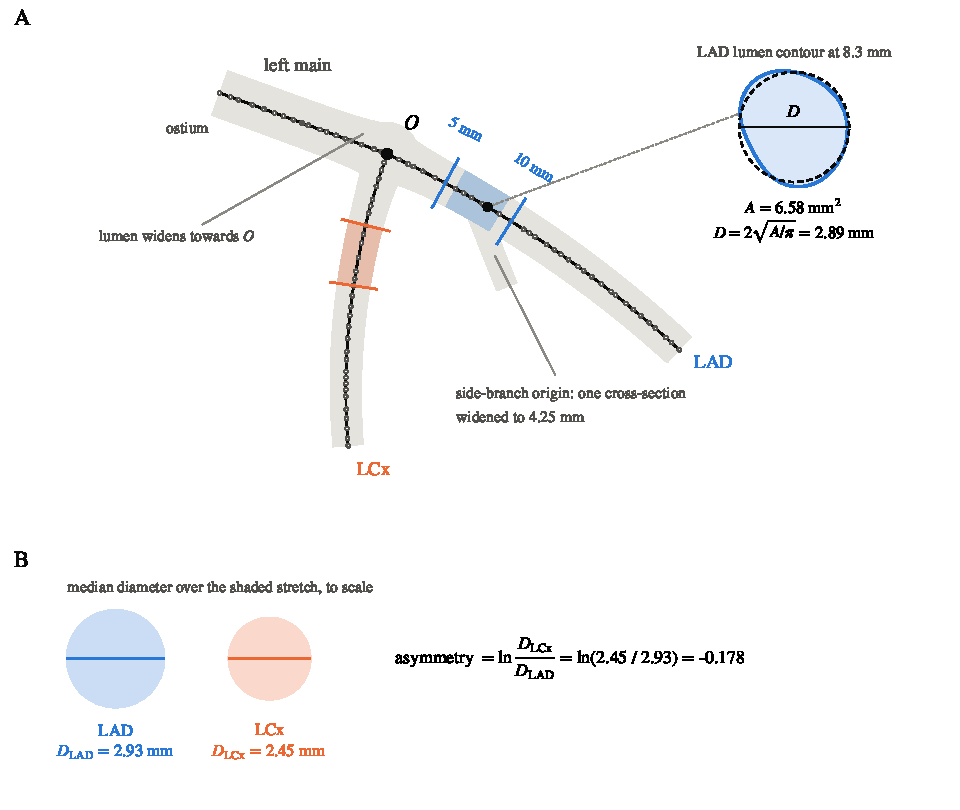
\includegraphics[width=\textwidth]{content/methodology/figures/daughter_ratio_figure.pdf}
  \caption{Daughter asymmetry on a made-up left main bifurcation, computed with the thesis code. Each lumen contour is reduced to the diameter $D$ of the circle with the same area, and the LAD and the LCx each to the median of $D$ over the shaded stretch 5 to 10\,mm from the bifurcation point $O$, which leaves out the widened lumen near $O$ and is not moved by the one cross-section widened at a side-branch origin (A). The two diameters, drawn to scale, give the daughter asymmetry (B).}
  \label{fig:method-ratio}
\end{figure}

% NOTES ONLY, to be written. Trimmed 2026-11-07 from thesis/methodology/05d_taper.tex
% (full draft in git, commit e4eb857). Implementation: tortuosity/taper.py, not yet in
% CGPS_data/thesis_final/.
%
% The subsection should contain:
% - Rationale: steady-flow WSS = 4 mu Q / (pi r^3) (malek1999shear); flow falls along the artery
%   with side branches, and with the pooled exponent 2.39 (taylor2024murray) taper carries only part
%   of the signal. Evidence for taper is thin (sec:lit-wss), no study links it to later plaque.
%   Log-radius slope is independent of overall calibre. Expected sign: lower taper -> lower WSS ->
%   more plaque, but sub-detection wall thickening could give the opposite sign. Open: two-sided
%   or signed test.
% - Size of the effect: about 0.25 mm diameter per 10 mm in normal arteries (medranogracia2016atlas),
%   about one voxel over 30 mm, so a robust fit over many cross-sections.
% - Computation in taper.py: resample every 0.5 mm; tangent from points 2.5 mm before and after;
%   orthogonal cut on a 12 x 12 mm grid at 0.1 mm, trilinear mask, threshold 0.5; area of the
%   connected region containing the centerline point; area-equivalent radius r = sqrt(A/pi)
%   (distance-transform radius kept for sensitivity). Open: how a voxel mask is formed from the
%   tracer's lumen contours.
% - Exclusions: first 3 mm, within two median radii of a side-branch junction, centerline point
%   outside the lumen, region touching the grid edge or another labelled vessel.
% - T = -10 b, b the Theil-Sen slope of ln r against s: fractional loss of radius per 10 mm.
%   Missing when remaining samples span < 20 mm or are < 60% of all samples.
% - Open: taper.py gives one T per artery, sec:method-selection uses taper per segment.
\subsection{Lumen Taper}
\label{sec:method-taper}

\todonote{To be written: rationale for taper and its Theil--Sen estimate from the lumen cross-sections.}


% NOTES ONLY, to be written. Trimmed 2026-11-07 from thesis/methodology/06_feature_validity.tex
% (full draft in git, commit e4eb857). Figure feature_validity_schematic.{py,pdf} still in
% thesis/methodology/. Detail for reproduction: appendix sec:app-validity. Results:
% results/01_feature_validity. Code: CGPS_data/hypertension_tortuosity.py; feature code in CGPS_data/thesis_final/
% (curvature_feature.py, bifurcation_angle.py, daughter_ratio.py, taper_feature.py; each has a --check on
% synthetic shapes that this section's accuracy study can build on). tortuosity/taper.py is the old voxel-mask code.
% Medis is deliberately not part of this section (it is in medis_reference, sec:method-medis).
% COSMIN taxonomy (mokkink2010cosmin), QIBA terminology (kessler2015qib, raunig2015qib).
%
% The section should contain:
% - Opening: without a reference standard, a null result cannot be told from a failed measurement,
%   so the features are checked indirectly and without the outcome. Repeatability not assessable
%   (no short-interval rescans; sec:disc-validity-repeatability). Primary definitions fixed before
%   any hypothesis is tested. Figure fig:method-validity: modest group difference, large spread.
% - Technical accuracy on synthetic shapes (sec:method-validity-accuracy): arcs, helices, sines,
%   tapering tubes, Y-tubes; smooth centerline displacement [..] to [..] mm and radius perturbation
%   incl. a bias growing as the vessel narrows; bias and linearity; error SD scaled by the
%   between-participant spread. Tests the computation, not the tracer. Phantom benchmark not written.
% - Definitional choices (sec:method-validity-definitions, with sec:method-validity-sensitivity):
%   table tab:method-validity-definitions of primary and alternative definitions per feature; chosen
%   on accuracy and literature, never on the hypotheses; every hypothesis recomputed per alternative.
%   Open: diameter windows (LAD/LCx 5 to 10 mm, LM first 2 mm), the angle's fitted stretch (5 to 10 mm,
%   chosen over lines from O, see appendix app:angle-origin), the taper exclusion radii and minimum length.
% - Construct validity (sec:method-validity-groups, sec:method-validity-evidence): prespecified
%   known-groups, internal-relationship and discriminant hypotheses with a size and direction
%   (table tab:method-validity, using only BL/FU header variables). Confirmed when the estimate is in
%   its range; no-difference hypotheses by a 90% CI within +-0.2 SD (lakens2017equivalence). Age
%   adjusted; body-size adjustment as in the source study. Evidence graded strong/moderate/weak.
%   Caveats: mostly referral cohorts, only a preprint measured curvature this way
%   (gharleghi2024leftmain), noise in narrow arteries can mimic the sex difference.
%   Open: confirm expected ranges before the data are opened.
% - Variance explained (sec:method-validity-split): R^2 of each feature on the base covariates;
%   1 - R^2 is room for geometry, but it cannot be split into anatomy and error without rescans.
% - Decision rules (sec:method-validity-reading): keep if all strong hypotheses confirmed; else check
%   extraction, then the alternative with the smallest scale-free error, never the best-fitting one.
%   Open: what happens if no alternative passes; the date everything was fixed.
\section{Measurement Properties of the Geometric Features}
\label{sec:method-validity}

\todonote{To be written: technical accuracy, definitional choices, construct validity, variance explained by known risk factors and the decision rules. See the notes in the source.}

\subsection{Technical Accuracy on Synthetic Shapes}
\label{sec:method-validity-accuracy}

\subsection{Definitional Choices}
\label{sec:method-validity-definitions}
\label{sec:method-validity-sensitivity}

\subsection{Construct Validity}
\label{sec:method-validity-groups}
\label{sec:method-validity-evidence}

\subsection{Variance Explained by Known Risk Factors}
\label{sec:method-validity-split}

\subsection{Decision Rules}
\label{sec:method-validity-reading}

% NOTES ONLY, to be written. Trimmed 2026-11-07 from thesis/methodology/07_curvature_fpca.tex
% (full draft in git, commit e4eb857). Decision 2026-11-04: main model uses mean curvature; FPCA
% shape scores only in pLAD and mLAD, each its own descriptive cloglog model, not pooled, not part
% of the LR test. Theory: sec:tech-fpca, sec:tech-fpca-grid, sec:tech-fpca-registration.
% Settings: CGPS_data/turning_profile_shapes.py and segment_k_budget.py, neither in thesis_final;
% turning_profile_shapes still runs on the Medis trees.
%
% The section should contain:
% - Why: mean curvature gives the same value to one sharp bend and to even turning; FPCA of the
%   profile describes where along the segment the turning lies. Secondary, descriptive, outside the
%   test of the geometry block (sec:method-models). Restricted to pLAD and mLAD for events ([..]).
% - Profile (eq:method-profile) on 50 equally spaced points of normalised position, linear
%   interpolation; FPCA per segment by SVD of the centred participant x grid matrix; no registration,
%   so a component can also be a shift of a bend.
% - K fixed before outcome linkage: smaller of [rule] and the Riley budget of the segment less the
%   base. Open: which rule (80/90% variance, Horn, circular-shift null, bootstrap |cos| >= 0.9,
%   5-fold CV error).
% - Per segment a cloglog model with the base and K scores, one row per participant, estimates with
%   intervals, not tested. Open: the base (1 df, recalibrated SCORE2, in segment_k_budget.py) and
%   the interval method.
\section{Secondary Analysis of Curvature Shape}
\label{sec:method-fpca}

\todonote{To be written: FPCA of the curvature profile in the proximal and mid LAD as a descriptive secondary analysis.}


\chapter{Experiments and Results}
\label{ch:results}

\section{Baseline segmentation}
\label{sec:baseline}

The figure and table you showed your supervisor in week 7 go here, unchanged.


\chapter{Discussion}
\label{ch:discussion}

\section{Limitations}
% NOTES, to be written (moved 2026-11-09 from Technical sec:tech-fpca, where they were general
% statements; here they become limitations of the descriptive FPCA, Methods sec:method-fpca):
% - Components are built from the curves alone and ranked by variance (wang2016fda, p. 26), and K
%   keeps only the leading, bootstrap-stable components within the Riley budget. A low-variance
%   shape that relates to plaque could therefore be left out, so a null association of the scores
%   does not show that profile shape is irrelevant.
% - The components rest on the covariance, a second moment, so a few outlying curves can shift
%   them (wang2016fda, p. 11). In the turning profiles, tracer errors (kinks, mis-tracked
%   stretches) give such curves. The bootstrap stability rule guards in part: a component driven
%   by a few curves changes between bootstrap samples and fails the check. State whether outlying
%   profiles were inspected or excluded once the FPCA code is in thesis_final/.
% - The components are specific to the sample and the preprocessing they were estimated from
%   (moved 2026-11-09 from sec:tech-fpca; uncited reasoning). Components from the Medis trees
%   (plaque at baseline) need not carry over to the plaque-free tracer cohort, and changing the
%   5 mm chord, the segment division or the grid would change the shapes. Components from another
%   cohort or study are therefore not directly comparable.
% - Position error in the tortuosity feature (moved 2026-11-09 from Methods sec:method-curvature,
%   05a_curvature.tex). Methods keeps only the reason for the 5 mm chord and its cost. Here: the
%   errors in the tracer point positions are likely of the order of the voxel size
%   \clarify{voxel size of the CGPS scans and the position precision of the tracer points}. In the
%   sliding window an error at the centre point tilts both of its chords at once, and since every
%   angle counts as positive, the false turns add up instead of cancelling, so they raise T most on
%   nearly straight segments and may differ between scans with different image noise. This is
%   measurement error in a predictor, which tends to pull its hazard ratio towards 1 (CITATION
%   WANTED for regression dilution); a null result for tortuosity is therefore weaker evidence of no
%   association. Give the size once Kit answers; no ImageCAS-X numbers.
% - Scale of the curvature values (2026-11-10, from the two papers read in full). Absolute curvature
%   depends on the scale at which it is estimated: van Zandwijk et al. (vanzandwijk2019curvature,
%   Menger's formula at 5 mm, as here) report 0.078 to 0.090 mm^-1, while Kashyap et al.
%   (kashyap2022tortuosity, VMTK-smoothed centerlines resampled at 0.01 mm, first 10 mm after the LM
%   bifurcation) report 0.40 to 0.51 mm^-1. CGPS values therefore compare only with studies at the
%   same scale; hazard ratios per SD are unaffected by the scale only if the ordering of segments
%   is. Uncited reasoning apart from the two values.
% - Cardiac phase (same source): van Zandwijk et al. found curvature 9% to 11% higher at end-systole
%   than at end-diastole, so the reconstruction phase is a source of variation in the feature.
%   CHECK: CGPS reconstruction phase (sec:data-cohort, blank) and whether it varies between scans.
% - Bends in the bifurcation angle (moved 2026-11-11 from Methods sec:method-angle, 05b). The
%   direction of each artery is a line fitted over 5 to 10 mm from O, so a bend within that stretch
%   also enters theta: on two arteries leaving 60 deg apart and curving away on 30 mm circles, the
%   fitted angle is 88.6 deg (bifurcation_angle.py --check; appendix app:angle-origin). The angle
%   therefore mixes the opening of the bifurcation with the early curvature of the arteries. Cardiac
%   phase also matters: the left main angle varies by about 11 deg between systole and diastole
%   (Girasis et al. 2010, SYNTAX substudy, 3D QCA; CITATION WANTED, not in refs.bib, full text not read).
\section{Future work}

\chapter{Conclusion}
\label{ch:conclusion}


\printbibliography[heading=bibintoc]

\appendix

% Appendix to sec:method-angle (05b_bifurcation_angle.tex): why the angle is measured 5 to 10 mm from O
% with a fitted line. Written 2026-11-11 from the explanation given to the user in session.
% The O-placement argument is the thesis's own; Medrano-Gracia et al. give only "average in the 5-10 mm
%   depth interval where variation is typically small" and "averaging angles in the 5-10 mm interval
%   ensures a more robust measurement than a single point" (PDF read 2026-11-11).
% Numbers: Table app-angle-tilt from a scratchpad numpy script (two straight arteries 75 deg apart, O 1 mm
%   upstream along the left main axis, points at 2, 5, 10 mm from the true split): 50.4, 63.0, 68.5 deg.
%   Table app-angle-offset and the bend case from CGPS_data/thesis_final/bifurcation_angle.py --check.
% CHECK: "a millimetre or more" is reasoning, not a measured tracer error; compare O on the tracer trees
%   with the Medis bifurcation once both are available.
\chapter{Placement of the Bifurcation Point}
\label{app:angle-origin}

The bifurcation angle of Section~\ref{sec:method-angle} is measured from the bifurcation point $O$, the last centerline point shared by the LAD and the LCx.
This point can only be placed approximately.
Where the two lumens merge, the centerline runs through the middle of the widened confluence, so the point at which the paths of the two arteries separate depends on the segmentation and on how the tracer joins them rather than on a sharp anatomical landmark.
An error in $O$ of a millimetre or more is therefore plausible.

Such an error matters most for directions measured close to $O$.
If the direction of an artery is taken as the line from $O$ to a point on it, a misplaced $O$ tilts that line, and the tilt shrinks as the point moves further away.
Table~\ref{tab:app-angle-tilt} shows this for two straight arteries 75 degrees apart with $O$ placed 1\,mm upstream of the true split: measured to points 2\,mm along the arteries, the angle reads 50.4 degrees, and measured to points 10\,mm along, 68.5 degrees.

\begin{table}[htbp]
  \centering
  \caption{Angle between the lines from a bifurcation point placed 1\,mm upstream of the true split to points on two straight arteries 75 degrees apart, by the distance of the points from the true split.}
  \label{tab:app-angle-tilt}
  \begin{tabular}{lccc}
    \hline
    Distance from the true split (mm) & 2 & 5 & 10 \\
    Measured angle (degrees) & 50.4 & 63.0 & 68.5 \\
    \hline
  \end{tabular}
\end{table}

Two choices keep the angle of this thesis from depending on $O$.
The arteries are represented only from 5\,mm onwards, and the direction of each is a straight line fitted through its points between 5 and 10\,mm, which does not pass through $O$.
Moving $O$ then only shifts the fitted stretch slightly along the artery.
On the same two straight arteries, the fitted angle stays at 75 degrees for every position of $O$ up to 3\,mm upstream, whereas the angle between the lines from $O$, averaged over the same depths, falls to 43.7 degrees (Table~\ref{tab:app-angle-offset}).

\begin{table}[htbp]
  \centering
  \caption{Bifurcation angle of two straight arteries 75 degrees apart when the bifurcation point $O$ is placed upstream of the true split, measured with the fitted lines of Section~\ref{sec:method-angle} and with lines from $O$ averaged over depths 5 to 10\,mm.}
  \label{tab:app-angle-offset}
  \begin{tabular}{lccccc}
    \hline
    $O$ upstream of the true split (mm) & 0 & 0.5 & 1 & 2 & 3 \\
    Fitted lines (degrees) & 75.0 & 75.0 & 75.0 & 75.0 & 75.0 \\
    Lines from $O$ (degrees) & 75.0 & 70.1 & 65.0 & 54.5 & 43.7 \\
    \hline
  \end{tabular}
\end{table}

The cost of the fitted line is that a bend within the 5 to 10\,mm stretch enters the angle.
For two arteries that leave the bifurcation 60 degrees apart and curve away from each other on circles of 30\,mm radius, the fitted angle is 88.6 degrees and the averaged angle from $O$ 74.3 degrees.
The interval itself follows Medrano-Gracia et al., who chose it because the angle varies little with depth there \cite{medranogracia2016atlas}.

\chapter*{Use of generative AI}
\addcontentsline{toc}{chapter}{Use of generative AI}

Large language models were used in this project for code troubleshooting,
figure generation and language refinement of the written report, in accordance
with DTU's guidelines for documenting the use of generative AI. All output was
reviewed and verified by the author. The methodology, analysis and conclusions
are the author's own.


\end{document}
